\documentclass[a4paper]{tufte-book}

\def\withcolors{1}
\def\withnotes{1}
\usepackage{ccanonne}
\usepackage{additionalnotation}

\usepackage{fontawesome5}
\newcommand{\ball}[1][red]{\text{\textcolor{#1}{\footnotesize\faBaseballBall}}\xspace}
\newcommand{\balla}[1][red]{\text{\textcolor{#1}{\footnotesize\faBaseballBall}}\xspace}
\newcommand{\ballb}[1][blue]{\text{\textcolor{#1}{\footnotesize\faBasketballBall}}\xspace}
\newcommand{\bin}[1][brown]{\text{\textcolor{#1}{\faBoxOpen}}}
\newcommand{\red}[1]{\textcolor{red}{#1}}
\newcommand{\blue}[1]{\textcolor{blue}{#1}}
\newcommand{\orange}[1]{\textcolor{orange}{#1}}
\newcommand{\green}[1]{\textcolor{ForestGreen}{#1}}
\newcommand{\purple}[1]{\textcolor{RoyalPurple}{#1}}

\newcommand{\advancedstuff}{($\star\star$)\xspace}

\title{COMP\textsubscript{4}\textsuperscript{5}270: Randomised and Advanced Algorithms}
\author{Cl\'ement Canonne}
\date{2024}


\renewcommand{\maketitlepage}{%
  \cleardoublepage
  {%
  \sffamily
  \begin{fullwidth}%
  \fontsize{18}{20}\selectfont\par\noindent\textcolor{darkgray}{\allcaps\thanklessauthor}%
  \vspace{11.5pc}%
  \fontsize{34}{40}\selectfont\par\noindent\textcolor{darkgray}{\allcaps\thanklesstitle}%
  \vfill
  \fontsize{14}{16}\selectfont\par\noindent\thanklesspublisher%
  \end{fullwidth}%
  }%
  \thispagestyle{empty}%
  \clearpage
}

\begin{document}
\frontmatter
\maketitle
This course will provide a rigorous introduction to a range of techniques and paradigms central to modern algorithm design, with a focus on randomised algorithms. The course will 
emphasise the theoretical underpinnings of these algorithms and their mathematical guarantees, and provide intuition and understanding through a range of practical applications and examples such as probabilistic data structures, hashing, approximation algorithms, and streaming algorithms.


\paragraph{Outline of the course (some topics are tentative):}
\begin{enumerate}
    \item Discrete Probability for Algorithm Designers: expectation, variance, independence. Randomised algorithms (definitions, motivating examples). Linearity of expectation and applications.
    \item Concentration bounds, probability amplification. Median trick.
    \item Coupon Collector, Load Balancing, Power of Two Choices
    \item Derandomisation: Max-Cut, Method of Conditional Expectations
    \item Graph algorithms: Randomized Min-Cut (Karger’s algorithm), MST in expected linear time (Karger, Klein, and Tarjan), possibly Bipartite Matching (Mulmuley, Vazirani, and Vazirani)
    \item Probabilistic data structures I: Hashing and Bloom filters
    \item Probabilistic data structures II: Johnson-Lindenstrauss, LSH
    \item Streaming and Sketching I: definitions, examples, frequency estimation
    \item Streaming and Sketching II: CountSketch, Count–min Sketch
    \item Linear Programming and Randomised Rounding
    \item Randomised Embeddings: FRT algorithm, and applications
    \item Sampling and Counting
    \item Review
\end{enumerate}

\tableofcontents

\listoffigures

\listoftables
\mainmatter

\chapter*{Before we start}
Things you are assumed to know.
\begin{enumerate}
    \item Big-Oh notation and worst-case analysis. In this class, and in algorithm design and theory of algorithms and computer science in general,
we extensively use two things: worst-case analysis and big-Oh notation. Those two things often come together, but they are not the same thing: they just
complement each other. You're expected to be familiar and comfortable with both of them, and to know the difference.
    \item Writing proofs, rigorously and preferably concisely.
    \item \TODO
\end{enumerate}

\chapter{Lecture 1: Randomness, Probability, and Algorithms}

%%%%%%%%%%%%%%%%%%%%%%%%%%%%%%%%%%%%%%%%%%%%%%%%%%%%%%%%%%%%%%%%%%%%%%%%%%
Take a standard deck of 52 cards, with 13 $\spadesuit$, 13 $\heartsuit$, 13 $\diamondsuit$, and 13~$\clubsuit$. Shuffle it (well), so that the order is completely (uniformly)\footnote{People usually say ``random'' when they mean \emph{uniformly} random, and that can be quite ambiguous. I'll try not to.} random. \emph{How many consecutive pairs of the same suit do you expect?}

\begin{comment}
deck = StringJoin@*Reverse /@ 
  Tuples[{{"$\[SpadeSuit]$", "$\[HeartSuit]$", "$\[DiamondSuit]$", 
     "$\ClubSuit$"}, 
    Join[{"A"}, ToString /@ Range[2, 10], {"J", "Q", "K"}]}]
ResourceFunction["Shuffle"]["RandomSample"][deck]
\end{comment}

For instance,
\begin{center}
4$\heartsuit$, 3$\heartsuit$, 8$\clubsuit$, 2$\clubsuit$, 3$\spadesuit$, 10$\heartsuit$, 8$\diamondsuit$, 7$\spadesuit$, K$\heartsuit$, 5$\diamondsuit$, 8$\heartsuit$, J$\heartsuit$, 9$\clubsuit$, \\
5$\clubsuit$, J$\spadesuit$, 2$\heartsuit$, Q$\spadesuit$, 2$\spadesuit$, 10$\spadesuit$, 6$\spadesuit$, 6$\clubsuit$, 5$\heartsuit$, 4$\clubsuit$,  9$\spadesuit$,  Q$\diamondsuit$,  8$\spadesuit$,  \\
6$\diamondsuit$, 10$\diamondsuit$, 7$\clubsuit$, J$\clubsuit$, K$\clubsuit$, 4$\diamondsuit$, K$\diamondsuit$, K$\spadesuit$, A$\diamondsuit$, A$\spadesuit$, A$\clubsuit$, 4$\spadesuit$, A$\heartsuit$,  \\
3$\clubsuit$, 9$\diamondsuit$, 3$\diamondsuit$, J$\diamondsuit$, 9$\heartsuit$, Q$\heartsuit$, Q$\clubsuit$, 2$\diamondsuit$, 10$\clubsuit$, 5$\spadesuit$, 7$\diamondsuit$, 6$\heartsuit$, 7$\heartsuit$
\end{center}
has 15 such consecutive pairs.\marginnote{Please check.}

So\dots what's the expected number of consecutive same-suit pairs in a shuffled deck?

Let's try to estimate this:
\begin{lstlisting}
import numpy as np
import random
deck = 13*['S', 'H', 'D', 'C']
consecutives = []
for _ in range(50000):
    shuffled_deck = random.sample(deck, len(deck));
    consecutives += [np.sum([shuffled_deck[i] == shuffled_deck[i+1] for i in range(len(deck)-1)])]
print("Empirical mean: %f" % np.mean(consecutives))
\end{lstlisting}
I ran it: this gave $11.98176$. I ran it again: $12.0022$. And these 50,000 attempts look roughly like this (\cref{fig:consecutives}):
\begin{lstlisting}
import matplotlib.pyplot as plt
plt.hist(consecutives, density = True, bins=25, edgecolor='k');
plt.axvline(np.mean(consecutives), color='r', linestyle='dashed', linewidth=2)
plt.show()
\end{lstlisting}
\begin{figure}[htbp]\centering
    \label{fig:consecutives}
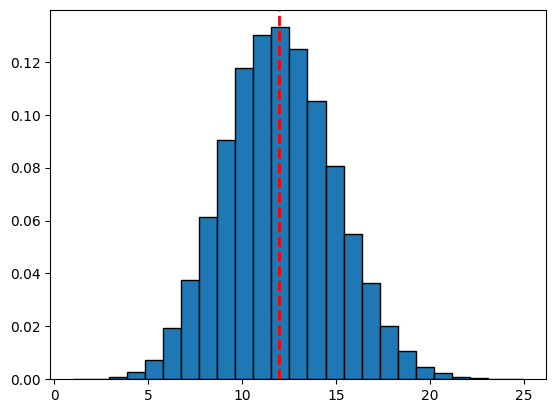
\includegraphics[width=0.7\textwidth]{figures/fig-consecutives-shuffled.png}
\caption{(Normalized) histogram of the number of consecutive pairs of the same suit, over $50,000$ trials. The red dashed line is the empirical mean.}
\end{figure}
Looks like this expected number is something like 12.\marginnote{Try to see what changes if you change the number of cards in the deck (for instance, 34 cards from each suit instead of 13). Could you have predicted it?} How do we explain this?

\begin{theorem}
    The expected number of consecutive same-suit pairs is 12.
\end{theorem}
\begin{proof}
    ``Linearity of expectation.''\marginnote{$\forall i$, $\probaOf{X_i = X_{i+1}} = \frac{13-1}{52-1}$}
\end{proof}

\subsection{One for the rainy days.} It's raining, and all $n$ students of the class come to the lecture with an umbrella. They all leave it in front of the lecture hall. At the end of the lecture, they leave the room in (uniformly) random order, and crossing the door each takes the closest remaining umbrella. In expectation, \emph{how many leave with their own umbrella}?

\begin{theorem}
    The expected number of fixed points in a uniformly random permutation of $\{1,2\dots,n\}$ is one.
\end{theorem}

%%%%%%%%%%%%%%%%%%%%%%%%%%%%%%%%%%%%%%%%%%%%%%%%%%%%%%%%%%%%%%%%%%%%%%%%%%
\section{What's a randomized algorithm?}
Randomized algorithms are algorithms whose behaviour \emph{does not
depend solely on the input.} It also depends (in part) on random
choices or the values of a number of \emph{random bits}.\smallskip

So we can think of the algorithm $\Algo$ as taking an input $x$ and a string of uniformly random bits $R\in\bool^\ast$. Now, since $\Algo$ is randomised, this could mean several things:
\begin{enumerate}
    \item The time $\tau_{\Algo}(x; R)$ that $\Algo$ takes on input $x$ is itself random, and depends on the random bits $R$
    \item The output $\Algo(x;R)$ of $\Algo$ on input $x$ is random, and can be different based on the random bits $R$
    \item Something else (\eg the amount of memory used by $\Algo$ could depend on the random bits)
    \item all, or any combination of the above
\end{enumerate}

Typically, what we want is then analyze $\Algo$ on \emph{worst-case} input $x$ and \emph{uniformly random} $R$. The two things to keep in mind: (1)~is the output of $\Algo$ always correct? Is it correct with high probability (over the choice of random bits $R$)? (2)~is the running time of $\Algo$ always bounded? Is it bounded with high probability, or in expectation (over the choice of random bits $R$)?\marginnote{\advancedstuff{} For those interested, for decision problems this is related to complexity classes \textsf{ZPP}, \textsf{RP}, and \textsf{BPP}. Think of that last one as ``randomized \textsf{P}.''}

\begin{description}
    \item[Las Vegas algorithms:] the algorithm is \emph{always correct}, but the running time is only bounded \emph{in expectation}. 
    \item[Monte-Carlo algorithms:] the algorithm is only \emph{correct with high probability}, but the running time is bounded \emph{with probability one}. 
\end{description}

This is very abstract right now, so before moving to the subtantial example of QuickSort (soon), here is an example:
\begin{framed}
    Given an (arbitrary) array of size $\ns$ containing all numbers from $1$ to $\ns$, output the index of an even number.
\end{framed}
\begin{claim}[Bad news]
Any deterministic algorithm  for this task must have worst-case time complexity $\Omega(\ns)$.
\end{claim}
\begin{claim}[Good news]
There is a Las Vegas algorithm for this task with \emph{expected} time complexity $O(1)$.
\end{claim}
% Pick one until you find one. Expected timesum_k k/2^k = O(1)
\begin{claim}[Good news]
There is a Monte Carlo algorithm for this task with \emph{worst-case} time complexity $O(1)$, and probability of success $0.99$.
\end{claim}
% Pick one k=log2(100) times: failure <= 1/100

\subsection{Relation to other notions of analysis.} What you have focused so far in algorithms classes is \emph{worst-case analysis}: this quantifies the worst possible behaviour of an algorithm (its time complexity, or space complexity, usually), that is, how badly it will do \emph{on the worst possible input you can give it}. This is very useful to know, since once you have figured that out then you know that, no matter what, your
algorithm cannot do worse than that, even on the most adversarial situation. But there are other types of analysis, less frequent and usually much harder to interpret, that can be used: \emph{expected
time analysis} (when the algorithm is randomized: \textbf{this class}), \emph{average time analysis} (when
the input itself comes from some known probability distribution: \textbf{not now}), \emph{amortized
analysis} (when we use the algorithm repeatedly on a sequence of inputs, and look at the worst-case sequence of input for the algorithm divided by the length of the sequence).

\paragraph{Summary:} if $\tau_{\Algo}(x)$ is the time taken by $\Algo$ on input $x$ of size
$|x|$ and $\Algo_k(x_1,\dots,x_k)$ corresponds to running the algorithm successively on
inputs $x_1, \dots, x_k$, then the time analyses discussed above correspond to:
\begin{align*}
    T(\ns) &= \max_{x: |x|=\ns} \tau_{\Algo}(x) \tag{Worst-case} \\
    T_{\rm{}expected}(\ns) &= \max_{x: |x|=\ns} \bE{R}{\tau_{\Algo}(x;R)} \tag{Expected: $\Algo$ is randomized} \\
    T_{\rm{}average}(\ns) &= \bE{x}{\tau_{\Algo}(x)} \tag{Average-case: $x$ is random} \\
    T_{\rm{}amortized}(\ns) &= \lim_{k\to\infty} \frac{1}{k}\max_{|x_1|=\dots=|x_k|=\ns} \tau_{\Algo_k}(x_1,\dots,x_k) \tag{Amortized}
\end{align*}
Again, you probably focused on the first in previous studies, and in this unit we will also consider the second.

\subsection{But why?}
\noindent Some of the reasons for using randomization:
\begin{itemize}
    \item Quickly finding representative or relevant parts of the input (\eg sampling data from a large dataset)
    \item Avoid pathological corner cases
    \item Avoid predictable outcomes % Cryptography, privacy
    \item Allow for simpler or more efficient algorithms
    \item \dots\marginnote{Can you think of anything else?}
\end{itemize}
Some drawbacks:
\begin{itemize}
    \item The behaviour of the algorithm is, well, random. The output might be, or the running time, or something else. Are you happy with this non-deterministic behaviour?
    \item Where do you find these ``random bits'' the algorithm needs?\marginnote{Any idea?}
\end{itemize}
%%%%%%%%%%%%%%%%%%%%%%%%%%%%%%%%%%%%%%%%%%%%%%%%%%%%%%%%%%%%%%%%%%%%%%%%%%
\section{Analyzing Randomized Quicksort}\marginnote{Is this a Las Vegas or a Monte Carlo algorithm?}

Remember QuickSort from your previous classes? It's a very nice comparison-based sorting algorithm, which works as follows:
\begin{algorithm}
\begin{algorithmic}[1]
    \Require Input array $A$ of size $\ns$
    \If{$\ns\leq 1$} \Return $A$
    \EndIf
    \State\label{algo:line:pivot} Select an index $1\leq i\leq \ns$, and let $p \gets A[i]$ be the \emph{pivot}
    \State Partition $A$ into 3 subarrays: $A_1$ (elements smaller than $p$), $A_2$ (equal to $p$), and $A_3$ (greater than $p$) \Comment{ $O(\ns)$ time}
    \State Recursively call QuickSort on $A_1$ and $A_3$ to sort them
    \State Merge the (sorted) $A_1$, $A_2$, $A_3$ into $A$ \Comment{ $O(\ns)$ time}
    \State \Return $A$
\end{algorithmic}
\caption{\textsc{QuickSort}}
\end{algorithm}
This is the prototypical example of a divide-and-conquer algorithm: the only thing unspecified above is \emph{how to choose the pivot}. And this is very important: the time complexity of the whole algorithm depends crucially on it!

The naive way to choose the pivot deterministically (just pick, say, $i=\clg{\ns/2}$) is quite terrible, leading to a worst-case time complexity of $O(\ns^2)$. Not so ``quick.'' A much more involved way to do so, getting the \emph{median} as pivot using linear-time selection\marginnote{If you don't remember what it is, that's alright~--~but it's worth looking it up.} does give sorting in worst-case $O(\ns\log\ns)$ time: but now the algorithm is very complicated, and not so fast in practice anymore.

But this is a class on randomized algorithm, so let's do the obvious randomized thing, and pick the pivot uniformly at random: in~\cref{algo:line:pivot}, choose $i$ uniformly at random in $\{1,2,\dots,\ns\}$. This gives us \emph{Randomized QuickSort}. The proof of correctness is the same as usual QuickSort, but what about the (expected) time complexity? \emph{How fast is it?}

Well, the expected time complexity $T(\ns)$ satisfies the recurrence:
\begin{equation}
    \label{eq:quicksort}
T(\ns) = \bEE{T(|A_1|) + T(|A_2|)} + O(\ns)
\end{equation}
where the expectation is over the random choice of pivot in~\cref{algo:line:pivot}; and $T(1) = O(1)$.

Suppose for simplicity that all elements are distinct.\marginnote{Curious? See how to adapt the proof below to the general case.} Then, if pick pick as pivot the $k$-th largest element, $n_L=k-1$ and $n_R = n-k$. What is the probability to pick the $k$-th largest element as pivot? We select the pivot uniformly at random, so that's $1/n$.

So we can rewrite (the $c\ns$ is for the $O(\ns)$ in~\eqref{eq:quicksort}, which comes from the Divide and the Conquer steps): 
\begin{align*}
 T(\ns) &= c \ns + \frac{1}{n}\sum_{k=1}^{\ns} (T(k-1)+T(\ns-k) ) \\
&= c \ns + \frac{1}{\ns}\sum_{k=0}^{\ns-1} {T(k)}+ \frac{1}{\ns}\sum_{\ell=0}^{n-1} {T(\ell)}
\end{align*}
That is,
\begin{align}
\label{eq:quicksort:rand}
T(\ns) = c \ns + \frac{2}{\ns}\sum_{k=0}^{\ns-1} {T(k)}
\end{align}
Now, \emph{how do we solve this?}\marginnote{Any idea?}

\paragraph{First method: guess, and prove inductively.}
You know the drill. Magically guess $T(\ns) \leq a\ns\log\ns$, try to prove it by induction, see it doesn't quite work depending on which bound you use for $\sum_{k=1}^\ns k\log k$, maybe change your ``magic guess'' to $T(\ns) \leq a\ns\log\ns - b\ns$ to make it work (or get a better bound for the sum).

\paragraph{Second method: integrals are nicer than sums.}
Instead of solving~\cref{eq:quicksort:rand} directly, let's instead compare this discrete relation to a (much nicer to solve) differential equation. The idea is that often, ``sums and integrals are basically the same thing,''
\begin{fact}
    Let $f$ be a non-decreasing function. Then, for all $\ns \geq 0$,
    \[
        \int_0^\ns f(x)dx \leq \sum_{k=0}^\ns f(k) \leq \int_1^{\ns+1} f(x)dx
    \]
\end{fact}
Let's apply that here, and solve the functional equation\marginnote{We make a few implicit (reasonable) assumptions on $T$ here: which ones?}
\[
T(x) = cx + \frac{2}{x}\int_{0}^x T(u) du, \qquad x>0
\]
Introducing the antiderivative $F(x) = \int_{0}^x T(u) du$, we can rewrite this as 
\begin{align}
\label{eq:quicksort:diff:eq}
F'(x) = cx + \frac{2}{x}F(x)
\end{align}
which is ``easier'' to solve,\footnote{Check with an automated solver like Mathematica first: \url{https://www.wolframalpha.com/input?i=solve+F\%27\%28x\%29+\%3D+c+x+\%2B+2\%2Fx+F\%28x\%29+}.} and will lead to $T(x) = O(x \log x)$ and so $T(\ns) = O(\ns\log\ns)$. The point is that differential equations are often much easier to solve than discrete recurrence relations.

\paragraph{\advancedstuff How:} dividing everything by $x^2$, \cref{eq:quicksort:diff:eq} becomes $$ \frac{F'(x)}{x^2} - \frac{2}{x^3} F(x) = \frac{c}{x} $$ but then, we can use that $\frac{d}{dx} \frac{F(x)}{x^2} = \frac{F'(x)}{x^2} - \frac{2F(x)}{x^3}$, so integrating we get $$ \frac{F(x)}{x^2} = c\ln x + C $$ for some constant $C\in\mathbb{R}$, and so $F(x) = c x^2 \ln x + C x^2$. Then $f(x)=F'(x) = 2c x \ln x + (2C+1) x = O(x \log x)$, and we are done.

What we have shown is the following:
\begin{theorem}
    Randomized QuickSort has expected running time $\bigO{\ns\log\ns}$.\marginnote{But still worst-case running time $O(\ns^2)$.}
\end{theorem}

What about the number of \emph{comparisons}? Clearly, what we just showed implies that the expected number of comparisons is also $\bigO{\ns\log\ns}$, but if that's all we are interested in, could we have proven it in a nicer way?
\begin{theorem}
    The expected number of comparisons performed by Randomized QuickSort is $\bigO{\ns\log\ns}$.
\end{theorem}
\begin{proof}
    When we run QuickSort, all the comparisons at one level of the recurrence are between the current pivot and all the other $\ns-1$ elements, and we never compare two elements twice. So we \emph{could} try to solve the corresponding recurrence on the expected number of comparisons $C(\ns)$:
    \begin{equation}
    \label{eq:quicksort:comparisons}
    C(\ns) = \bEE{C(|A_1|) + C(|A_2|)} + (\ns-1)
    \end{equation}
    We could, but we will not.\marginnote{This is the same as for $T(\ns)$, but with an explicit constant instead of $c$.} Instead, here's a slightly nicer argument based on linearity of expectation.

    Suppose for simplicity that all $\ns$ elements are distinct\marginnote{Intuitively, duplicate elements can only make the expected number of comparisons smaller. Can you argue why?} and let us denote them, in ranked order, by
    \[
    a_1 < a_2 < a_3 < \dots < a_\ns
    \]
    (note that this is only for the analysis, and that $a_i$ is not necessarily the element at index $i$ of $A$: the array is generally not already sorted!)
    For any two indices $i < j$, let $X_{ij}\in\{0,1\}$ be the indicator variable of whether Randomized QuickSort ever compares $a_i$ and $a_j$. Since the algorithm never compares twice the same two elements, we have that the total number of comparisons is 
    \[
        X \eqdef \sum_{i=1}^{\ns-1} \sum_{j=i+1}^\ns X_{ij}
    \]
    and $C(\ns) = \bEE{X}$. By linearity of expectation,
    \[
        C(\ns) = \sum_{i=1}^{\ns-1} \sum_{j=i+1}^\ns \bEE{X_{ij}}
        = \sum_{i=1}^{\ns-1} \sum_{j=i+1}^\ns \probaOf{a_i\text{ and } a_j \text{ are compared}}
    \]
    So it boils down to understanding the probability Randomized QuickSort ever compares two fixed distinct elements of the array. Suppose we are at the ${\blue{\ell}}$-th recursive step of the algorithm, with $a_i,a_j$ both in the current subarray of size $\ns_{\blue{\ell}}$, and we pick a pivot $p$:
    \begin{itemize}
        \item If $a_i < p < a_j$, then we will recurse on two disjoint subarrays, one containing $a_i$ and the other $a_j$, so that they will never be compared (decision made!). This happens with probability $\frac{j-i-1}{\ns_{\blue{\ell}}}$.
        \item If $p$ is either $a_i$ or $a_j$, then they will be compared~--~since elements are only compared to the pivot (decision made!). This happens with probability $\frac{2}{\ns_{\blue{\ell}}}$.
        \item Otherwise, they are not compared at this stage, but they both end up in the same subarray the algorithm recurses on, so the comparison could happen later on. This ``no decision either way yet'' happens with probability $1-\frac{j-i+1}{\ns_{\blue{\ell}}}$.
    \end{itemize}
    From the above, we have
    \[
        \probaCond{\substack{a_i\text{ and } a_j\\\text{ are compared}\\\text{at stage }{\blue{\ell}}} }{\substack{\text{Decision made}\\\text{at stage }{\blue{\ell}}}}
        = \frac{\frac{2}{\ns_{\blue{\ell}}}}{\frac{j-i-1}{\ns_{\blue{\ell}}}+\frac{2}{\ns_{\blue{\ell}}}}
        = \frac{2}{j-i+1}
    \]
    Overall, we can write
    \begin{align*}
        \probaOf{\substack{a_i\text{ and } a_j\\\text{ are compared}}}
        &= \sum_{{\blue{\ell}}=0}^\infty \probaCond{\substack{a_i\text{ and } a_j\\\text{ are compared}\\\text{at stage }{\blue{\ell}}} }{\substack{\text{Decision made}\\\text{at stage }{\blue{\ell}}}}
        \probaOf{\substack{\text{Decision made}\\\text{at stage }{\blue{\ell}}}}\\
        &= \sum_{{\blue{\ell}}=0}^\infty \frac{2}{j-i+1}\cdot \probaOf{\substack{\text{Decision made}\\\text{at stage }{\blue{\ell}}}} \\
        &= \frac{2}{j-i+1}\,,
    \end{align*}
    the last line since probabilities sum to one. 
    We are almost there: remember that we are interested in $C(\ns)$, which we now are able to express as
    \[
    C(\ns) = \sum_{i=1}^{\ns-1} \sum_{j=i+1}^\ns \frac{2}{j-i+1}
    = 2\sum_{i=1}^{\ns-1} \sum_{k=1}^{\ns-i} \frac{1}{k+1}
    \]
    This may not look so nice, but letting $H_k = \sum_{i=1}^k \frac{1}{k} \leq \ln k + 1$ denote the $k$-th Harmonic number, we get
    \[
    C(\ns) = 2\sum_{i=1}^{\ns-1}( H_{\ns-i+1} - 1 )
    = 2\sum_{i=2}^{\ns} ( H_i - 1 )
    \leq 2\sum_{i=2}^{\ns} \ln i \leq 2\ns\ln \ns
    \]
    (we even get an explicit upper bound, not just $O(\ns\log\ns)$).
\end{proof}


%%%%%%%%%%%%%%%%%%%%%%%%%%%%%%%%%%%%%%%%%%%%%%%%%%%%%%%%%%%%%%%%%%%%%%%%%%
\section{A few useful probabilistic facts}
Let $X$ be a random variable (r.v.) taking real values: for instance, in $\R$ or $\N$. We assume $X$ has an expectation and a variance.\footnote{This is not necessarily always true! Some random variables do not even have a well-defined expectation. For instance, the random variable defined on $\Z$ by $\probaOf{X=k} = \frac{1}{C}\cdot \frac{1}{1+k^2}$ with $C = 1+\pi\coth \pi$ (so that the probabilities sum to 1) is well-defined, but does not have an expectation since $\sum_{k\in\Z}k\cdot \probaOf{X=k}$ is not defined (does not converge).} A few useful things:
\begin{fact}
If $X$ takes values in $\N = \{0,1,2,\dots,\}$,
\[
\bEE{X} = \sum_{n=0}^\infty n\probaOf{X=n} = \sum_{n=1}^\infty\probaOf{X \geq n}
\]
\end{fact}
To remember whether the sum in the last expression starts at $n=0$ or $n=1$: either reprove it (a bit time-consuming), or take $X$ to be the ``useless'' random variable equal to 0 with probability 1. Then $\bEE{X}=0$, but $\sum_{n=0}^\infty\probaOf{X \geq n} = \probaOf{X \geq 0} = 1$. So we shouldn't have the term $n=0$.

\begin{fact}
If $X$ has a finite variance,
\[
\var[X] = \bEE{(X-\bEE{X})^2} = \bEE{X^2}-\bEE{X}^2
\]
\end{fact}
As a direct consequence, $\var[X]\leq \bEE{X^2}$ (sometimes useful).

\begin{lemma}[Jensen's Inequality]
If $f\colon\R\to\R$ is convex (and $\bEE{f(X)}$ is well-defined)
\[
f(\bEE{X}) \leq \bEE{f(X)}\,.
\]
For $f$ concave, the inequality is reversed.
\end{lemma}
To remember the direction: check with $f(x)=x^2$ (convex). The variance is non-negative, so $0 \leq \var[X] = \bEE{X^2}-\bEE{X}^2$.

\begin{fact}[Linearity of Expectation]
For any $X,Y$ and $a, b \in \R$,
\[
\bEE{aX+bY} = a\bEE{X}+b\bEE{Y}
\]
(We do \emph{not} need $X,Y$ to be independent!)
\end{fact}
\noindent This extends to more random variables: for instance, $\bEE{\sum_{i=1}^n X_i} = \sum_{i=1}^n \bEE{X_i}$. (No independence needed!)

\begin{fact}[Variance]
For any $X$ and $a \in \R$,
\[
\var[aX] = a^2 \var[X]\,.
\]
Moreover, if $X,Y$ are \emph{independent}, 
\[
\var[aX+bY] = a^2 \var[X]+b^2 \var[Y]\,.
\]
\end{fact}
More generally, \textbf{if} $X_1,\dots, X_n$ are mutually independent (or, weaker condition, \emph{pairwise independent}: any two $X_i,X_j$ with $i\neq j$ are independent, but $X_1,\dots, X_n$ as a whole might not be mutually independent.), then
\begin{equation}
\var\mleft[\sum_{i=1}^n X_i\mright] = \sum_{i=1}^n \var[X_i].
\end{equation}
The proof is not too hard: basically, since $\var[X] = \bEE{(X-\bEE{X})^2}$, consider 
$\bEE{\Paren{\sum_{i=1}^n (X_i-\bEE{X_i})}^2}$ and expand the square, then use linearity of expectation:
\begin{align*}
\var\mleft[\sum_{i=1}^n X_i\mright] 
&= \bEE{\sum_{i=1}^n\sum_{j=1}^n (X_i-\bEE{X_i})(X_j-\bEE{X_j})} \\
&= \bEE{\sum_{i=1}^n(X_i-\bEE{X_i})^2} + \bEE{\sum_{i\neq j} (X_i-\bEE{X_i})(X_j-\bEE{X_j})}\\
&=\sum_{i=1}^n\bEE{(X_i-\bEE{X_i})^2} + \sum_{i\neq j} \bEE{(X_i-\bEE{X_i})(X_j-\bEE{X_j})}
\end{align*}
The first term is exactly $\sum_{i=1}^n\var[X_i]$; the second, by pairwise independence, is 0, since $\bEE{(X_i-\bEE{X_i})(X_j-\bEE{X_j})} = \bEE{(X_i-\bEE{X_i})}\bEE{(X_j-\bEE{X_j})} = 0\cdot 0$.\medskip


Now, a few very trivial-looking (but useful!) facts. Suppose $X$ takes values in $\{0,1\}$, with $\probaOf{X=1}=p$ (this is a Bernoulli random variable). Then
\begin{itemize}
    \item $X^2=X$ (of course!), so $\bEE{X^2}=\bEE{X}=\probaOf{X=1}=p$
    \item That implies $\var[X] = \bEE{X^2}-\bEE{X}^2 = p-p^2 = p(1-p)$, which is at most $1/4$.\marginnote{Check it! $x(1-x)\leq 1/4$ for $x\in[0,1]$, and the maximum is at $x=1/2$.}
    \item That implies that for a Binomial $X\sim\binomial{n}{p}$, which is just the sum of $n$ \emph{independent, and identically distributed} (\iid) Bernoullis with parameter $p$,
    \[
        \bEE{X} = np, \qquad \var[X] = np(1-p)\,.
    \]
\end{itemize}
Finally, an \emph{indicator} random variable (for some ``event'' $E$) is just a Bernoulli random variable which is equal to 1 if the event occurs, and 0 otherwise (so, Bernoulli with parameter $\proba(E)$). Usually denoted $\indicSet{E}$.

\chapter{Lecture 2: Concentration Bounds, and Tricks}\label{chap:2}
\section{Markov goes to Las Vegas}

Remember from last lecture that we saw two types of randomised algorithms: {Las Vegas} and {Monte Carlo}.\marginnote{There are more, of course: \eg Bellagio algorithms. And others! Mathematicians and computer scientists clearly love gambling~--~look up Jacob Bernoulli when you have a chance.}

\begin{quote}
\begin{description}
    \item[Las Vegas algorithms:] the algorithm is \emph{always correct}, but the running time is only bounded \emph{in expectation}. 
    \item[Monte-Carlo algorithms:] the algorithm is only \emph{correct with high probability}, but the running time is bounded \emph{with probability one}. 
\end{description}
\end{quote}
Wouldn't it be nice if there was a way to go from one to the other? Well, as it turns out, there is:
\begin{lemma}
    \label{lemma:lvtomc}
    Suppose there exists a Las Vegas algorithm $\Algo$ for some task, with expected running time $\blue{T}$. Then there exists a Monte Carlo algorithm $\Algo'$ for the same task with \emph{worst-case} running time $O(\blue{T})$ and probability of failure $1/100$.
\end{lemma}
\begin{proof}
The proof is quite simple, and relies on analyzing the following:
\begin{algorithm}[H]
\begin{algorithmic}[1]
    \Require input $x$
    \State Run $\Algo$ on $x$ for at most $100\blue{T}$ steps
    \If{$\Algo$ terminated within $100\blue{T}$ steps}
        \State\label{markov:line:goodoutput}\Return $\Algo$'s output \Comment{Always correct}
    \Else 
        \State\label{markov:line:mehoutput}\Return an arbitrary output \Comment{Very likely wrong}
    \EndIf
\end{algorithmic}
    \caption{Algorithm $\Algo'$.}
\end{algorithm}
It should be quite clear that the above algorithm always runs in time at most $100\blue{T} + O(1) = O(\blue{T})$; and also that whenever we reach~\cref{markov:line:goodoutput}, the output of $\Algo'$ must be correct (because $\Algo$, once it terminates, is always correct). 

When we reach~\cref{markov:line:mehoutput} because $\Algo$ ``timed out,'' however, we cannot really say anything: maybe what we output is correct, but it's most likely wrong. So we'll just assume it's an incorrect output, and all we need to do to prove the lemma is to prove that $\Algo$ ``times out'' with probability at most $1/100$.

Importantly, all we can use to do so is what we know about $\Algo$, which is very little: we only know its expected running time is at most $\blue{T}$, and that running times are non-negative. That's not a lot to build on, but that's just enough for \emph{Markov's inequality}:

\begin{theorem}[Markov's inequality]
Let $X$ be a non-negative\marginnote{The ``non-negative'' assumption is crucial. It is definitely not true without!} random variable with $\bEE{X} < \infty$. For any $t > 0$, we have
\[  
  \bPr{ X \geq t } \leq \frac{\bEE{X}}{t}
\]
\end{theorem}
\noindent Applying this with $X$ being the running time of $\Algo$ and $t=100$ proves the lemma.
\end{proof}
\marginnote{Lecture cue: prove Markov's.}
%%%
% Should I mention the algorithmic Jensen paper?
%%%
\section{Markov and beyond: Randomised Median}
% Useful/good: https://www.cs.dartmouth.edu/~deepc/LecNotes/Rand/lec6.pdf
As mentioned in the previous lecture, there exists a very neat, highly non-trivial (deterministic) divide-and-conquer algorithm to find the median of (an array of) $\ns$ numbers in linear time. You have seen it in previous  So we will not analyze it again: instead, we will give a simple (Monte Carlo) randomized algorithm, also linear-time. 

The idea of the algorithm is relatively simple, yet surprisingly powerful: given as input an array $\red{A}$ of $\ns$ integers\marginnote{For simplicity, we will throughout assume $\ns$ is odd, and that all numbers are distinct. Neither of these assumptions is necessary.}, subsample at random a \emph{smaller} array $\orange{B}$ of $\orange{m} \ll \ns$ integers from $\red{A}$, and use $\orange{B}$ as some sort of ``guide'' for what is in $\red{A}$. In particular, we expect, if we are not too unlucky, that finding ``approximate medians'' of $\orange{B}$ will give us an approximate idea of what the median of $\red{A}$ is, and we can then filter out a lot of the elements of $\red{A}$ to end up with a much more manageable task. And we can easily find that in $\orange{B}$, since it will have much smaller size!

Here is the actual algorithm, only missing the value of $\orange{m}$ (to be determined shortly):
\begin{algorithm}[H]
\begin{algorithmic}[1]
    \Require array $\red{A}$ of $\ns$ distinct integers
    \State Set $\Delta = 4\sqrt{\orange{m}}$ \Comment{Why? We'll see later. ``Chebyshev.''}
    \State Create an array $\orange{B}$ containing $\orange{m}$ elements of $\red{A}$ chosen independently and uniformly at random (with replacement)
    \State Sort $\orange{B}$ \Comment{Time $O(\orange{m}\log \orange{m})$}
    \State Let $\underline{b}$ and $\overline{b}$ be the $(\orange{m}/2-\Delta)$-th and $(\orange{m}/2+\Delta)$-th elements of $\orange{B}$ \Comment{``Approximate medians'' of $\orange{B}$}
    \State \Comment{Now we use $\underline{b}$ and $\overline{b}$ as ``guides'' for the contents of $\red{A}$. All 3 steps below take time $O(\ns)$.}
    \State\label{step:lintime:1} Copy every $x$ of $\red{A}$ with $\underline{b}\leq x\leq \overline{b}$ in a new array $\blue{C}$
    \State\label{step:lintime:2} Compute the number $k$ of elements of $\red{A}$ smaller than $\underline{b}$ 
    \State\label{step:lintime:3} Compute the number $\ell$ of elements of $\red{A}$ larger than $\overline{b}$ 
    \If{$k > \frac{\ns}{2}$ or $\ell > \frac{\ns}{2}$}
        \State\Return \textsf{fail} \Comment{The median of $\red{A}$ cannot be in $\blue{C}$}
    \ElsIf{$|\blue{C}| > \frac{4\ns\Delta}{\orange{m}}+2$}
        \State\Return \textsf{fail} \Comment{We cannot process $\blue{C}$ fast enough!}
    \Else
        \State Sort $\blue{C}$  \Comment{Time $O\big(\frac{\ns}{\sqrt{\orange{m}}}\log \frac{\ns}{\sqrt{\orange{m}}}\big)$}
        \State\label{step:return:median}\Return the $(\frac{\ns+1}{2}-k)$-th element of $\blue{C}$.
    \EndIf
\end{algorithmic}
    \caption{Randomised Median in Worst-Case Linear Time.}
    \label{algo:randomized:median}
\end{algorithm}

First, let's look at the time complexity. Assuming for now that $\orange{m} = \bigO{\ns/\log\ns}$ and $\frac{4\ns\Delta}{\orange{m}} = \bigO{\ns/\log\ns}$ (they will be!), the total time is dominated by~\cref{step:lintime:1,step:lintime:2,step:lintime:3}, and so the algorithm runs in (worst-case) time $O(\ns)$. Good.

Second, let's look at the correctness. Suppose the algorithm reaches~\cref{step:return:median}: then it not hard to see that the element returned is at position $k+\frac{\ns+1}{2}-k = \frac{\ns+1}{2}$ in $\red{A}$: that is, it indeed returns the median. 

So the algorithm always runs in time $O(\ns)$, and when it does not output \textsf{fail} it correctly outputs the median of $\red{A}$. This only leaves us with the third point: \emph{what is the probability the algorithm returns \textsf{fail}?}

This can only happen because of three things (``bad events''):
\begin{description}
    \item[Event ${E}_1$:] Too many elements are smaller than $\underline{b}$: $k > \frac{\ns}{2}$
    \item[Event ${E}_2$:]  Too many elements are larger than $\overline{b}$: $\ell > \frac{\ns}{2}$
    \item[Event ${E}_3$:]  $\blue{C}$ is too large: $|\blue{C}| > \frac{4\ns\Delta}{\orange{m}}+2$\marginnote{Why is that an issue, again?}
\end{description}
We want to get an upper bound on the probability \emph{at least one} of these three events occurs. We could try to argue these events are independent (maybe?) and try to bound $\probaOf{E_1\cup E_2\cup E_3} = 1-\probaOf{\overline{E_1}\cap\overline{E_2}\cap\overline{E_3}}$, and maybe (?) get some reasonable bound as a result. But independence is tricky to reason about, and nobody wants to do that if they do not have to. So instead, we will use the \emph{union bound}:\marginnote{The union bound sounds basic, but it is truly a fundamental, powerful tool.}
\begin{lemma}[Union Bound]
Let $E_1,\dots,E_k,\dots$ be a (possibly countably infinite) family of (possibly dependent) events. Then
\[
    \probaOf{ \bigcup_{k=1}^\infty E_k } \leq \sum_{k=1}^\infty \probaOf{E_k}\,. 
\]
\end{lemma}
This is great! No need to worry about independence: now we immediately have by the union bound that
\begin{equation}
    \label{eq:first:union:bound}
    \probaOf{E_1\cup E_2\cup E_3} \leq \probaOf{E_1}+\probaOf{E_2}+\probaOf{E_3}\,.
\end{equation}
By symmetry, one can also convince themselves that $\probaOf{E_1}=\probaOf{E_2}$, so we only have two things to analyze.

\paragraph{Bounding $\probaOf{E_1}$.} What is the probability that $k$, the number of elements of $\red{A}$ smaller than $\underline{b}$, exceeds $\frac{\ns}{2}$? By definition, if it exceeds $\frac{\ns}{2}$, then $\underline{b}$ is larger than (or equal to) the median of $\red{A}$. But $\underline{b}$ is the $(\frac{\orange{m}}{2} - \Delta)$-th element of $\orange{B}$, which means that among the $\orange{m}$ elements we picked uniformly at random (with replacement) to create $\orange{B}$, at most $\frac{\orange{m}}{2} - \Delta$ were smaller than the median.

Which should be unlikely: when we pick \emph{one} element uniformly at random from $\red{A}$, the probability to get an element smaller than the median is exactly $\frac{\ns-1}{2}\cdot \frac{1}{\ns} = \frac{1}{2} - \frac{1}{2\ns}$. So ``by linearity of expectation'' the expected number of elements smaller than the median is $\frac{\orange{m}}{2} - \frac{\orange{m}}{2\ns}$. But $\frac{\orange{m}}{2} - \Delta$, that's \emph{much} smaller than that! Can we quantify this?

Thankfully yes. Let's call ``the expected number of elements smaller than the median'' $X$. Then we can write $X = \sum_{i=1}^{\orange{m}} X_i$, where $X_i\in\{0,1\}$ is the indicator random variable for ``the $i$-th element sampled to go into $\orange{B}$ was smaller than the median of $\red{A}$.'' That is, all $X_i$s are \iid, and Bernoulli random variables with parameter $p \eqdef \frac{1}{2} - \frac{1}{2\ns}$,\marginnote{This means $X$ is a {Binomial} random variables with parameters $\orange{m}$ and $p$: $X\sim \binomial{\orange{m}}{p}$.} and so from what we saw about Binomials last week we get that $\var[X] = \orange{m}p(1-p) = \frac{\orange{m}}{4}\left(1-\frac{1}{\ns^2}\right) < \frac{\orange{m}}{4}$.

Why are we interested in the variance? Good question! We want to argue that most of the time $X$ is ``not too far from its expectation'' $\frac{\orange{m}}{2}\left(1-\frac{1}{\ns}\right)$, and in particular that getting as low as $\frac{\orange{m}}{2} - \Delta = \frac{\orange{m}}{2}\big(1 - \frac{2}{\sqrt{\orange{m}}}\big)$ is truly a freak event.\marginnote{Do it: try and apply Markov's inequality to $X$. Why doesn't it work? Then try to apply it to $\orange{m}-X$: why is the result too weak?} Unfortunately, using Markov's inequality here will not be enough\dots{} we need something stronger. 

And that's where \emph{Chebyshev's inequality} comes into play: instead of just using the expectation, Chebyshev allows you to leverage additional information you may have about the random variable, specifically its variance, to (usually) get stronger bounds:
\begin{theorem}[Chebyshev's inequality]
Let $X$ be a random variable with $\bEE{X^2} < \infty$. For any $t > 0$, we have
\[  
  \bPr{ \abs{X-\bEE{X}} \geq t } \leq \frac{\var[X]}{t^2}
\]
\end{theorem}
Another way to look at it: this is saying that a random variable usually may fluctuate around its expectation by give or take a few standard deviations (\ie a few $\sqrt{\var}$)\dots{} but \emph{more}? That's unlikely. \marginnote{By the way, this is why we set $\Delta = 4\sqrt{\orange{m}}$: the standard deviation of $X$ we computed about is $\approx \sqrt{\orange{m}}/2$, so that's the right order of magnitude.}


\begin{framed}
\noindent Compared to Markov's inequality, Chebyshev's:
\begin{itemize}
    \item Provides \emph{two-sided} bounds (bounds the probability to deviate too far below \emph{and} too far above the expectation) \hfill $\checkmark$
    \item Gives a bound that decays quadratically ($\propto 1/t^2$) instead of linearly ($\propto 1/t$), so is better for $t\geq 1$ (\cref{fig:markov:chebyshev}) \hfill $\checkmark$
    \item Does not require the random variable to be non-negative \hfill $\checkmark$
    \item Requires knowing a bound on the variance (if it exists) \hfill$\times$
\end{itemize}
\end{framed}
\begin{figure}[h]
    \centering
    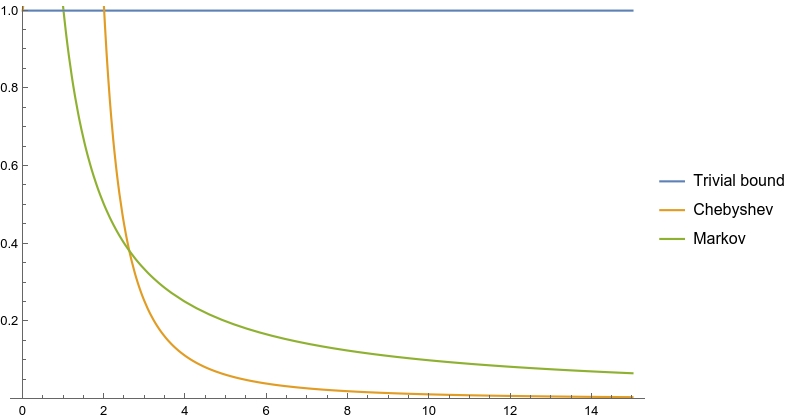
\includegraphics[width=0.9\textwidth]{figures/fig-markov-v-chebyshev.png}
    \caption{An illustration of the tail bounds $\probaOf{X\geq t}$ (as a function of $t\geq 0$) given by Markov and Chebyshev's inequalities, for the specific case of a non-negative random variable $X\geq 0$ with both expectation and variance equal to $1$: $\expect{X}=\var[X]=1$. Note that Chebyshev does not require that $X\geq 0$, this is simply here for the sake of comparison with Markov's inequality, which does.}
    \label{fig:markov:chebyshev}
\end{figure}
So we want to use Chebyshev's inequality to argue $\probaOf{X \leq \frac{\orange{m}}{2} - \Delta}$ is small. Here we go: rewriting $\frac{\orange{m}}{2} - \Delta = \expect{X} - \left(\Delta - \frac{\orange{m}}{2\ns}\right)$ and using $\orange{m}\leq \ns$ (so $\Delta - \frac{\orange{m}}{2\ns} \geq \Delta - \frac{1}{2} \geq \frac{\Delta}{2} = 2\sqrt{\orange{m}}$), we have
\begin{align*}
    \probaOf{X \leq \frac{\orange{m}}{2} - \Delta}
    &= \probaOf{X \leq \expect{X} - \left(\Delta - \frac{\orange{m}}{2\ns}\right)}\\
    &\leq \probaOf{\abs{X-\expect{X}} \geq \left(\Delta - \frac{\orange{m}}{2\ns}\right)}\\
    &\leq \frac{\var[X]}{\big(\Delta - \frac{\orange{m}}{2\ns}\big)^2} \tag{by Chebyshev}\\
    &\leq \frac{\orange{m}}{4(\Delta/2)^2} \tag{Bound on variance}\\
    &= \frac{1}{16} \tag{Setting of $\Delta$} 
\end{align*}
This gives us
\begin{equation}
    \label{eq:bounding:approxmedians:1}
    \probaOf{E_1},\probaOf{E_2} \leq \frac{1}{16}\,,
\end{equation}
using Chebyshev's inequality. We only have to bound $\probaOf{E_3}$ to conclude.

\paragraph{Bounding $\probaOf{E_3}$.} This is the last piece:\footnote{For now at last: there will be more down the line.} we want to bound the probability that $\blue{C}$ is ``too large,'' that is the probability $|\blue{C}|$ exceeds $4\orange{m}$. Since all we have seen so far relies either on computing the expectation of the quantity of interest, its variance, or both, it would seem reasonable to start with computing $\expect{|\blue{C}|}$ and maybe use Markov's inequality: unfortunately,
the quantity $\expect{|\blue{C}|}$ is quite tricky to compute. 

Instead, we will take an alternative path: let $R_{\underline{b}}$ denote the rank of $\underline{b}$ in $\red{A}$ (and similarly $R_{\overline{b}}$ for $\overline{b}$). We have already proven that 
\[
\probaOf{ R_{\underline{b}} > \frac{\ns}{2}} , \probaOf{ R_{\overline{b}} < \frac{\ns}{2}} \leq \frac{1}{16}
\]
(this is~\cref{eq:bounding:approxmedians:1}). Now, we want to prove that $|\blue{C}| = R_{\overline{b}}-R_{\underline{b}} +2 \leq \frac{4\ns\Delta}{\orange{m}}+2$ with high probability: so it'd \emph{suffice} to show that 
\[
\probaOf{ R_{\underline{b}} < \frac{\ns}{2} - 2\frac{\ns\Delta}{\orange{m}}} , \probaOf{ R_{\overline{b}} > \frac{\ns}{2} + 2\frac{\ns\Delta}{\orange{m}}} \leq \frac{1}{32}
\]
as this would imply the result. One may ask: \emph{why these particular values?} The reason is that since $\underline{b}$ is defined as the ($\frac{\orange{m}}{2} - \Delta$)-th element in $\orange{B}$, if the uniform random sampling was ``representative'' enough we expect to have an $\frac{1}{2} - \frac{\Delta}{\orange{m}}$ fraction of the original array $\red{A}$ on its left: so having much less than that, say a fraction $\frac{1}{2} - 2\frac{\Delta}{\orange{m}}$, ``should'' be unlikely.

As before, we will only focus on bounding $\probaOf{ R_{\underline{b}} < \frac{\ns}{2} - 2\frac{\ns\Delta}{\orange{m}}}$, as the case of $R_{\overline{b}}$ is similar (by symmetry). 

To proceed, let's consider the set $S$ of the $s\eqdef \frac{\ns}{2} - 2\frac{\ns\Delta}{\orange{m}}$ smallest elements of $\red{A}$~--~let's call them ``tail elements''. The key observation is that if \emph{fewer} than $\frac{\orange{m}}{2}-\Delta$ elements of $S$ end up in $\orange{B}$, then $\underline{b}$, being the ($\frac{\orange{m}}{2}-\Delta$)-th element of $\orange{B}$, is not a tail element: and so must have $R_{\underline{b}} \geq s$. Based on that, we want to show that the probability to have \emph{at least} $\frac{\orange{m}}{2}-\Delta$ of $S$ in $\orange{B}$ is small.

Now this looks familiar: the probability to pick an element of $S$ when choosing one from $\red{A}$ uniform at random is $\frac{s}{\ns} = \frac{1}{2} - \frac{2\Delta}{\orange{m}}$. The number of elements from $S$ in $\orange{B}$ (call it $Y$) is then a Binomial random variable with parameters $\orange{m}$ and $\frac{s}{\ns}$. We have $\expect{Y} = \frac{\orange{m}s}{\ns} = \frac{\orange{m}}{2}-2\Delta$, $\var[Y] = \frac{\orange{m}s}{\ns}\Paren{1-\frac{s}{\ns}} \leq \frac{\orange{m}s}{\ns} \leq \frac{\orange{m}}{2}$; and we want to bound
\begin{align*}
    \probaOf{Y \geq \frac{\orange{m}}{2}-\Delta}
    &= \probaOf{Y \geq \expect{Y}+\Delta} \\
    &\leq  \probaOf{|Y - \expect{Y}| \geq \Delta} \\
    &\leq \frac{\var[Y]}{\Delta^2} \tag{Chebyshev}\\
    &= \frac{\orange{m}}{2\cdot 16\orange{m}} \tag{as $\Delta= 4\sqrt{\orange{m}}$}\\
    &= \frac{1}{32}
\end{align*}
To summarize, we've just shown that
\[
    \probaOf{ R_{\underline{b}} < \frac{\ns}{2} - 2\frac{\ns\Delta}{\orange{m}}} \leq \probaOf{Y \geq \frac{\orange{m}}{2}-\Delta} \leq \frac{1}{32}
\]
We can similarly get $\probaOf{ R_{\overline{b}} > \frac{\ns}{2} + 2\frac{\ns\Delta}{\orange{m}}} \leq \frac{1}{32}$\marginnote{Do it! That's good practice.}, and so, ``by a union bound,''
\begin{align}
    \probaOf{E_3} &= \probaOf{|\blue{C}| > \frac{4\ns\Delta}{\orange{m}} + 2} \notag\\
    &\leq \probaOf{ R_{\underline{b}} < \frac{\ns}{2} - 2\frac{\ns\Delta}{\orange{m}}} + \probaOf{ R_{\overline{b}} > \frac{\ns}{2} + 2\frac{\ns\Delta}{\orange{m}}} \notag\\
    &\leq \frac{1}{16}\,.
\end{align}

\paragraph{Putting it together.}
The probability that the algorithm fails is bounded, from~\cref{eq:first:union:bound}, by
\[
\probaOf{E_1\cup E_2\cup E_3} \leq \probaOf{E_1}+\probaOf{E_2}+\probaOf{E_3} \leq \frac{1}{16} + \frac{1}{16} + \frac{1}{16} = \frac{3}{16}\,.
\]
When it doesn't fail, we have seen that it is correct; and it \emph{always} runs in time at most $O(\ns)$. So\dots{} we're done! \emph{Almost.} We haven't chosen the value of $\orange{m}$ yet!

So what do we need? For our running time, we need both $O(\orange{m}\log\orange{m})$ and $O(\frac{\ns\Delta}{\orange{m}}\log\frac{\ns\Delta}{\orange{m}}) =O(\frac{\ns}{\sqrt{\orange{m}}}\log \frac{\ns}{\sqrt{\orange{m}}})$ to be $O(\ns)$. There are many ways to do so, but one aesthetically pleasing choice is to make both equal:
\[
    \orange{m} = \frac{\ns}{\sqrt{\orange{m}}}
\]
which leads to setting $\boxed{\orange{m} = \ns^{2/3}}$. To conclude:
\begin{theorem}
    \label{theo:randomized:median}
    Randomised Median (\cref{algo:randomized:median}) is a linear-time Monte Carlo algorithm with failure probability at most $3/16$.
\end{theorem}

\section{But can we bring down this failure probability?}
This is all very good, but, when you think about it, a failure probability of $3/16\approx 19\%$ might be too much for many applications. Can we somehow bring this down to $1\%$? $0.01\%$? $\errprob$, for any $\errprob\in(0,1]$ of our choosing?

The obvious natural approach would be to go back to our analysis, see what the bottlenecks were, and modify the parameters to achieve smaller error probability. This would work \emph{here}\marginnote{\advancedstuff{} Go through the argument and see what happens to the probability of failure when you choose a larger $\Delta$, for instance $\orange{m}^{3/4}$ or $\sqrt{\ns}$.}, but it may not \emph{always} work, and honestly it is also very inconvenient. We went through a lot of trouble to establish~\cref{theo:randomized:median}, it would be nice not to have to start all over again!

Fortunately, it \emph{is} possible: there is a way to take our algorithm (and the guarantees we proved for it), and amplify its success probability \emph{in a blackbox way}. Of course, there is a cost: we will need to run the algorithm several times~--~the price is more computation time, and more random bits.\marginnote{Random bits are not always cheap: they are a resource, like time, and memory.}

Here is the idea: given the input array $\red{A}$ run the algorithm (\cref{algo:randomized:median}) $T$ times on $\red{A}$, using fresh (independent) random bits each time. If at any point the algorithm does not return $\textsf{fail}$, then return the median it outputs. If this never happens, return $\textsf{fail}$.

Since we have a Monte Carlo algorithm, whenever we return something else than $\textsf{fail}$ this is guaranteed to be correct, and we have the median. So what is the probability to output $\textsf{fail}$ now? Well, we need \emph{all} $T$ independent runs to fail. And they are all independent, so the probability that they all fail is at most
\[
    \Paren{\frac{3}{16}}^T
\]
Solving for this to be less than $\errprob$, we get that  taking
\[
    T = \clg{\frac{\log(1/\errprob)}{\log\frac{16}{3}}} = O(\log(1/\errprob))
\]
suffices. This gives the following:
\begin{corollary}
    \label{coro:randomized:median}
    For any $\errprob \in(0,1]$, the Repeated Randomised Median described above is a Monte Carlo algorithm with failure probability at most $\errprob$ and worst-case time complexity $O(\ns\log(1/\errprob))$.
\end{corollary}
\noindent This simple ``trick'' is your first example of \emph{probability amplification.}

\section{Viva Las Vegas!}
In light of~\cref{coro:randomized:median}, it is natural to wonder: why stopping there? Can we convert any Monte Carlo algorithm into a Las Vegas algorithm, providing a converse to~\cref{lemma:lvtomc}?

The answer is \emph{not always} (not for every Monte Carlo algorithm), but in this particular case yes. The key observation is that~\cref{algo:randomized:median} is not \emph{any} Monte Carlo algorithm: it never ``fail silently.'' That is, when the \cref{algo:randomized:median} fails, it tells us so! This is a very valuable feature.

Consider the following algorithm:
\begin{algorithm}[H]
\begin{algorithmic}[1]
    \Require array $\red{A}$ of $\ns$ distinct integers
    \Repeat
        \State Run~\cref{algo:randomized:median} on $\red{A}$ (with fresh random bits)
        \State Let $y$ be the output
    \Until{$y\neq \textsf{fail}$}\label{step:until:exit}
    \State\Return $y$
\end{algorithmic}
    \caption{Randomised Median in Expected Linear Time.}
    \label{algo:randomized:median:lv}
\end{algorithm}
Correctness is immediate: whenever this new algorithm stops, the $y$ it outputs is the median of $\red{A}$. But \emph{does it ever stop}? And if so, what is its expected running time?\medskip

Let $\tau(\ns) = O(\ns)$ be the (worst-case) running time of \cref{algo:randomized:median}, and $K$ be the (random) number of loop iterations before~\cref{algo:randomized:median:lv} terminates. Clearly, the (random) running time of~\cref{algo:randomized:median:lv} is (at most) $K\cdot \tau(\ns)$. What can we say about $K$?\marginnote{Some vocabulary: $K$ as defined here is a \emph{geometric random variable} with parameter $p \geq 13/16$.}
\begin{enumerate}
    \item The probability that $K\geq 1$ is $1$: we always run the loop at least once.
    \item The probability that $K\geq 2$ is at most $3/16$: to go to the second iteration of the loop, the first call to~\cref{algo:randomized:median} must have failed.
    \item The probability that $K\geq 3$ is at most $(3/16)^2$: to go to the third iteration of the loop, the first two calls to~\cref{algo:randomized:median} must have failed (and they are independent).
    \item The probability that $K\geq k$ is at most $(3/16)^{k-1}$: to go to the $k$-th iteration of the loop, the first $k-1$ calls to~\cref{algo:randomized:median} must have failed (and they are independent).
\end{enumerate}
This is particularly useful, since from what we say in the first chapter we can write
\[
    \expect{K} = \sum_{k=1}^\infty \probaOf{K\geq k} 
\]
and here this becomes
\[
    \expect{K} \leq \sum_{k=1}^\infty \Paren{\frac{3}{16}}^{k-1} = \frac{16}{13} \leq  1.231
\]
This means that the expected running time of our Las Vegas algorithm,~\cref{algo:randomized:median:lv}, is at most $1.231\cdot \tau(\ns) = O(\ns)$!
\begin{corollary}
    \label{coro:randomized:median:lv}
    For any $\errprob \in(0,1]$, the Indefinitely Repeated Randomised Median (\cref{algo:randomized:median:lv}) is a Las Vegas algorithm with expected time complexity $O(\ns)$.
\end{corollary}
\noindent More generally, we can prove the following:
\begin{theorem}
    Let $\Algo$ be a Monte Carlo algorithm with worst-case running time $T(\ns)$ and constant failure probability $p\in(0,1)$, with the following extra guarantee: one can detect whether the output of $\Algo$ is incorrect in time $O(1)$. Then there exists a \emph{Las Vegas} algorithm $\Algo'$ for the same task with expected running time $O(T(\ns))$ (where the hidden constant in the $O(\cdot)$ depends on $p$).
\end{theorem}
\begin{proof}
    Your turn!
\end{proof}

\section{And to conclude, something totally different!}\marginnote{Probability amplification by Majority Vote}
The Randomised Median algorithm we saw (\cref{algo:randomized:median}) was quite nice, as far as Monte Carlo algorithms go: whenever it failed, \emph{it told us so.}
But that's usually not the case. Consider for instance the following scenario: someone implemented a very useful thing, say a data structure with its API, and gives you access. You cannot see the code or the implementation to check it's correct: all you can do is query that data structure $\red{D}$, and on input element $\blue{x}$ this query $\green{\mathcal{Q}}$ to $\red{D}$ is supposed to output
\[
    \green{\mathcal{Q}}(\blue{x}) = \begin{cases}
        \yes &\text{if } \blue{x}\in\red{D} \\
        \no &\text{if } \blue{x}\notin\red{D} \\
    \end{cases}
\]
Unfortunately, the implementation is \emph{not} correct, or something is wrong: for whatever reason, each query behaves somewhat randomly, and is only correct with probability $60\%$.\marginnote{This sounds ridiculous? Wait until you hear about hashing and Bloom filters later in the course.} And when it's wrong, of course, you don't know it!

\begin{framed}
    Can we use this data structure access in a blackbox way to obtain better guarantees, and have queries that are correct with probability $99\%$ instead? Probability $1-\errprob$?
\end{framed}

The answer is, again, \emph{yes}. And the probability amplification technique to use here is very intuitive: a simple \emph{majority vote}. Here's what we will do, where $T=T(\errprob)$ is an integer to be determined shortly:
\begin{algorithm}[H]
\begin{algorithmic}[1]
    \Require blackbox access to $\red{D}$ via $\green{\mathcal{Q}}$; input $\blue{x}$
    \For{$t=1,2,\dots, T$}
        \State $y_t \gets \green{\mathcal{Q}}(\blue{x}) \in\{\yes,\no\}$
    \EndFor
    \State\Return $\operatorname{majority}(y_1,\dots,y_T)$ \Comment{$\yes$ if at least half of the $y_t$'s are $\yes$}
\end{algorithmic}
    \caption{More reliable data structure via majority vote.}
    \label{algo:majority:vote}
\end{algorithm}
Let us analyze this. For any fixed $\blue{x}$, we know that each $y_t\in\{0,1\}$ is the correct answer with probability at least $6/10$, and are independent (we assume that the random errors are independent, at least). So if we define
\[
    Y = \sum_{t=1}^T \indic{y_t\text{ is correct}}
\]
we have a sum of independent Bernoulli random variables.\marginnote{It's even a Binomial r.v. with parameters $T$ and $p\geq 6/10$, but we will not need to be that precise.} And since we take a majority vote, the only way for our output to be incorrect is to have \emph{more than half} of the $T$ answers being incorrect, that is, to have $Y < \frac{1}{2}T$.

But $\expect{Y} \geq \frac{6}{10}T$, so to be wrong we need $Y$ to be more than $\frac{1}{10}T$ away from its expectation. This should ring a bell: \emph{we can use Chebyshev's inequality for that!}\smallskip

We \emph{could}, but that will not be good enough (that won't give a good enough bound).\marginnote{Try it: Chebyshev should get you something like $\probaOf{Y < \frac{1}{2}T} \leq \frac{24}{T}$.} We can do better! 
Enters the \emph{Chernoff bound}:
\begin{theorem}[Chernoff bound]
Let $X_1,\dots,X_n$ be \emph{independent} random variables taking value in $[0,1]$, and let $P \eqdef \sum_{i=1}^n \bEE{X_i}$ For any $\gamma \in (0,1]$ we have
\begin{align}
\bPr{\sum_{i=1}^n X_i > (1+\gamma)P } &< \exp(-\gamma^2 P/3)\\
\bPr{\sum_{i=1}^n X_i < (1-\gamma)P } &< \exp(-\gamma^2 P/2)
\end{align}
\end{theorem}
We can apply it with ``$n=T$, $P=\frac{6}{10}T$, and $\gamma=\frac{1}{6}$'' (the last one to have $(1-\gamma)\cdot \frac{6}{10}T = \frac{1}{2}T$), and that immediately gives us
\[
    \bPr{ Y < \frac{1}{2}T } \leq e^{-\frac{1}{120}T}
\]
which decays \emph{exponentially} with $T$.\marginnote{Sure, the constant $1/120$ in there is not great, but we could do better by sweating a bit more.} In particular, for large $T$ this is much, much better than what Chebyshev would give:
\begin{figure}
    \centering
    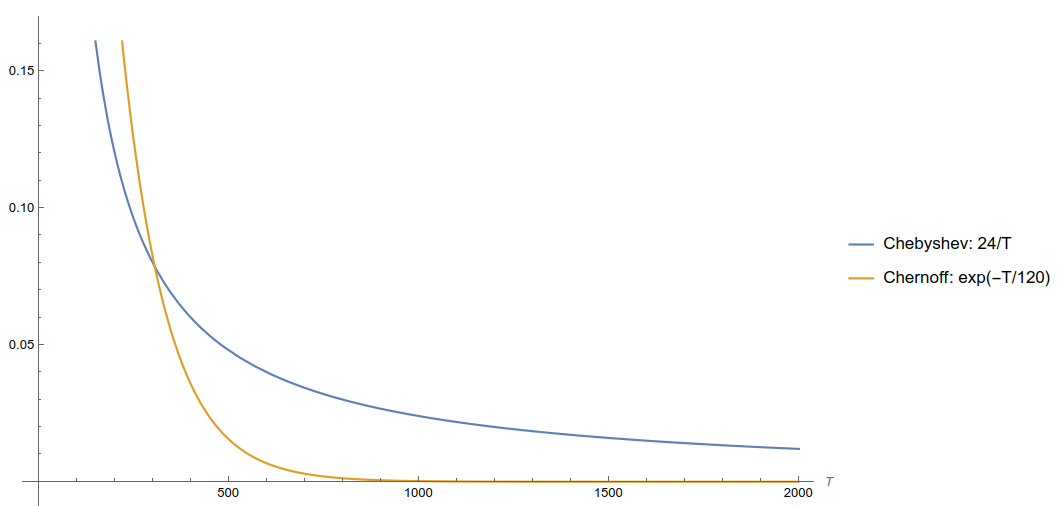
\includegraphics[width=1.25\textwidth]{figures/fig-chernoff-v-chebyshev.png}
    \caption{Bounds on $\bPr{ Y < \frac{1}{2}T }$ provided by Chebyshev's and Chernoff's inequalities, as a function of $T$.}
    \label{fig:chernoff:v:chebyshev}
\end{figure}
In any case: we wanted a failure probability less than $\errprob$? Then is suffices to solve for (integer) $T$:
\[
e^{-\frac{1}{120}T} \leq \errprob
\]
giving $T \geq \clg{120\ln(1/\errprob)}$. So with taking $T(\errprob)=O(\log(1/\errprob))$ in~\cref{algo:majority:vote} suffices to amplify the success probability of each query on $\blue{x}$ from $60\%$ to $1-\errprob$, at the (small?) cost of $O(\log(1/\errprob))$ more queries to the data structure $\red{D}$.

\begin{framed}
 We have used Markov's and Chebyshev's inequalities and the Chernoff bound, and this allowed us to analyse and amplify the success probability of our randomised algorithms. In the next lectures, we will see a related technique, also based on the Chernoff (or, looking ahead, Hoeffding) bound: a generalisation of the ``majority vote'' trick for when the output can take more than only 2 values, called the \emph{median trick.}
\end{framed}


\section{Concentration inequalities: a summary}
We summarize the ``concentration bounds''\marginnote{They are called that way because they quantify how ``concentrated'' (in terms of probability) a random variable is around its expectation.} used in the chapter so far, along with some others (more advanced) that will come in handy in the next chapters. These will be sufficient in many or most settings. 
There are, of course, \emph{many} others, and many refinements or variants of the bounds we present here. If you are interested, see \eg Chapter~2 of \cite{Vershynin18} or~\cite{BoucheronLM13} for a much more comprehensive and insightful coverage.

We start with the mother of all concentration inequalities, Markov's inequality:
\begin{theorem}[Markov's inequality]
  \label{theo:markov}
Let $X$ be a non-negative random variable with $\bEE{X} < \infty$. For any $t > 0$, we have
\[  
  \bPr{ X \geq t } \leq \frac{\bEE{X}}{t}
\]
\end{theorem}
\noindent Applying this to $(X-\bEE{X})^2$, we get 
\begin{theorem}[Chebyshev's inequality]
  \label{theo:chebyshev}
Let $X$ be a random variable with $\bEE{X^2} < \infty$. For any $t > 0$, we have
\[  
  \bPr{ \abs{X-\bEE{X}} \geq t } \leq \frac{\var[X]}{t^2}
\]
\end{theorem}
By applying Markov's inequality to the moment-generating function (MGF) of $\sum_{i=1}^n X_i$ in various ways, one can also obtain the following statements:
\begin{theorem}[Hoeffding bound]
  \label{theo:hoeffding}
Let $X_1,\dots,X_n$ be independent random variables, where $X_i$ takes values in $[a_i,b_i]$. For any $t \geq 0$, we have
\begin{align}
\bPr{ \sum_{i=1}^n X_i   > \sum_{i=1}^n \bEE{X_i} + t }  
&\leq \exp(-\frac{2 t^2}{\sum_{i=1}^n (b_i-a_i)^2}) \\
\bPr{\sum_{i=1}^n X_i  < \sum_{i=1}^n \bEE{X_i} - t }
 &\leq \exp(-\frac{2 t^2}{\sum_{i=1}^n (b_i-a_i)^2})
 \end{align}
\end{theorem}

\begin{corollary}[Hoeffding bound]
  \label{coro:hoeffding}
Let $X_1,\dots,X_n$ be \iid random variables taking value in $[0,1]$, with mean $\mu$. For any $\gamma \in (0,1]$ we have
\begin{align}
\bPr{ \abs{\frac{1}{n}\sum_{i=1}^n X_i  - \mu} > \gamma }
 &\leq 2\exp(-2 \gamma^2 n)
\end{align}
\end{corollary}

\begin{theorem}[Chernoff bound]
  \label{theo:chernoff}
Let $X_1,\dots,X_n$ be independent random variables taking value in $[0,1]$, and let $P \eqdef \sum_{i=1}^n \bEE{X_i}$ For any $\gamma \in (0,1]$ we have
\begin{align}
\bPr{\sum_{i=1}^n X_i > (1+\gamma)P } &< \exp(-\gamma^2 P/3)\\
\bPr{\sum_{i=1}^n X_i < (1-\gamma)P } &< \exp(-\gamma^2 P/2)
\end{align}
In particular, if $X_1,\dots,X_n$ are \iid with mean $\mu$, then for any $\gamma \in (0,1]$ we have
\begin{align}
\bPr{ \abs{\frac{1}{n}\sum_{i=1}^n X_i  - \mu} > \gamma\mu }
 &\leq 2\exp(-\gamma^2 n \mu/3) \label{eq:chernoff:iid}
\end{align}
\end{theorem}
As a rule of thumb, the ``multiplicative'' (Chernoff) from~\cref{theo:chernoff} is preferable to the ``additive'' bound (Hoeffding) from~\cref{coro:hoeffding} whenever $\mu  \eqdef P/n \ll 1$. In case one only has an upper or lower bound on the quantity $P = \sum_{i=1}^n \bEE{X_i}$, the following version of the Chernoff bound can come in handy:
\begin{theorem}[Chernoff bound (upper and lower bound version)]
  \label{theo:chernoff:with:ublb}
In the setting of~\cref{theo:chernoff}, suppose that
$P_L \leq P \leq P_H.$ Then for any $\gamma \in (0,1]$, we have
\begin{align}
\bPr{\sum_{i=1}^n X_i > (1+\gamma)P_H } &< \exp(-\gamma^2 P_H/3) \\
\bPr{\sum_{i=1}^n X_i < (1-\gamma)P_L } &< \exp(-\gamma^2 P_L/2)
\end{align}
\end{theorem}

%%%%%%%%%%%%%%%%%%%%%%%%%%%%%%%%%%%%%%%%%%%%%%%%%%%%%%%%%%%%%%%
\iffalse
\begin{theorem}[Bernstein's inequality] \label{theo:bernstein}
	Let $X_1,\dots, X_n$ be independent random variables taking values in $[-a,a]$, and such that $\bEE{X_i^2} \leq v_i$ for all $i$. Then, for every $t\geq 0$, we have
	\[
	\bPr{ \abs{\sum_{i=1}^n X_i-\sum_{i=1}^n \bEE{X_i}} \geq t } \leq \exp\Paren{-\frac{t^2}{2(\sum_{i=1}^n v_i+\frac{a}{3}t)}}\,.
	\]
	In particular, if $X_1,\dots,X_n$ are \iid with mean $\mu$ and $\bEE{X_1^2} \leq v$, then for any $\gamma \geq 0$ we have
	\[
	\bPr{ \abs{\frac{1}{n}\sum_{i=1}^n X_i-\mu} \geq \gamma } \leq \exp\Paren{-\frac{\gamma^2n}{2(v+\frac{a}{3}\gamma)}}\,.
	\]
\end{theorem}
Observe that this tail bound exhibits both behaviours: it decays in a subgaussian fashion for small $\gamma$, before switching to a subexponential tail bound for large $\gamma$. 

We conclude this section by providing a very convenient bound, specifically for Poisson random variables, which shares the same ``two-tail'' behaviour:
\begin{theorem}[Poisson concentration]\label{theo:main:poisson:bounds}
Let $X$ be a $\poisson{\lambda}$ random variable, where $\lambda > 0$. Then, for any $t>0$, we have
\begin{equation}\label{eq:poisson:upper:tail}
    \probaOf{ X \geq \lambda + t} \leq e^{-\frac{t^2}{2\lambda}\psi\Paren{\frac{t}{\lambda}}} \leq e^{-\frac{t^2}{2(\lambda+t)}}
\end{equation}
and, for any $0<t< \lambda$,
\begin{equation}\label{eq:poisson:lower:tail}
  \probaOf{ X \leq \lambda - t} \leq e^{-\frac{t^2}{2\lambda}\psi\Paren{-\frac{t}{\lambda}}} \leq e^{-\frac{t^2}{2(\lambda+t)}}\,,
\end{equation}
where $\psi(u)\eqdef 2\frac{(1+u)\ln(1+u)-u}{u^2}$ for $u\geq -1$.
In particular, for any $t\geq 0$,
\begin{equation}\label{eq:poisson:both:tail}
  \probaOf{ \abs{X -\lambda} \geq t} \leq 2e^{-\frac{t^2}{2(\lambda+t)}}\,.
\end{equation}
\end{theorem}
\cmargin{Is the proof needed?}
\fi

\chapter{Lecture 3: Balls in Bins}
You have $\nballs$ balls, and want to randomly distribute them among $\nbins$ different bins. Why? That's a pretty good question: basically, and you'll have to believe me for now, this rather strange scenario (and its many variants) capture a lot of actual interesting or well-motivated problems.\marginnote{We'll get back to those.}

The things we might care about are (1)~the \emph{maximum load} of the bins, that is, what's the maximum number of balls any given bin contains once we've distributed them; (2)~the \emph{coverage}, that is, how many bins are non-empty; and (3)~the \emph{collisions}, that is, how many pairs of distinct balls share the same bin.

The simplest thing we can do is throwing our $\nballs$ into the $\nbins$ independently and uniformly at random. Let's see how that goes.

\section{Collisions}
One of the most basic things we can ask is whether the $\nballs$ balls will all fall into their own personal bin, that is, if there's going to be at least one bin containing more than one ball. \emph{What's the probability to get at least one collision?}

\paragraph{Interlude:} \emph{run the Birthday Paradox experiment in the classroom. Discuss assumptions (uniformity), etc.}

\begin{theorem}[Birthday Paradox]
If you gather 23 people in a room, then with probability 50\% there will be two sharing a birthday.
\end{theorem}

To prove that, we'll tackle the more general question, for arbitrary $\nballs$ and $\nbins$, of finding what the probability $p_{\nballs, \nbins}$ of having at least one collision is: the birthday paradox is for $\nbins=366$, because, of course, 2024 is a leap year\marginnote{That might change in 2025...}, and asks to check that $p_{23,366} \geq 1/2$. Now, the result has to depend on the relation between $\nballs$ and $\nbins$: if $\nballs \geq \nbins + 1$, then that probability is exactly one,\marginnote{Do you see why? Prove it (Pigeonhole).} while if $\nbins \gg \nballs$ this should be less likely.

\begin{theorem}
    \label{theo:collisions:pnm}
    The probability $p_{\nballs, \nbins}$ to get at least one collision is equal to
    \begin{equation}
        \label{eq:collisions:pnm}
        p_{\nballs, \nbins} = 1 - \frac{\nbins!}{\nbins^{\nballs}(\nbins-\nballs)!} = 1 - \frac{\nballs!}{\nbins^{\nballs}} \binom{\nbins}{\nballs}
    \end{equation}
    In particular, for $\nballs = 23$ and $\nbins=366$, this is...?\marginnote{Check it: $p_{22,366} \approx 0.475$, while $p_{23,366} \approx 0.506$.}
\end{theorem}
\begin{proof}
    \begin{align*}
    1-p_{\nballs, \nbins} &= \frac{\nbins}{\nbins}\cdot\frac{\nbins-1}{\nbins}\cdot \frac{\nbins-2}{\nbins}\cdots \frac{\nbins-\nballs+1}{\nbins}
    = \frac{1}{\nbins^{\nballs}}\prod_{\ell=0}^{\nballs-1} (\nbins-\ell) \\
    &= \frac{\nbins!}{\nbins^{\nballs}(\nbins-\nballs)!} 
    \end{align*}
\end{proof}
\begin{figure}[htbp]
    \centering
    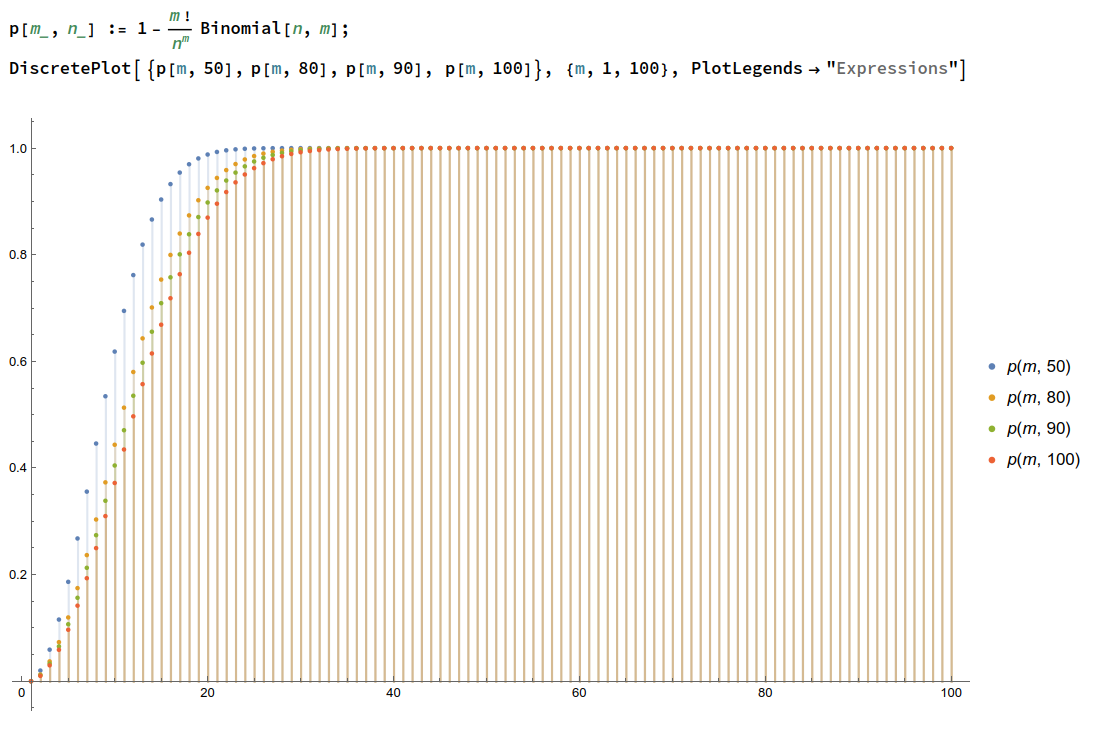
\includegraphics[width=1.0\textwidth]{figures/fig-collisions-nm.png}
    \caption{The quantity $p_{\nballs, \nbins}$ from~\cref{eq:collisions:pnm}, plotted here as a function of $\nballs$ for various choices of $\nbins$.}
    \label{fig:collisions:nm}
\end{figure}

Looking at the graph above, it looks like we approach a very high probability of getting a collision \emph{way} before $\nballs = \Theta(\nbins)$. Any guess at what $\nballs$ should be to, say, have probability at least $50\%$ of a collision? Should it be
\begin{itemize}
    \item $\Theta(\log\nbins)$?
    \item $\Theta(\sqrt{\nbins})$?
    \item $\Theta\Paren{\frac{\nbins}{\log\nbins}}$?
    \item Something else?
\end{itemize}
And \emph{why}?

\paragraph{The worst approach: rabbit-out-of-a-hat, no intuition given.} Take $\nballs = c\cdot\sqrt{\nbins}$ for some fixed constant $c>0$. Plugging this in the expression $p_{\nballs,\nbins}$ obtained in~\cref{theo:collisions:pnm}, we get
\begin{align*}
1 - p_{\nballs,\nbins} = \frac{\nbins!}{\nbins^{\nballs}(\nbins-\nballs)!}
&\operatorname*{\sim}_{\nbins\to\infty} 
\frac{1}{\nbins^{\nballs}}\cdot \frac{\sqrt{2\pi \nbins} \Paren{\frac{\nbins}{e}}^{\nbins}}{\sqrt{2\pi(\nbins-\nballs)}\Paren{\frac{\nbins-\nballs}{e}}^{\nbins-\nballs}} \tag{Stirling} \\
&= \frac{1}{\sqrt{1-\frac{\nballs}{\nbins}}} \frac{ \nbins^{\nbins-\nballs}}{\Paren{\nbins-\nballs}^{\nbins-\nballs} e^{\nballs}} \tag{``Massaging''}\\
&= \frac{1}{\sqrt{1-\frac{\nballs}{\nbins}}} \frac{1}{\Paren{1-\frac{\nballs}{\nbins}}^{\nbins-\nballs} e^{\nballs}} \\
&= \frac{1}{\sqrt{1-\frac{\nballs}{\nbins}}} \frac{1}{\Paren{1-\frac{\nballs}{\nbins}}^{\nbins} e^{\nballs}} \cdot \Paren{1-\frac{\nballs}{\nbins}}^{\nballs} \\
&= \frac{1}{\sqrt{1-\frac{c}{\sqrt{\nbins}}}} \frac{1}{\Paren{\Paren{1-\frac{c}{\sqrt{\nbins}}}^{\sqrt{\nbins}} e^{c}}^{\sqrt{\nbins}}} \cdot \Paren{1-\frac{c}{\sqrt{\nbins}}}^{c\sqrt{\nbins}} \tag{Finally!}
\end{align*}
the last line using our choice of $\nballs$. From there, ``all'' that remains to check is that $\lim_{\nbins\to\infty} \sqrt{1-\frac{c}{\sqrt{\nbins}}} = 1$ (easy), that 
\[
\lim_{\nbins\to\infty} \Paren{\Paren{1-\frac{c}{\sqrt{\nbins}}}^{\sqrt{\nbins}} e^{c}}^{\sqrt{\nbins}} = e^{-c^2/2}
\] (less easy)\marginnote{Do it!}, and that
\[
\lim_{\nbins\to\infty} \Paren{1-\frac{c}{\sqrt{\nbins}}}^{c\sqrt{\nbins}} = e^{-c^2}
\]
(not too hard?) to conclude that
\begin{align*}
1 - p_{c\sqrt{\nbins},\nbins} 
&\operatorname*{\sim}_{\nbins\to\infty} 1\cdot \frac{1}{e^{-c^2/2}} \cdot e^{-c^2} = e^{-c^2/2} 
\end{align*}
or, equivalently,
\begin{align*}
p_{c\sqrt{\nbins},\nbins} 
= 1 - e^{-c^2/2} +o(1)
\end{align*}
This shows that the probability to get a collision becomes constant for $\nballs = \Theta(\sqrt{\nbins})$.
Now, that's nice, but you may ask yourself, \emph{``Well, how did I get here?''}

\paragraph{Let's take a step back.} So we throw $\nballs$ balls into $\nbins$ bins. Let's start with the simplest case possible: let's throw \emph{two} balls into $\nbins$. What's the probability that they end up in the same bin?\marginnote{Don't look immediately! Think about it first.}\clearpage

The first ball falls into a given bin, say the $i$-th. Then to get a collision the second ball has to be thrown into the same bin $i$, which happens with probability $1/\nbins$. So $p_{2,\nbins} = 1/\nbins$. A more verbose way to derive it is as follows: let $\red{X_1}, \blue{X_2}$ denote the indices of the bins $\bin$ for the first $\balla$ and second $\ballb$ ball, respectively. These are independent r.v.'s, uniformly distributed in $[\nbins]$, so
\begin{align}
p_{2,\nbins} &= \probaOf{\red{X_1}=\blue{X_2}} = \sum_{k=1}^{\nbins} \probaOf{\red{X_1}=k, \blue{X_2}=k} \notag\\
&= \sum_{k=1}^{\nbins} \probaOf{\red{X_1}=k}\cdot\probaOf{\blue{X_2}=k} \notag\\
&= \sum_{k=1}^{\nbins} \frac{1}{\nbins}\cdot\frac{1}{\nbins} = \frac{\nbins}{\nbins^2} = \frac{1}{\nbins} \,,
\end{align}
``as foretold.''

Back to the general $\nballs$ balls case. The above tells us that for every pair of balls, the probability to get a collision (ignoring all other balls) is $1/\nbins$. How many distinct pairs of balls do we have? Well, $\binom{\nballs}{2}$. So what's the \emph{expected} number of collisions $c(\nballs,\nbins)$?
\begin{align}
   c(\nballs,\nbins) 
   &= \expect{\sum_{(\red{i},\blue{j})\text{ pair}} \indic{\red{X_i} = \blue{X_j}} }\notag\\
   &= \sum_{(\red{i},\blue{j})\text{ pair}} \expect{\indic{\red{X_i} = \blue{X_j}} }\notag\\
   &= \sum_{(\red{i},\blue{j})\text{ pair}} \probaOf{\red{X_i} = \blue{X_j}} \notag\\
   &= \sum_{(\red{i},\blue{j})\text{ pair}} \frac{1}{\nbins} \notag\\
   &= \binom{\nballs}{2}\cdot\frac{1}{\nbins} \label{eq:expect:collisions}
\end{align}
where we used linearity of expectation, and our previous computation for the $\nballs=2$ case. This means that the expected number of collisions grows (roughly) as $\frac{\nballs^2}{2\nbins}$. If we believe that the number of collisions does not deviate too pathologically from its expected value, this becomes constant when $\nballs = \bigTheta{\sqrt{\nbins}}$. So we should start expecting collisions when $\nballs = \bigTheta{\sqrt{\nbins}}$, which explains (in hindsight) the result we got before!

But can we easily prove this ``intuition''? We have the expectation $c(\nballs,\nbins)$ of the number of collisions, we want to show that number (let's call this random variable $C$) does not deviate too far from its expectation. The most basic tools we've seen for this are Markov and Chebyshev's inequalities: here, we'll have to use Chebyshev.\marginnote{Do you see why?} So we need to compute the variance of our random variable $C$:
\[
C = \sum_{(\red{i},\blue{j})\text{ pair}} \indic{\red{X_i} = \blue{X_j}}
\]
where as before \red{$X_i$} is the index of the bin \bin where the \red{$i$}-th ball \ball lands, and $\indic{\red{X_i} = \blue{X_j}}$ is the indicator of the event \emph{``ball $\red{i}$ and ball $\red{j}$ collide.''}
We \emph{would like} to write that the variance of the sum is the sum of the variances (``linearity of variance''), something like this
\begin{align*}
\var[C] 
&= \var\left[\sum_{(\red{i},\blue{j})\text{ pair}} \indic{\red{X_i} = \blue{X_j}}\right] 
\stackrel{?}{=} \sum_{(\red{i},\blue{j})\text{ pair}} \var\left[\indic{\red{X_i} = \blue{X_j}}\right] \\
\end{align*}
which \emph{would} make our life so much easier, since then, using the variance of an indicator random variable (Bernoulli), we'd get
\[
\var[C] = \binom{\nballs}{2}\frac{1}{\nbins}\Paren{1-\frac{1}{\nbins}}
\]
Unfortunately, \emph{variance is not linear}: we could write the above $\stackrel{?}{=}$ equality \emph{if} the indicator variables $\indic{\red{X_i} = \blue{X_j}}$ were independent (across $(\red{i},\blue{j})$): \emph{and this is not the case here}.\marginnote{Do you see why they are not independent?}

And yet, since we are showing the bin (for each ball) \emph{uniformly} at random, some magic happens, and somehow the above expression is still true.\marginnote{In the proof below, locate exactly where we use the fact that the bin is chosen uniformly.}
\begin{lemma}[Well, actually\dots \advancedstuff]
\label{lemma:variance:collisions}
We have 
\[
\var[C] = \binom{\nballs}{2}\frac{1}{\nbins}\Paren{1-\frac{1}{\nbins}}
\]
\end{lemma}
\begin{proof}
    Since $\var[C] = \bEE{C^2} - \bEE{C}^2$ and we already have computed $\bEE{C}$, we only are missing the first term:
    \begin{align*}
        \bEE{C^2} &= \bEE{\left(\sum_{(\red{i},\blue{j})\text{ pair}} \indic{\red{X_i} = \blue{X_j}}\right)^2} \\
        &= \bEE{\sum_{(\red{i},\blue{j})\text{ pair}}\sum_{(\orange{k},\green{\ell})\text{ pair}} \indic{\red{X_i} = \blue{X_j}}\indic{\orange{X_k} = \green{X_\ell}}} \\
        &= \sum_{(\red{i},\blue{j})\text{ pair}}\sum_{(\orange{k},\green{\ell})\text{ pair}} \bEE{\indic{\red{X_i} = \blue{X_j}}\indic{\orange{X_k} = \green{X_\ell}}} \\
    \end{align*}
    This is a little intimidating to compute, but we can make the following observations about the summands:
    \begin{itemize}
        \item if the two pairs $(\red{i},\blue{j})$, $(\orange{k},\green{\ell})$ are the same,\footnote{When we consider pairs here, we don't care about ordering, so $(i,j)=(j,i)$.} then $\indic{\red{X_i} = \blue{X_j}}\indic{\orange{X_k} = \green{X_\ell}} = \indic{\red{X_i} = \blue{X_j}}^2 = \indic{\red{X_i} = \blue{X_j}}$, so
        \[
            \bEE{\indic{\red{X_i} = \blue{X_j}}\indic{\orange{X_k} = \green{X_\ell}}} 
            = \bEE{\indic{\red{X_i} = \blue{X_j}}} 
            = \frac{1}{\nbins}\,.
        \]
        There are exactly $\binom{\nballs}{2}$ such summands.
        \item if the two pairs $(\red{i},\blue{j})$, $(\orange{k},\green{\ell})$ are disjoint, then $\indic{\red{X_i} = \blue{X_j}}$, $\indic{\orange{X_k} = \green{X_\ell}}$ are independent, and so
        \[
            \bEE{\indic{\red{X_i} = \blue{X_j}}\indic{\orange{X_k} = \green{X_\ell}}} 
            = \bEE{\indic{\red{X_i} = \blue{X_j}}} \bEE{\indic{\orange{X_k} = \green{X_\ell}}} 
            = \frac{1}{\nbins^2}\,.
        \]
        There are exactly $\binom{\nballs}{2}\binom{\nballs-2}{2}$ such summands.
        \item else, then the two pairs $(\red{i},\blue{j})$, $(\orange{k},\green{\ell})$ are neither disjoint nor equal, then $|\{\red{i},\blue{j},\orange{k},\green{\ell}\}|=3$. For any such summand, $\indic{\red{X_i} = \blue{X_j}}\indic{\orange{X_k} = \green{X_\ell}}$ is of the form $\indic{\red{X_i} = \blue{X_j} = \orange{X_k}}$, and so
        \begin{align*}
            \bEE{\indic{\red{X_i} = \blue{X_j}}\indic{\orange{X_k} = \green{X_\ell}}} 
            &= \bEE{\indic{\red{X_i} = \blue{X_j} = \orange{X_k}}} \\
            &= \sum_{b=1}^{\nbins} \probaOf{\red{X_i} = b,  \blue{X_j} = b, \orange{X_k} = b} \\
            &= \frac{\nbins}{\nbins^3}\\
            &= \frac{1}{\nbins^2}\,.
        \end{align*}
        There are exactly $2\cdot \binom{3}{2}\binom{\nballs}{3} = 6\binom{\nballs}{3}$ such summands.\marginnote{Can you see why? (If that's any consolation, I am terrible at combinatorics.)}
    \end{itemize}
    As a sanity check, we do have $\binom{\nballs}{2} + \binom{\nballs}{2}\binom{\nballs-2}{2} + 6\binom{\nballs}{3} = \binom{\nballs}{2}^2$, so we did not miss any summand in the above distinction of cases. We can then rewrite
    \begin{align*}
        \bEE{C^2} 
        &= \binom{\nballs}{2}\cdot \frac{1}{\nbins}
        + \binom{\nballs}{2}\binom{\nballs-2}{2}\cdot \frac{1}{\nbins^2}
        + 6\binom{\nballs}{3}\cdot \frac{1}{\nbins^2} \\
        &= \binom{\nballs}{2}\cdot \frac{1}{\nbins} + \binom{\nballs}{2}^2\cdot \frac{1}{\nbins^2} - \binom{\nballs}{2}\cdot \frac{1}{\nbins^2} \tag{Magic?} \\
        &= \binom{\nballs}{2}\cdot \frac{1}{\nbins}\Paren{1-\frac{1}{\nbins}} + \binom{\nballs}{2}^2\cdot \frac{1}{\nbins^2} 
    \end{align*}
    That's really encouraging, since the second term is exactly $\bEE{C}^2$, and the first is what we were hoping to get for the variance. And, indeed:
    \begin{align*}
        \var[C] &= \bEE{C^2} - \bEE{C}^2
        = \binom{\nballs}{2}\frac{1}{\nbins}\Paren{1-\frac{1}{\nbins}} + \binom{\nballs}{2}^2 \frac{1}{\nbins^2}  - \Paren{\binom{\nballs}{2} \frac{1}{\nbins}}^2 \\
        &= \binom{\nballs}{2} \frac{1}{\nbins}\Paren{1-\frac{1}{\nbins}}\,,
    \end{align*}
    concluding the proof.
\end{proof}
\begin{framed}
Here, we were lucky: somehow in the variance calculation some terms ``magically cancel out'' and we get the same expression as if things were independent. \emph{This is not usually the case!} But there are some `ways to handle things nonetheless. For instance:
\begin{itemize}
    \item If $X_1,\dots,X_n$ are \emph{negatively correlated}, then 
    \[
    \var[\sum_{i=1}^n X_i] \leq \sum_{i=1}^n \var[X_i]
    \]
    \item Since $\var[X] = \expect{X^2} - \expect{X}^2$, we can always write
    \[
    \var[X] \leq \expect{X^2}\,.
    \]
    Sometimes, it's good enough!
\end{itemize}  
\end{framed}\marginnote{There are also other ``fancier'' ways, such as the Efron--Stein inequality, but that's slightly out of scope. Check it out if interested!}  

Now we have the expectation (\cref{eq:expect:collisions}), we have the variance (\cref{lemma:variance:collisions}), and we have Chebyshev. For any $t>0$,
\[
\probaOf{|C - c(\nballs,\nbins)| \geq t} \leq \frac{\var[C]}{t^2} \leq \frac{c(\nballs,\nbins)}{t^2}
\]
Let's set $\nballs = \flr{3\sqrt{\nbins}}$, so that (using $\nbins \geq 2$)
\[
c(\nballs,\nbins) = \binom{\flr{3\sqrt{\nbins}}}{2}\cdot\frac{1}{\nbins} \geq 2
\]
(it's not immediate, but can be checked); and $t \eqdef c(\nballs,\nbins)$. We then have
\[
\probaOf{C=0} \leq \probaOf{|C - c(\nballs,\nbins)| \geq c(\nballs,\nbins)} \leq \frac{1}{c(\nballs,\nbins)} \leq \frac{1}{2}
\]
showing that \emph{we have at least a 50\% chance to get a collision as soon as $\nballs \geq \flr{3\sqrt{\nbins}}$.} And conversely, using this time Markov's inequality,\marginnote{This inequality, $\probaOf{X=0} \geq 1-\expect{X}$ for $X$ integer-valued, is sometimes referred to as the \emph{first moment method}.}
\[
\probaOf{C\neq 0} = \probaOf{C\geq 1}  \leq \expect{C} = c(\nballs,\nbins) \leq \frac{\nballs^2}{2\nbins}
\]
which is less than $50\%$ for $\nballs \leq \flr{\sqrt{\nbins}}$. To sum up, we proved, using Chebyshev's and Markov's inequalities:
\begin{theorem}
    The probability to get \emph{at least one collision} when throwing $\nballs$ independent and uniformly at random in $\nbins$ bins is less than $1/2$ when $\nballs \leq \flr{\sqrt{\nbins}}$, and at least $1/2$ as soon as $\nballs \geq \flr{\sqrt{3\nbins}}$.
\end{theorem}
\noindent confirming the empirical observations and (hopefully) gaining some intuition along the way.

\subsection{Applications}

\begin{itemize}
    \item Hashing, and hash functions
    \item Distribution testing (statistics)
    \item Lower bounds for other problems!
\end{itemize}

\section{Coverage}
Another very natural thing to ask is \emph{when each bin will have received at least one ball}. This is often referred to as the \emph{coupon collector} problem, a term coined a long time ago, when computer scientists were eating cereals for breakfast hoping to collect all of the coupons (cards) of a collection, one cereal box at a time.\marginnote{We will stick with the balls-and-bins scenario. But yes, gotta catch'em all!}

Obviously, since we are trying to hit at least each of $\nbins$ bins at least once, we need to throw at least $\nballs \geq \nbins$ balls. But is it enough?
\begin{framed}
    \noindent What is the expected number of balls $\green{M}(\nbins)$ one needs to throw before each of the $\nbins$ bins contains at least one of the $\nballs$ balls?
\end{framed}
To figure it out, we can start by trying to simulate the experiment.\marginnote{This code is definitely \emph{not} optimised!}
\begin{lstlisting}
import numpy as np
import random
def coverage(n):
    (m,ncovered) = (0,0)
    covered = np.zeros(n)
    while ncovered < n:
        draw = random.randint(1, n);
        if covered[draw-1] == 0:
            covered[draw-1] = 1
            ncovered += 1
        m += 1
    return m
\end{lstlisting}
\begin{lstlisting}
list_n = np.arange(10, 1001);
experiments_avg = np.zeros(np.size(list_n));
experiments_std = np.zeros(np.size(list_n));
for i in range(len(list_n)):
    coverages_trials = [coverage(list_n[i]) for _ in range(100)];
    experiments_avg[i] = np.mean(coverages_trials);
    experiments_std[i] = np.std(coverages_trials);
\end{lstlisting}
\begin{figure}[htbp]\centering
    \label{fig:coverage:1}
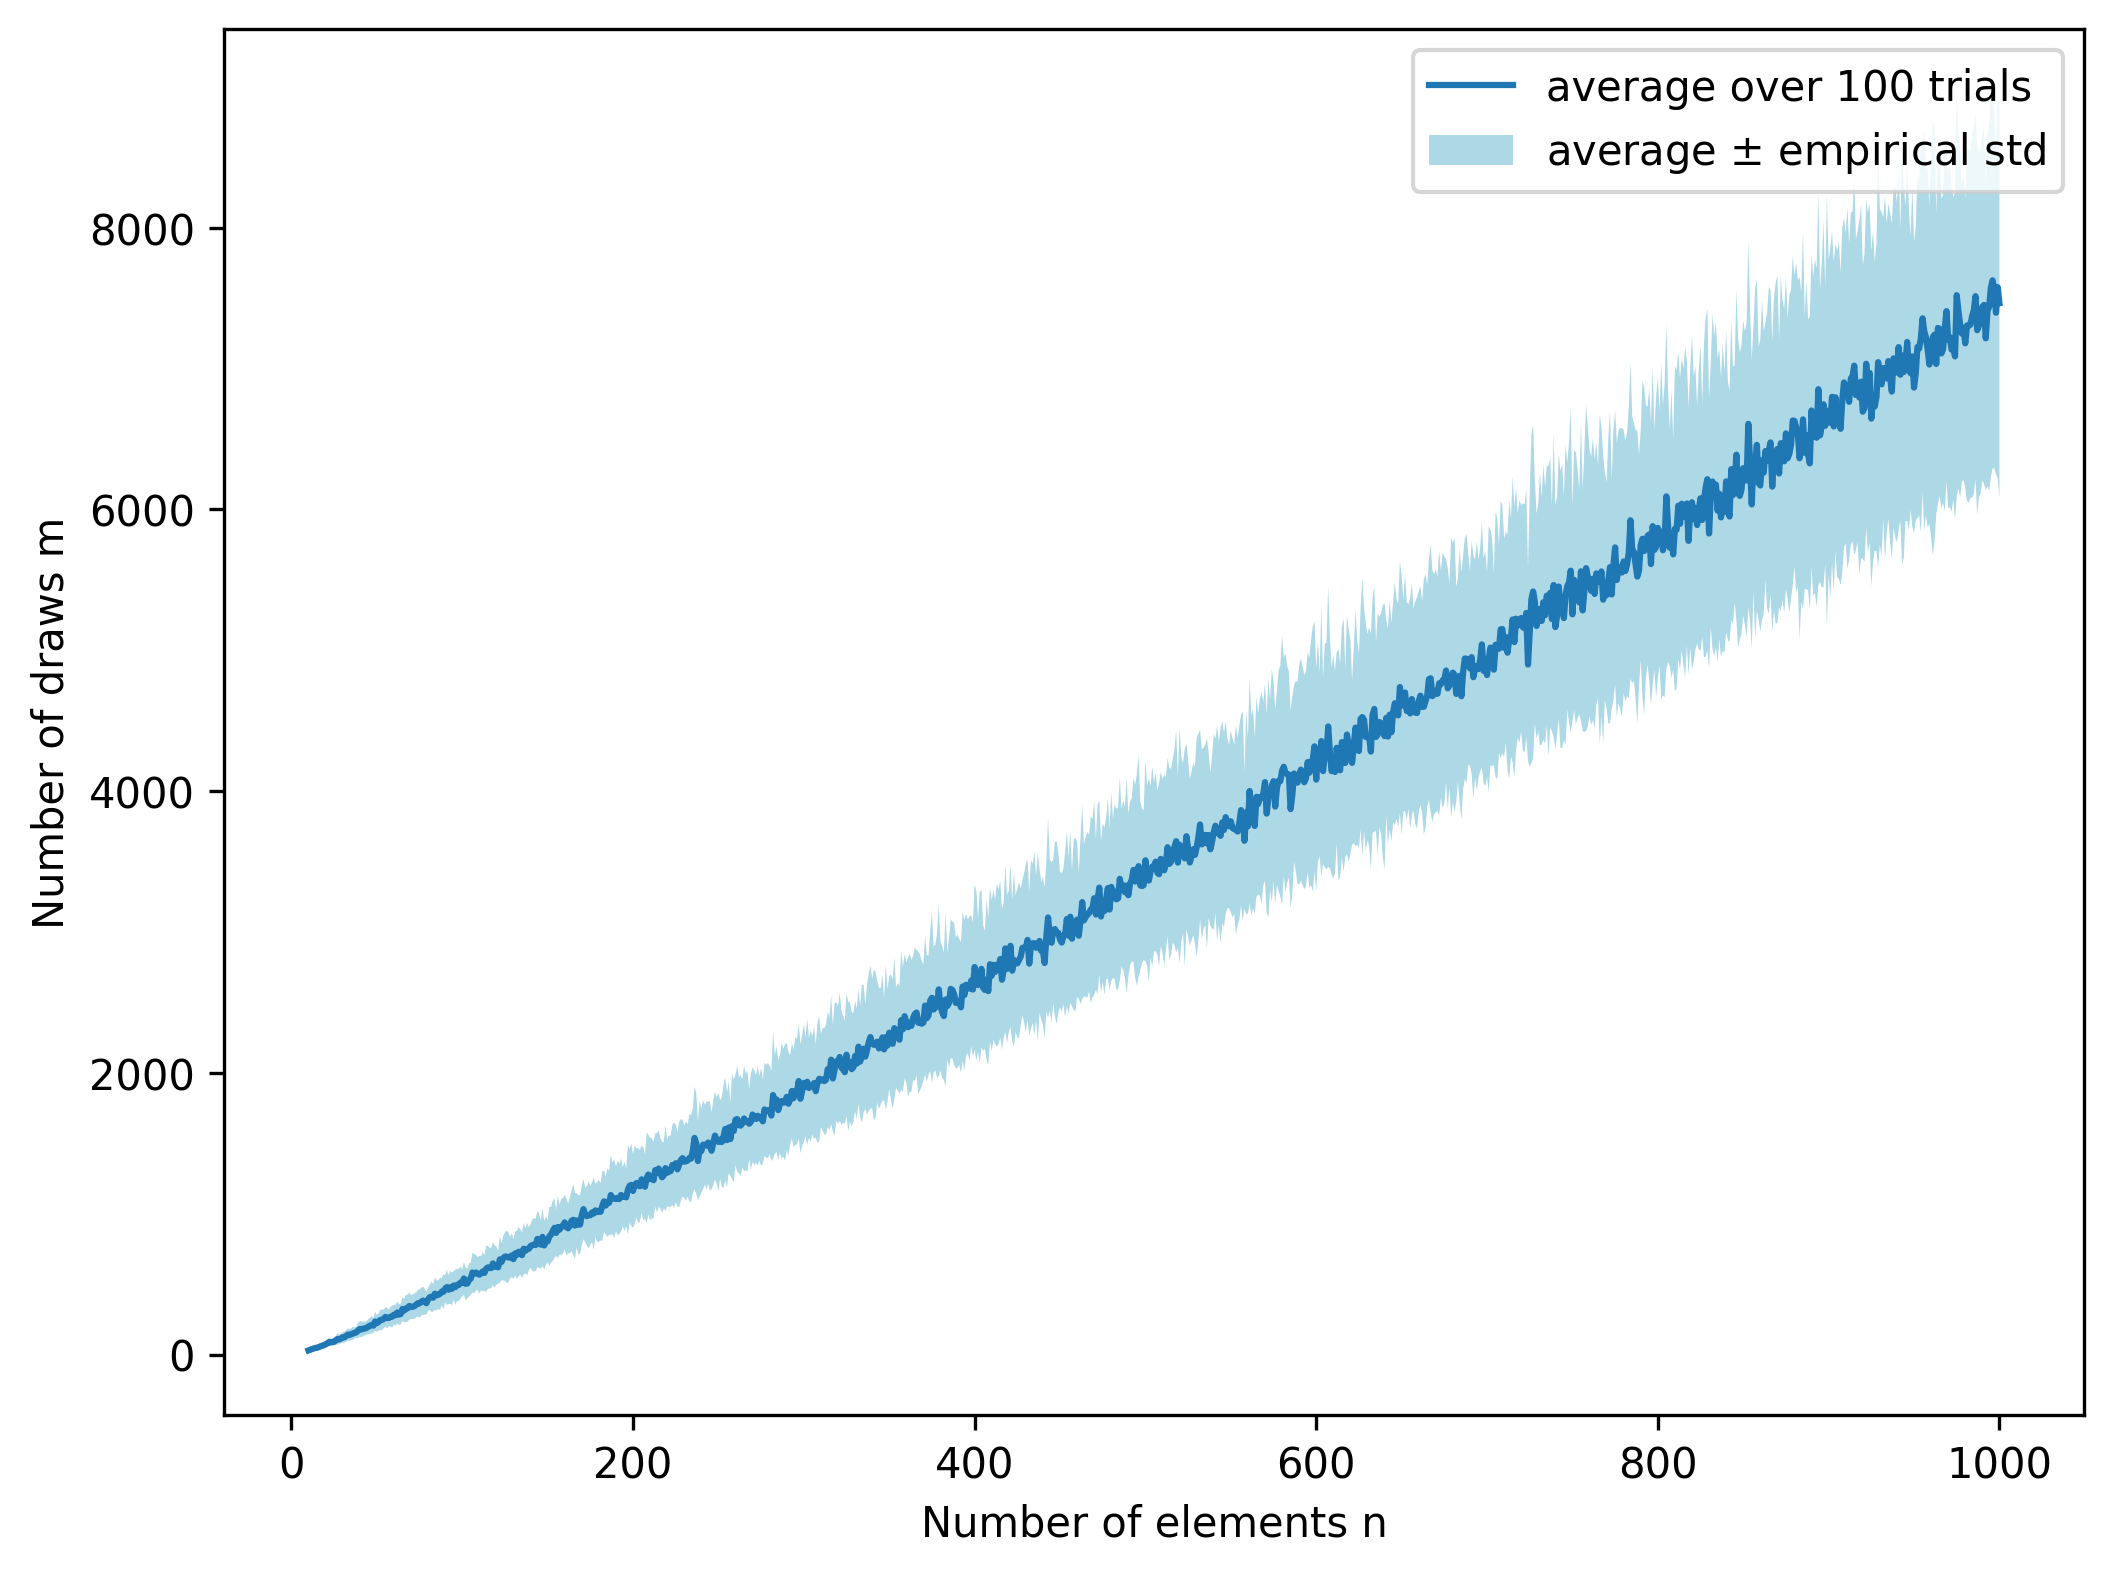
\includegraphics[width=0.9\textwidth]{figures/fig-coverage1.png}
\caption{Average (over 100 trials) of the number of balls thrown until all of the $\nbins$ bins contain at least one ball, as a function of $\nbins$. The range given by one empirical standard deviation is plotted alongside.}
\end{figure}

Looking at the graph above, we can see how the average number of balls to throw grows with $\nbins$. But what is it, quantitatively? How does $\green{M}(\nbins)$ behaves?
\begin{itemize}
    \item $\Theta(\nbins)$?
    \item $\Theta(\nbins\log\nbins)$?
    \item $\Theta(\nbins^{3/2})$?
    \item Something else?
\end{itemize}
And \emph{why}?

\paragraph{Some intuition.} Let's look at what happens when $\nballs=\nbins$: how many bins \emph{haven't} been hit by a balls when we have thrown $\nbins$ of them. The probability a fixed bin does not contain any ball is
\[
\Paren{1-\frac{1}{\nbins}}^{\nbins} \approx e^{-1}
\]
and so the expected number of bins with no balls, by linearity of expectation, is
\begin{equation}
    \label{eq:expected:empty:bins}
\expect{\text{empty bins after }\nbins\text{  balls}}=\sum_{i=1}^{\nbins} \probaOf{\substack{\text{bin $i$ empty}\\\text{ after }\nbins\text{  balls}}} =\nbins\cdot \Paren{1-\frac{1}{\nbins}}^{\nbins} \approx \frac{\nbins}{e}
\end{equation}
This means that after throwing $\nbins$ balls, we still have a constant fraction ($\approx 1/e$) of bins to still hit. Repeating the argument, if we throw $\nbins$ more balls, we expect to still have $\approx 1/e^2$ empty bins; $\nbins$ more balls, and the remaining fraction will be $\approx1/e^3$; etc. Each time we throw $\nbins$ more balls, we decrease (in expectation) the number of empty bins by a constant factor, so\dots{} to bring the expected number of empty bins to $<1$, we'll need to repeat that $\Theta(\log\nbins)$ times.\marginnote{Generalise~\cref{eq:expected:empty:bins} to $\nballs$ bins, to compute directly \[\expect{\text{empty bins after }\nballs\text{  balls}}\] and solve for $\nballs$ to get this expectation to be less than $1$, say $1/2$. Show you retrieve the $\Theta(\nbins\log\nbins)$.} This argument tells us that 
\[
\green{M}(\nbins) = \Theta(\log\nbins)\cdot \nbins = \Theta(\nbins\log\nbins)
\]
sounds reasonable. Can we prove it?

\begin{theorem}
    \label{theo:coupon:collector:expectation}
    We have 
    \[
    \green{M}(\nbins) = \nbins H_{\nbins}\,.
    \]
    where $H_{\nbins} = \sum_{k=1}^{\nbins} \frac{1}{k}$ is the $\nbins$-th Harmonic number.
\end{theorem}
\noindent Before proving this, recall the following fact:\marginnote{Prove the first-order term: $H_n = \Theta(n\log n)$.} % Tutorial
\begin{fact}
\label{fact:harmonic}
    The $n$-th Harmonic number satisfies
    \[
        H_n = \ln n + \gamma + O(1)\,,
    \]
    where $\ln$ is the natural logarithm and $\gamma\approx 0.5772$ is the Euler--Mascheroni constant.
\end{fact}
\begin{proof}[Proof~of~\cref{theo:coupon:collector:expectation}]
To establish this result, we will introduce some auxiliary random variables, so that we can reduce everything to the one good tool we have~--~linearity of expectation. For $1\leq i\leq \nbins$, denote by $T_i$ the number of balls needed, after hitting the $(i-1)$-th distinct bin so far, to hit a new one (the $i$-th bin). So for instance, $T_1=1$ (the first ball we throw by definition hits a new bin, and we had not hit any before), and $T_2$ is the number of balls we need to throw after that to get a ball in another bin than that first one. It's at least $1$, and, if we're unlucky and keep throwing balls into the very same bin, could be much more than that.

The total number of balls to throw before hitting all bins is then, by definition,
\[
T_1+T_2+\cdots+T_{\nbins}
\]
and so, by linearity of expectation,
\begin{equation}
    \label{expect:coverage:proofstep}
\green{M}(\nbins) = \expect{T_1+T_2+\cdots+T_{\nbins}}
= \sum_{i=1}^{\nbins} \expect{T_i}\,.
\end{equation}
It remains to get a handle on $\expect{T_i}$, for $i\geq 1$. We have seen that $T_1=1$ always, so $\expect{T_1}=1$; what about $i\geq 2$? Given that we have hit $i-1$ distinct bins already, the next ball we throw has a probability
\[
\frac{\nbins-(i-1)}{\nbins} = \frac{\nbins-i+1}{\nbins}
\]
to hit one of the remaining empty $\nbins-(i-1)$ bins, out of $\nbins$ total. We keep throwing balls, each with this probability of success, until we do hit an empty bin: so $T_i$ is a Geometric random variable\marginnote{See previous chapter.} with parameter $p_i \eqdef \frac{\nbins-i+1}{\nbins}$, and so its expectation is
\[
    \expect{T_i} = \frac{1}{p_i} = \frac{\nbins}{\nbins-i+1}\,.
\]
Plugging this in~\eqref{expect:coverage:proofstep} gives us
\[
\green{M}(\nbins) = \sum_{i=1}^{\nbins} \frac{\nbins}{\nbins-i+1}
= \sum_{j=1}^{\nbins} \frac{\nbins}{j}
= \nbins H_{\nbins}
\]
concluding the proof.
\end{proof}
Before going further, let us see how this identity we just proved compared to our empirical average:
\begin{figure}[htbp]\centering
    \label{fig:coverage:2}
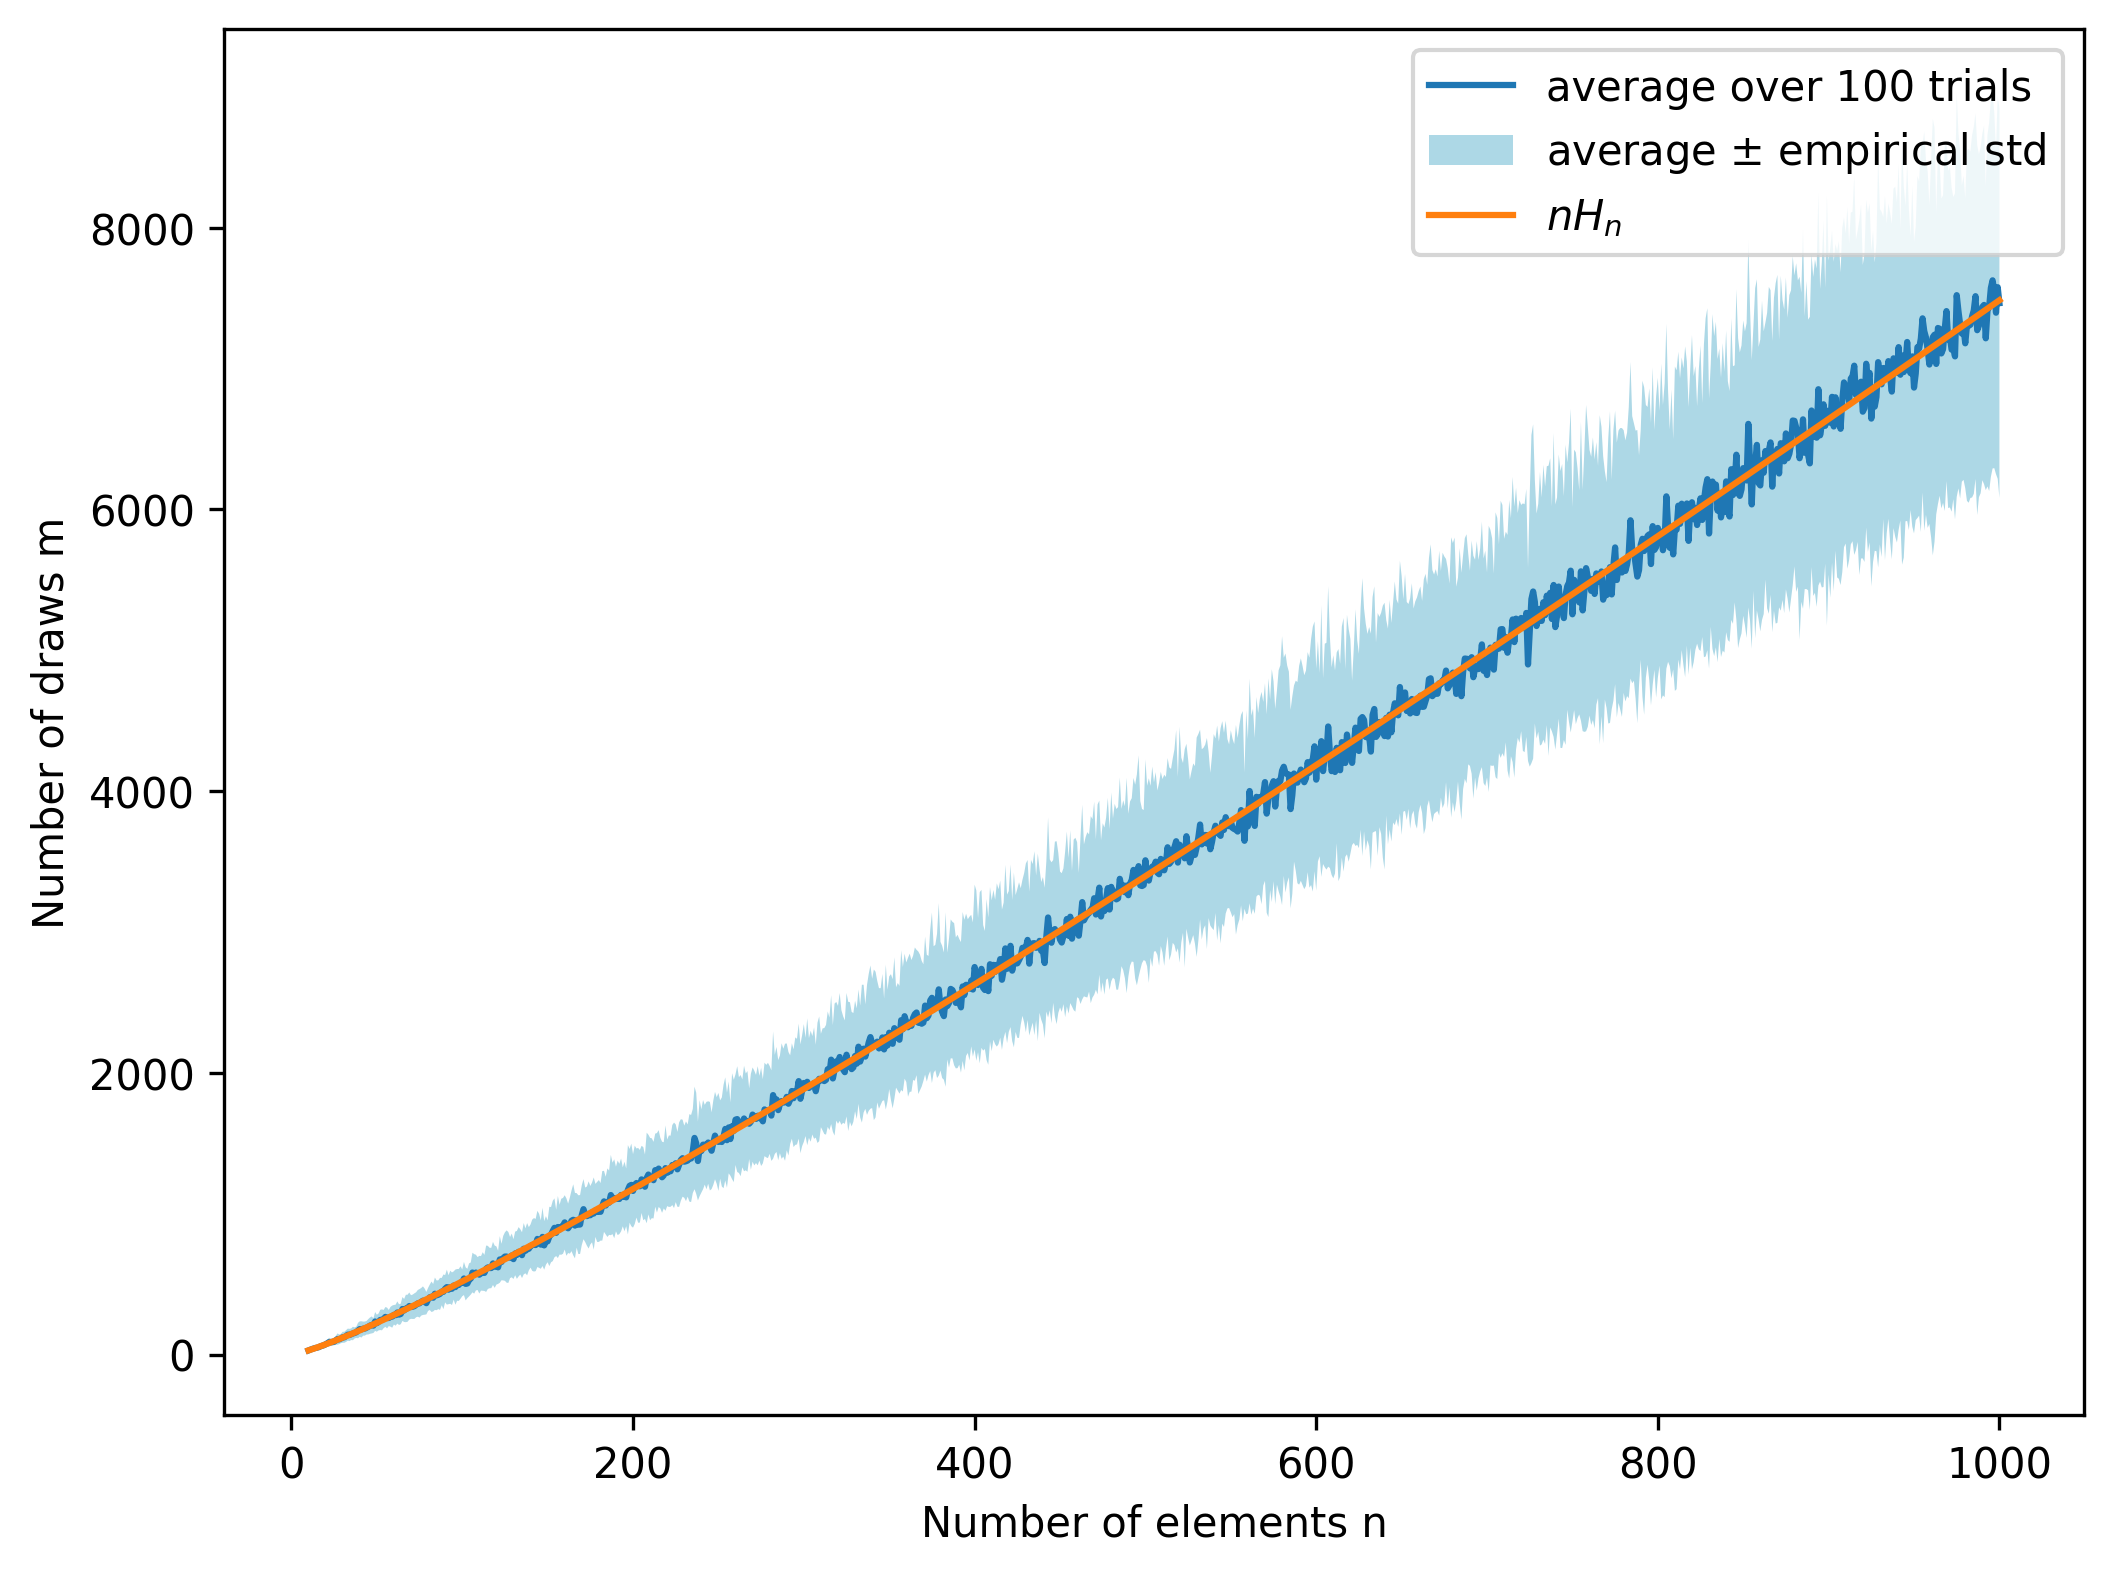
\includegraphics[width=0.9\textwidth]{figures/fig-coverage2.png}
\caption{Average (over 100 trials) of the number of balls thrown until all of the $\nbins$ bins contain at least one ball, as a function of $\nbins$, along with the theoretical value $\nbins H_{\nbins}$ shown in~\cref{theo:coupon:collector:expectation}. The range given by one empirical standard deviation is plotted alongside.}
\end{figure}

Not bad! That does it for the expectation\dots{} but the figure also hints the variance is not too bad, and the number of balls needed to hit all $\nbins$ looks quite concentrated around its expectation. To confirm this (in view of, if we wanted to, applying Chebyshev's inequality), can we also compute the variance?

The amazing thing is that not only we \emph{can}, it's also quite easy.
\begin{theorem}
    \label{theo:coupon:collector:variance}
    The variance of the number $\green{m}(\nbins)$ of bins needed to hit all $\nbins$ bins satisfies
    \[
    \var[\green{m}(\nbins)] \leq \frac{\pi^2}{6}\nbins^2\,.
    \]
\end{theorem}
\begin{proof}
    We start as in the proof of~\cref{theo:coupon:collector:expectation}, writing
    \[
        \green{m}(\nbins) = T_1+\dots+T_{\nbins}
    \]
    The crucial observation is that (suprinsingly?), \emph{the random variables $T_1,\dots,T_{\nbins}$ are independent.} Intuitively, this is because, once you have hit $i-1$ bins, the number of \emph{new} balls you need to cover the remaining $\nbins-(i-1)$ does not depend on how many balls you already threw: it only depends on $\nbins$ and $i$, and ``doesn't care about the past.''\marginnote{This is called the \href{https://en.wikipedia.org/wiki/Geometric_distribution\#General_properties}{memorylessness property} of the geometric distribution, but try to first convince yourself of this without giving it a label.}

    This is great, because computing the variance becomes immediate:
    \[
    \var[\green{m}(\nbins)]=\var[T_1+\dots+T_{\nbins}]
    = \sum_{i=1}^{\nbins} \var[T_i]
    \]
    and we already saw that $T_i \sim \operatorname{Geom}\Paren{p_i}$ with $p_i=\frac{\nbins-i+1}{\nbins}$, ``so'' its variance is \marginnote{Check it yourself: we don't lose much by ignoring the $-p_i$ term.}
    \[
    \var[T_i] = \frac{1-p_i}{p_i^2} \leq \frac{1}{p_i^2}= \frac{\nbins^2}{(\nbins-i+1)^2}
    \]
    and we get
    \[
    \var[\green{m}(\nbins)]
    \leq \nbins^2\cdot\sum_{i=1}^{\nbins} \frac{1}{(\nbins-i+1)^2}
    =\nbins^2\cdot\sum_{j=1}^{\nbins} \frac{1}{j^2}
    \leq \nbins^2\cdot \frac{\pi^2}{6}\,,
    \]
    the last inequality recalling that
    $\sum_{k=1}^{\infty}\frac{1}{k^2} = \frac{\pi^2}{6}$.
\end{proof}
We won't go through too much here, but for instance, by Chebyshev's inequality, this means that
\begin{equation}
    \green{m}(\nbins) = \nbins H_{\nbins} \pm O(\nbins)
\end{equation}
with probability at least $0.99$; combining this with~\cref{fact:harmonic}, similarly,
\begin{equation}
    \green{m}(\nbins) = \nbins \ln \nbins \pm O(\nbins)
\end{equation}
with probability at least $0.99$ (with a different constant in the $O(\cdot)$).

To conclude this part\dots{} how did we do with this variance bound? Well, let us see the empirical simulation again, adding them to the mix:
\begin{figure}[htbp]\centering
    \label{fig:coverage:3}
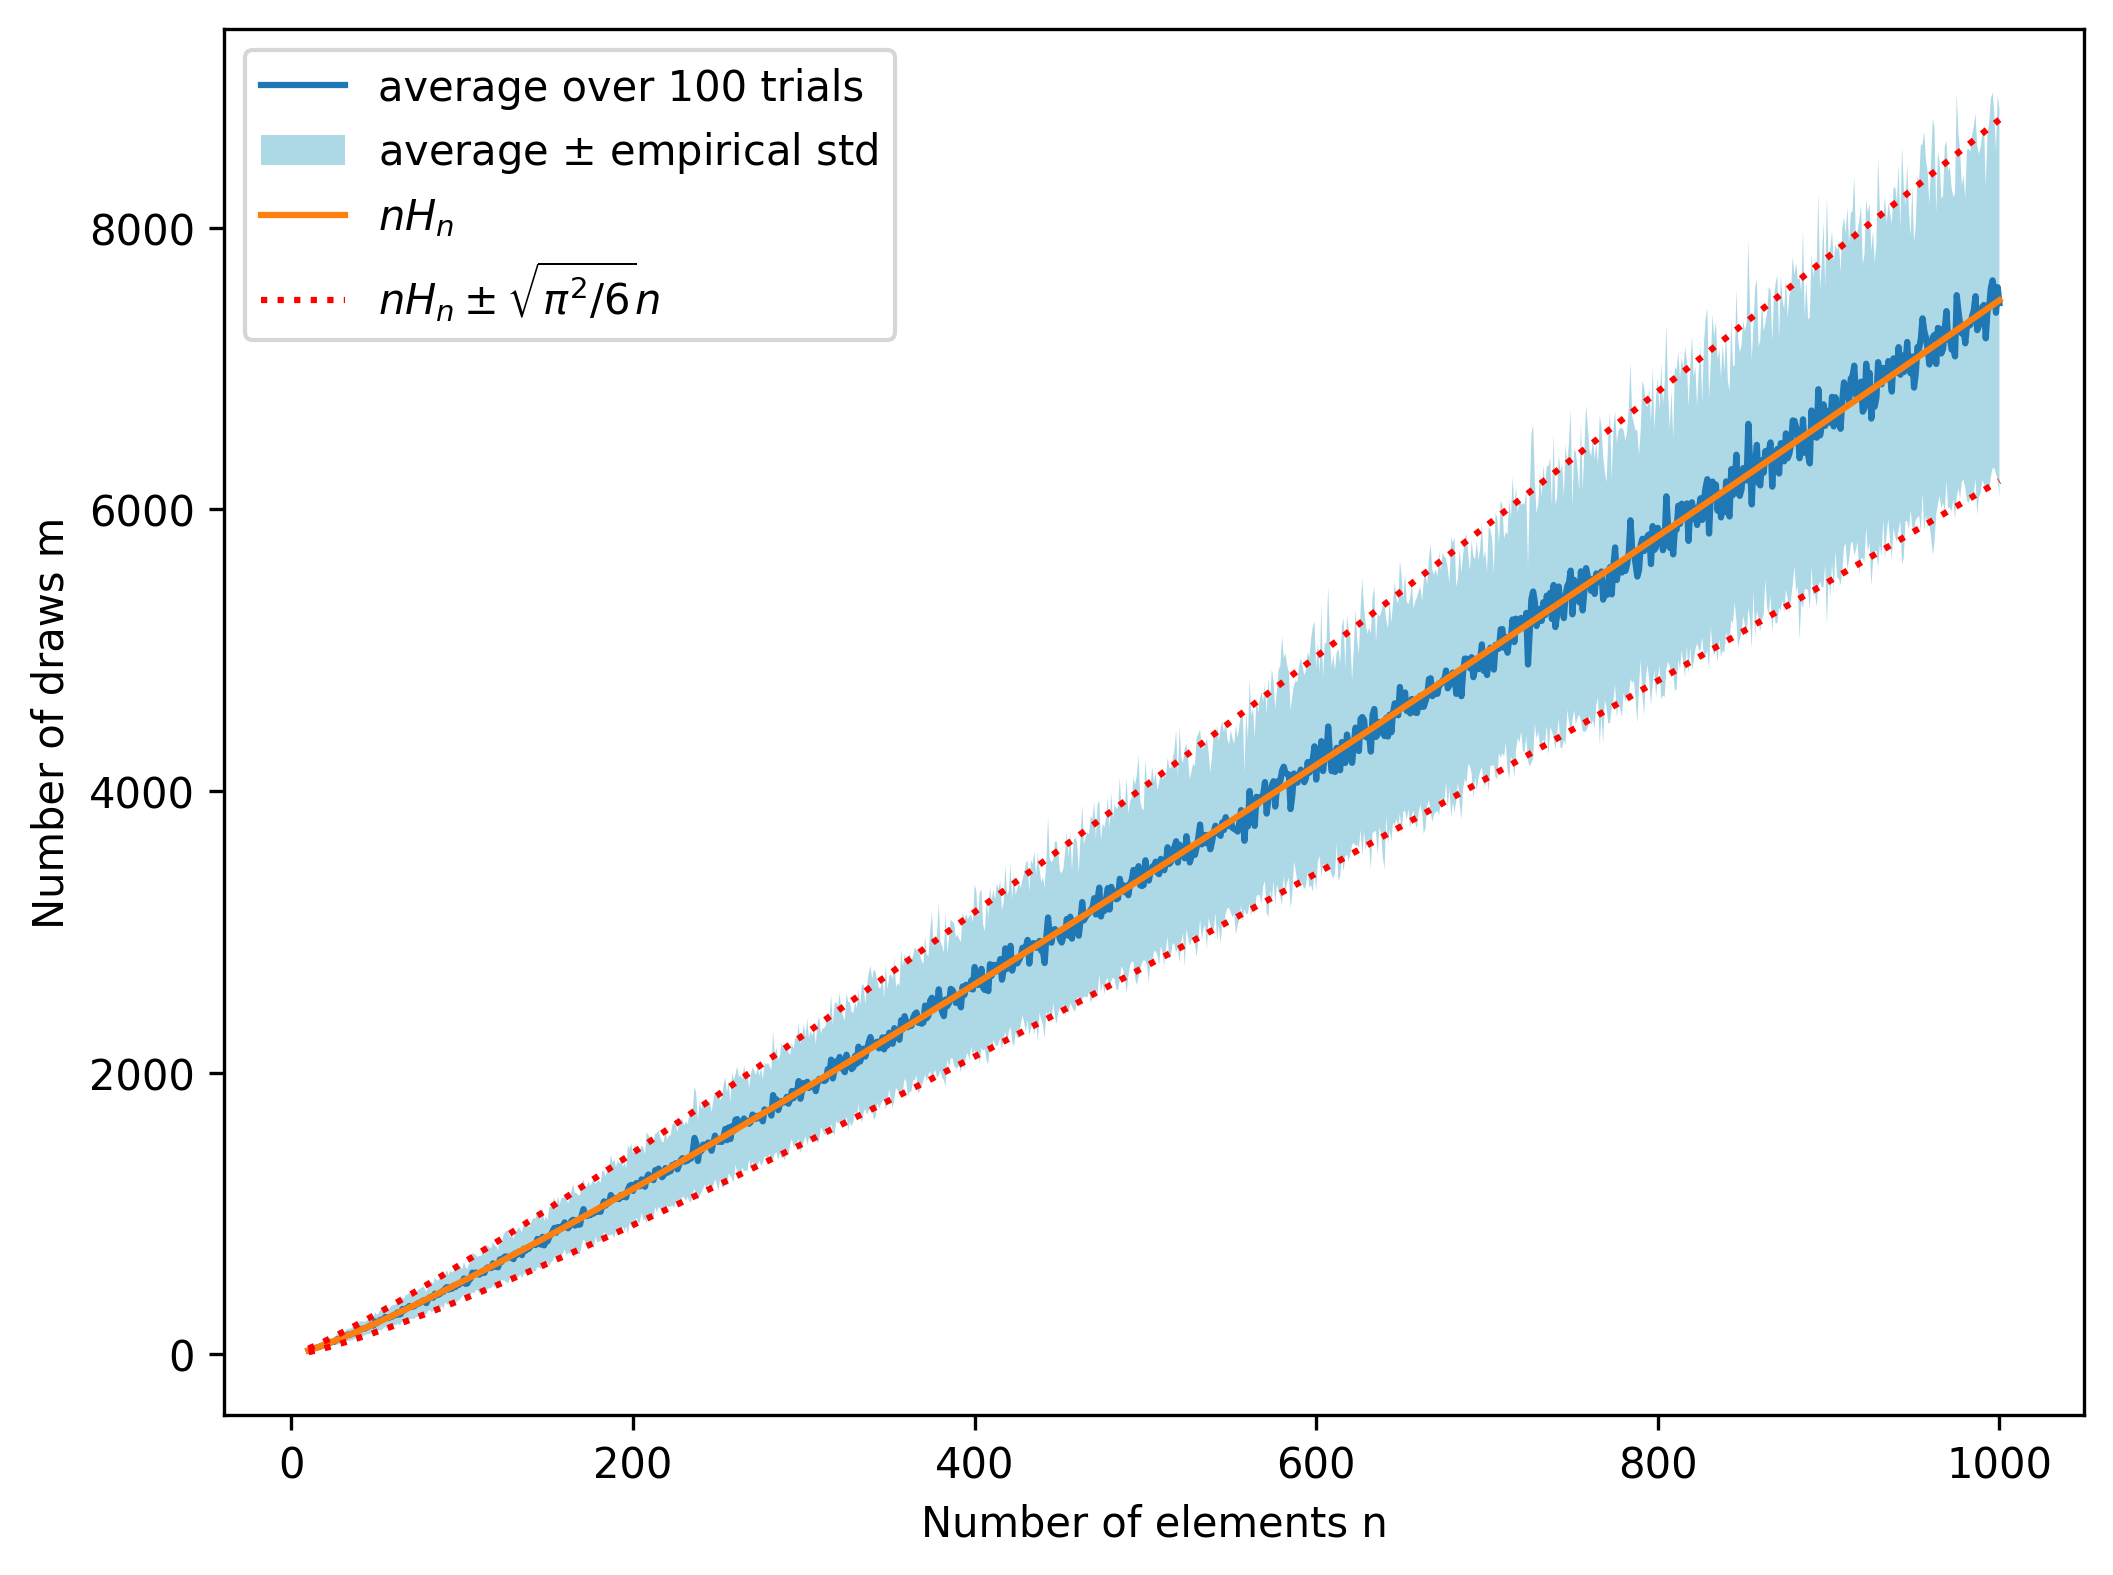
\includegraphics[width=0.9\textwidth]{figures/fig-coverage4.png}
\caption{Average (over 100 trials) of the number of balls thrown until all of the $\nbins$ bins contain at least one ball, as a function of $\nbins$, along with the theoretical value $\nbins H_{\nbins}$ shown in~\cref{theo:coupon:collector:expectation}. The range given by one empirical standard deviation is plotted alongside, as well as the theoretical standard deviation bound obtained.}
\end{figure}

Quite good!

% fun? https://math.stackexchange.com/questions/4051815/intuition-behind-the-coupon-collector-problem-is-there-inclusion-exclusion-prin

\section{Load balancing}
For the last problem considered in this chapter, let us fix $\nballs = \nbins$, and look at how ``balanced'' the bin contents are. In particular, we will be interested in the \emph{maximum load} of the bins:\marginnote{This has applications to, \eg resource allocations, scheduling, etc.}
\begin{framed}
We throw $\nbins$ balls into $\nbins$ bins: what the (expected) number $\orange{L}(\nbins)$ of balls the \emph{fullest} bin will contain?
\end{framed}
Let us denote by $\orange{L}_1,\dots,\orange{L}_{\nbins}$ the number of balls contained in each of the $\nbins$ bins. We have, of course, $\orange{L}_i \leq \nbins$ (number of balls in total) for every $i$. But that's\dots{} quite weak.

It is not hard to see that each bin, separately, follows a Binomial distribution with parameters $\nbins$ and $1/\nbins$\marginnote{Each $\orange{L}_i$ is a $\binomial{\nbins}{1/\nbins}$ random variable: but $\orange{L}_1,\dots,\orange{L}_{\nbins}$ are \emph{not} independent.} and so bin $i$ will have expected load 
\[
\expect{\orange{L}_i} = \nbins\cdot \frac{1}{\nbins} = 1
\]and we also get 
\[
\var[\orange{L}_i] = \nbins\cdot \frac{1}{\nbins}\Paren{1-\frac{1}{\nbins}} \leq 1
\]
This implies, By Chebyshev's inequality, that for each $1\leq i\leq \nbins$, and setting $t \eqdef \sqrt{2\nbins}$,
\[
\probaOf{ \orange{L}_i \geq 1+\sqrt{2\nbins} } \leq \probaOf{ |\orange{L}_i - \expect{\orange{L}_i}| \geq t } \leq \frac{\var[\orange{L}_i]}{t^2} \leq \frac{1}{2\nbins}
\]
and so, by a union bound over the $\nbins$ bins, 
\[
\probaOf{ \max_{1\leq i\leq\nbins}\orange{L}_i \geq 1+\sqrt{2\nbins} } \leq \nbins\cdot \frac{1}{2\nbins} =  \frac{1}{2}
\]
That ``simple'' application of Chebyshev shows the maximum load $\orange{L} = \max_{1\leq i\leq\nbins}$ is $O(\sqrt{\nbins})$ with constant probability. But is it tight? And what does that tell us about $\orange{L}(\nbins)=\expect{\orange{L}}$?\medskip

As in the previous sections, before jumping to conclusions, let's run a simulation.
\begin{lstlisting}
def maxload(n,m):
    loads = np.zeros(n, dtype=int)
    for _ in range(m):
        draw = random.randint(1, n);
        loads[draw-1] += 1
    return np.max(loads)
\end{lstlisting}
\begin{lstlisting}
list_n = np.arange(10, 1001);
experiments_maxload_avg = np.zeros(np.size(list_n));
experiments_maxload_std = np.zeros(np.size(list_n));
for i in range(len(list_n)):
    maxload_trials = [maxload(list_n[i],list_n[i]) for _ in range(100)];
    experiments_maxload_avg[i] = np.mean(maxload_trials);
    experiments_maxload_std[i] = np.std(maxload_trials);
\end{lstlisting}
\begin{figure}[htbp]\centering
    \label{fig:maxload:1}
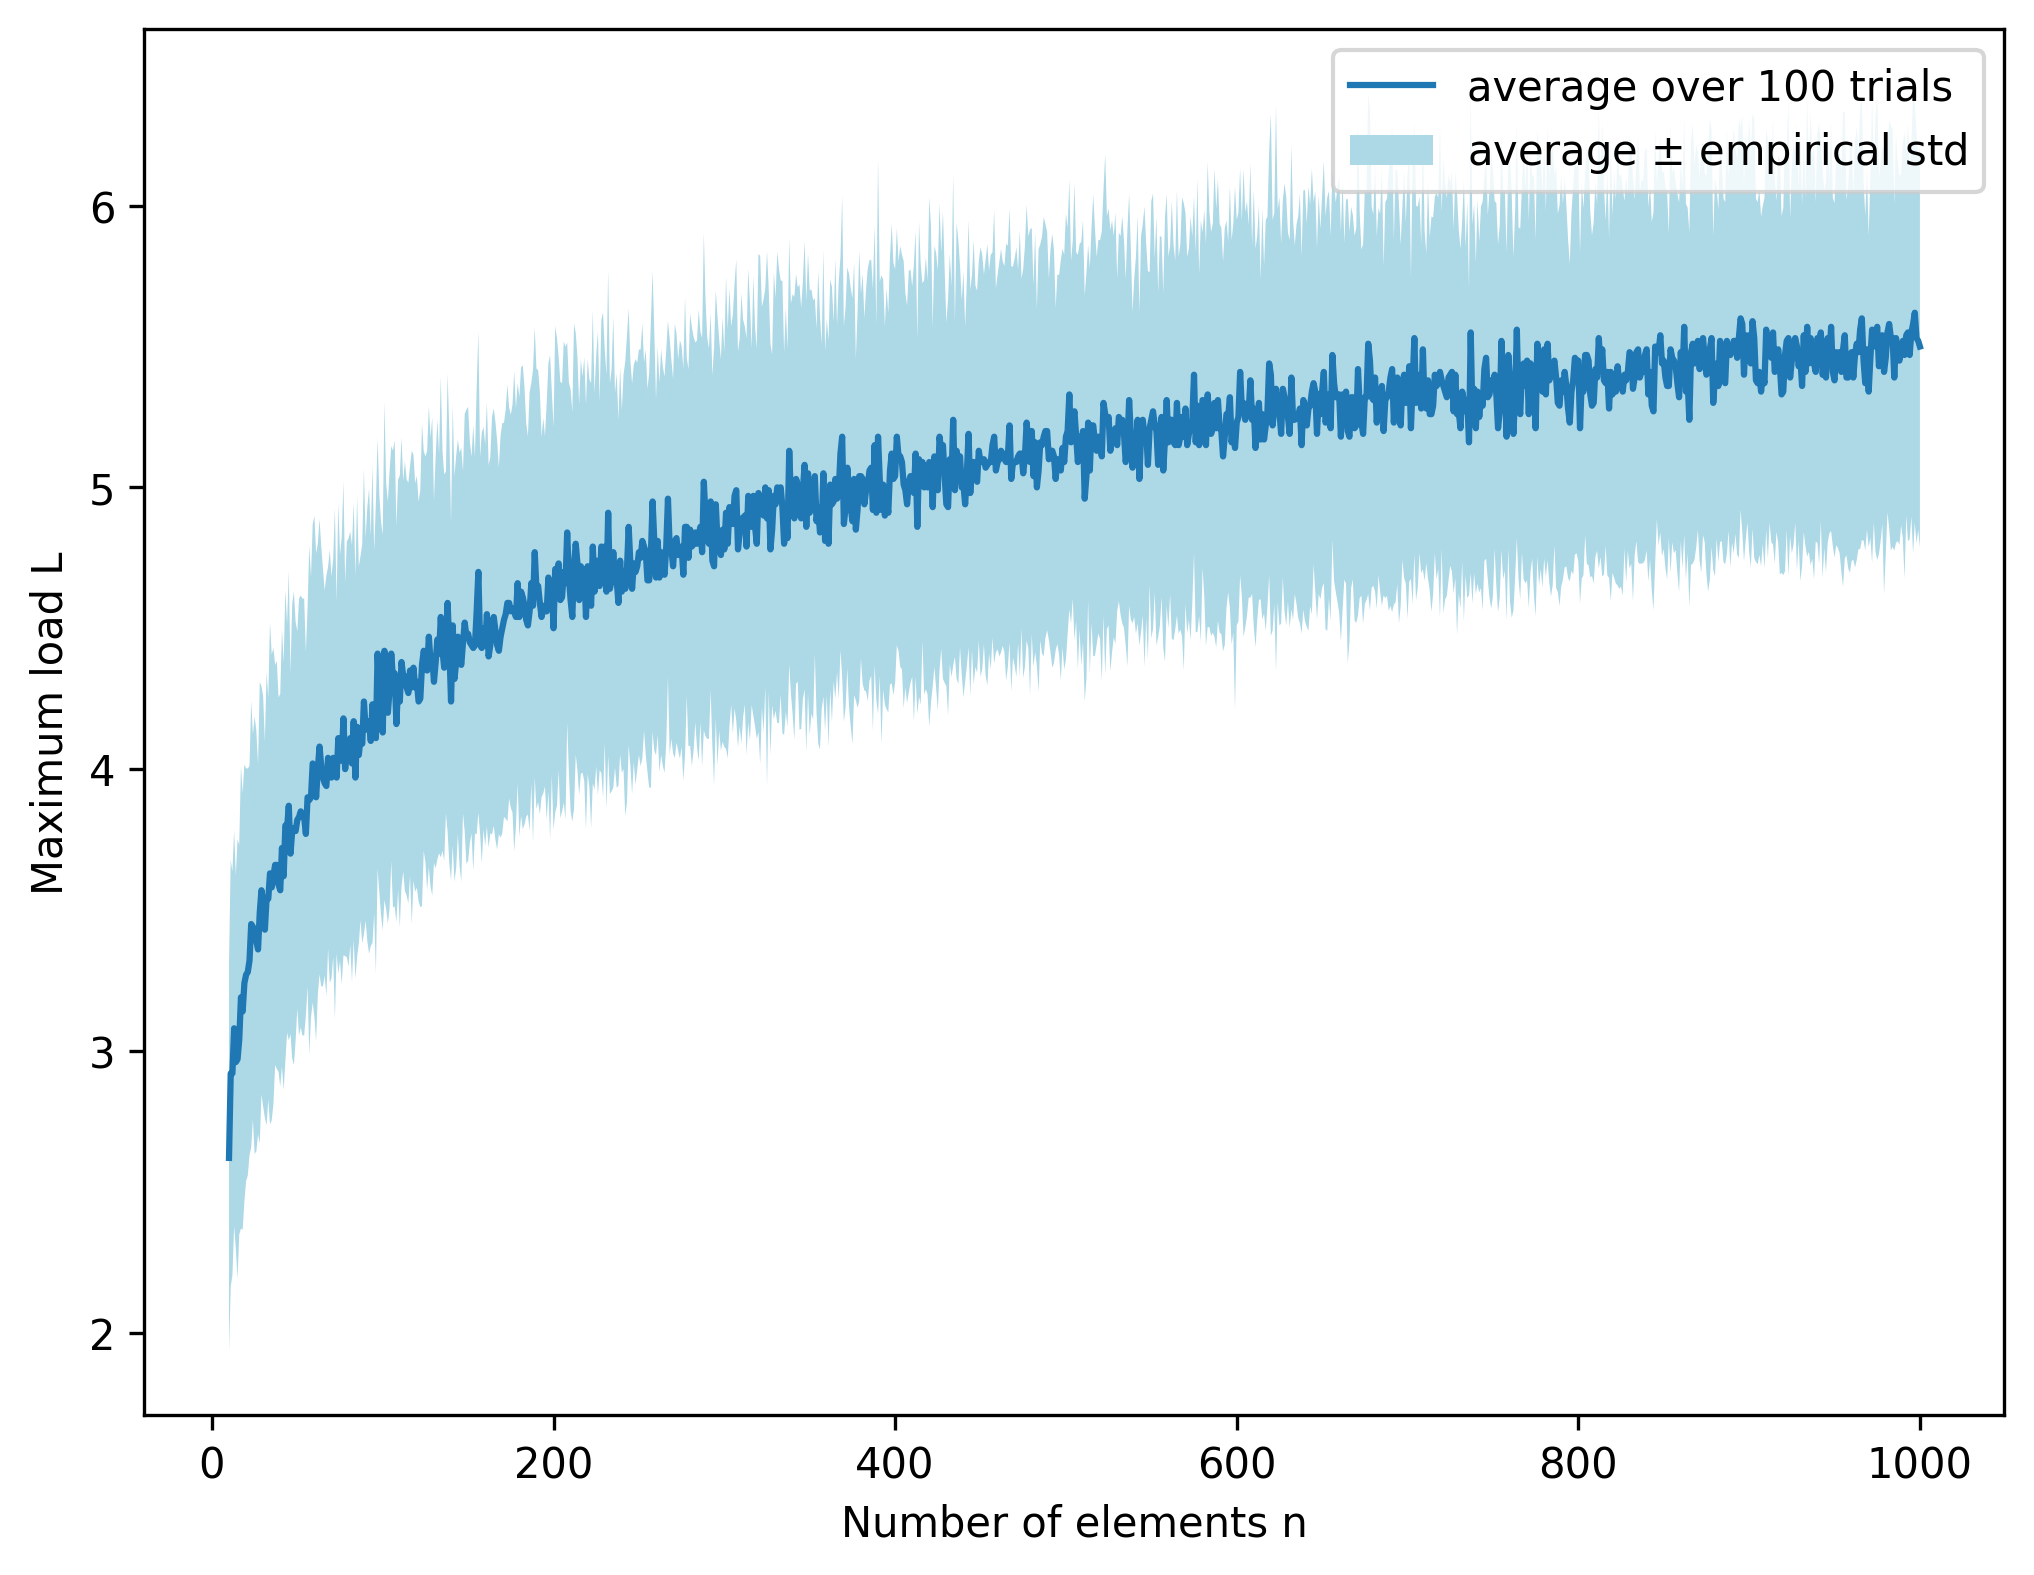
\includegraphics[width=0.9\textwidth]{figures/fig-maxload1.png}
\caption{Average (over 100 trials) of the maximum load when throwing $\nbins$ balls into $\nbins$ bins, as a function of $\nbins$. The range given by one empirical standard deviation is plotted alongside.}
\end{figure}

Looking at the graph (\cref{fig:maxload:1}), we can see how the average maximum load grows with $\nbins$. But what is it, quantitatively? How does $\orange{L}(\nbins)$ behaves?
\begin{itemize}
    \item $\Theta(\log\nbins)$?
    \item $\Theta(\sqrt{\nbins})$?
    \item $\Theta(\nbins)$?
    \item Something else?
\end{itemize}
And \emph{why}?\marginnote{This one will be tough.}\medskip

We will show that, oddly, the answer is ``something else.'' Something quite surprising:
\begin{theorem}
    \label{theo:maxload}
    The expected maximum load $\orange{L}(\nbins)$ when throwing uniformly and independently $\nbins$ balls into $\nbins$ bins grows as
    \[
        \orange{L}(\nbins) = \bigTheta{\frac{\log\nbins}{\log\log\nbins}}\,.
    \]
\end{theorem}
\begin{proof}[Proof of the upper bound of~\cref{theo:maxload}]
Fix any $1\leq i\leq \nbins$, and consider the load in bin $i$. For $0\leq \ell\leq \nbins$, we will give an upper bound on the probability that at least $\ell$ balls fall in this bin: namely, 
\begin{equation}
    \probaOf{\orange{L}_i \geq \ell} 
    \leq \frac{1}{\ell^\ell} 
\end{equation}
To prove this: $\probaOf{\orange{L}_i \geq \ell}$ is the probability that there exists a subset $S\subseteq[\nbins]$ of size at least $\ell$ (a subset of our $\nbins$ balls), and these $|S|$ balls are \emph{exactly} the ones which fell in the $i$-th bin (not a single other): for a fixed $S$, this has probability $\Paren{\frac{1}{\nbins}}^{|S|}\Paren{1-\frac{1}{\nbins}}^{\nbins-|S|}$. We \emph{could} write exactly
\begin{align*}
    \probaOf{\orange{L}_i \geq \ell} 
    &=
    \sum_{\substack{S\subseteq [\nbins]\\ |S| \geq \ell}} \frac{1}{\nbins^{|S|}}\Paren{1-\frac{1}{\nbins}}^{\nbins-|S|} 
    = \sum_{k=\ell}^{\nbins} \sum_{\substack{S\subseteq [\nbins]\\ |S| = k}} \frac{1}{\nbins^{k}}\Paren{1-\frac{1}{\nbins}}^{\nbins-k} \\
    &= \sum_{k=\ell}^{\nbins} \binom{\nbins}{k}\frac{1}{\nbins^{k}}\Paren{1-\frac{1}{\nbins}}^{\nbins-k} %\tag{$\binom{\nbins}{k}$: number of subsets of size $k$}\\
%    &\leq \binom{\nbins}{\ell}\frac{1}{\nbins^{\ell}}\Paren{1-\frac{1}{\nbins}}^{\nbins-\ell}\\
%    &\leq \binom{\nbins}{\ell}\frac{1}{\nbins^{\ell}} 
\end{align*}
the last line recalling that $\binom{\nbins}{k}$ is number of subsets of $[\ns]$ of size $k$, and try to bound that last expression: it is possible, but rather annoying (as binomial coefficients often are), and we do not need to be \emph{that} precise: we just need a good enough upper bound! So we can instead allow ourselves a bit of double-counting: let us simply sum over all subsets $S$ of size \emph{exactly} $\ell$, and focus on the probability that all these $\ell$ balls fall in bin $i$. The other $\ns-\ell$ balls could fall anywhere, including in bin $i$:\footnote{That's the ``we may be double-counting some events'' part.} we don't really care, as long as the upper bound we end up with is not too loose.\marginnote{Exercise: check that $\sum_{k=\ell}^{\nbins} \binom{\nbins}{k}\frac{1}{\nbins^{k}}\Paren{1-\frac{1}{\nbins}}^{\nbins-k} \leq \binom{\nbins}{\ell}\frac{1}{\nbins^{\ell}}$ via a direct computation.}
\begin{align*}
    \probaOf{\orange{L}_i \geq \ell} 
    &\leq
    \sum_{\substack{S\subseteq [\nbins]\\ |S| = \ell}} \probaOf{\text{all }\ell \text{ balls indexed by } S \text{ fall in bin } i} \\
    &=  \sum_{\substack{S\subseteq [\nbins]\\ |S| = \ell}} \left(\frac{1}{\ns}\right)^\ell \\
    &= \binom{\nbins}{\ell}\frac{1}{\nbins^{\ell}} \tag{There are $\binom{\ns}{\ell}$ subsets of size $\ell$}
\end{align*}
From here, we will use this \emph{very} convenient and useful inequality on binomial coefficients:\marginnote{Another life saver.}
\begin{fact}
    \label{fact:binom:coeffs}
    For every $1\leq k\leq n$,
    \[
        \Paren{\frac{n}{k}}^k 
        \leq \binom{n}{k} 
        \leq \Paren{\frac{e n}{k}}^k\,.
    \]
\end{fact}
\noindent This directly leads to the claimed bound
\[
    \probaOf{\orange{L}_i \geq \ell} 
    \leq \Paren{\frac{e \nbins}{\ell}}^{\ell}\frac{1}{\nbins^{\ell}} 
    = \frac{e^\ell}{\ell^\ell}\,.
\]
By a union bound over all $1\leq i\leq \nbins$, we can then conclude that, for every $\ell \geq 1$,
\begin{equation}
    \probaOf{\orange{L} \geq \ell} \leq \sum_{i=1}^{\nbins}\probaOf{\orange{L}_i \geq \ell}
    \leq \frac{\nbins e^\ell}{\ell^\ell}
\end{equation}
This is a very good bound for large $\ell$, but it is quite useless for small $\ell$: for instance, for $\ell=1$, it gives a vacuous bound! Of course, another bound we have is $\probaOf{\orange{L} \geq \ell}  \leq 1$. We will need that, too. Let $\ell(\nbins)$ be the smallest value such that\marginnote{This is the value of $\ell$ starting at which we should switch from using $\probaOf{\orange{L} \geq \ell}  \leq 1$ to using $\probaOf{\orange{L} \geq \ell}  \leq \frac{\nbins e^{\ell}}{\ell^\ell}$, as the latter becomes better.}
\begin{equation}
    \ell(\nbins)^{\ell(\nbins)}e^{-\ell(\ns)} \geq \nbins\,.
\end{equation}
Alright: let us proceed to bounding the expectation of $\orange{L}$. We can write, since $\orange{L}$ is a non-negative integer-valued random variable,\marginnote{Dividing the summation in two parts and using a different bound for both is a standard, handy trick.}
\begin{align}
    L(\nbins) = \expect{\orange{L}} 
    &= \sum_{\ell=1}^\infty \probaOf{\orange{L} \geq \ell} \notag\\
    &= \sum_{\ell=1}^{\ell(\nbins)} \probaOf{\orange{L} \geq \ell} + \sum_{\ell=\ell(\nbins)+1}^\infty \probaOf{\orange{L} \geq \ell} \notag\\
    &\leq \sum_{\ell=1}^{\ell(\nbins)} 1 + \sum_{\ell=\ell(\nbins)+1}^\infty \frac{\nbins e^\ell}{\ell^\ell} \tag{Where the action happens} \notag\\
    &\leq \ell(\nbins) + \sum_{\ell=\ell(\nbins)+1}^\infty \frac{\nbins e^\ell}{\ell(\nbins)^\ell} \notag\\
    &= \ell(\nbins) + \frac{\nbins e^{\ell(\nbins)}}{\ell(\nbins)^{\ell(\nbins)}}\sum_{\ell=\ell(\nbins)+1}^\infty \frac{e^{\ell-\ell(\nbins)}}{\ell(\nbins)^{\ell-\ell(\nbins)}} \notag\\
    &= \ell(\nbins) + \frac{\nbins e^{\ell(\nbins)}}{\ell(\nbins)^{\ell(\nbins)}}\sum_{j=1}^\infty \frac{e^j}{\ell(\nbins)^{j}} \notag\\
    &\leq \ell(\nbins) + \sum_{j=1}^\infty \frac{1}{2^{j}} \tag{as $\frac{\nbins e^{\ell(\nbins)}}{\ell(\nbins)^{\ell(\nbins)}} \leq 1$, and $\ell(\nbins)\geq 2e$} \notag\\
    &= \ell(\nbins) + 1 \label{eq:ub:maxload}
\end{align}
so all that remains to do to conclude is to give an upper bound on $\ell(\nbins)$ itself. This part is not too bad: by definition of $\ell(\nbins)$, we know that
\[
    (\ell(\nbins)-1)^{\ell(\nbins)-1}e^{-(\ell(\nbins)-1))} < \nbins
\]
and taking logarithms, we get
$
(\ell(\nbins)-1)\log (e^{-1}(\ell(\nbins)-1)) < \log \nbins
$. One can ``easily''\marginnote{Exercise: show it.} show that this implies
\[
\ell(\nbins) = \bigTheta{\frac{\log\nbins}{\log\log\nbins}}
\]
which combined with~\eqref{eq:ub:maxload} proves that
$
\boxed{L(\nbins) = \bigO{\frac{\log\nbins}{\log\log\nbins}}}
$.

\paragraph{What about the lower bound?} We will only \emph{sketch} the lower bound in these notes, trying to focus on the key insights. The first insight is that $\orange{L}_1, \dots, \orange{L}_{\nbins}$, which are Binomial r.v.'s with parameters $\nbins$ and $1/\nbins$, are well approximated by a different, ``nicer'' type of of random variable, \emph{Poisson} random variables with parameter $\nbins\cdot 1/\nbins=1$. \marginnote{More generally, 
\[
\boxed{\binomial{n}{\frac{\lambda}{n}} \approx \poisson{\lambda}}
\]
for constant $\lambda>0$. This is very handy!} So we will ``assume'' for convenience\marginnote{This is not an actual proof! But it can be turned into one.} that we can instead consider $\orange{L}'_1, \dots, \orange{L}'_{\nbins} \sim \poisson{1}$. What's more, we will even make the (also not justified! But good for intuition) that these $\orange{L}'_1, \dots, \orange{L}'_{\nbins}$ are independent.

We then can write, since $\expect{\orange{L}} = \sum_{k=1}^\infty \probaOf{\orange{L} \geq k}$, that, for any fixed $\ell\geq 1$ of our choosing,
\begin{align*}
\expect{\orange{L}} &\geq \sum_{k=1}^\ell \probaOf{\orange{L} \geq k} \geq \ell \probaOf{\orange{L} \geq \ell} = 
\ell \probaOf{\exists i,\, \orange{L}_i \geq \ell}
\\
&\approx \ell \probaOf{\exists i,\, \orange{L}'_i \geq \ell}
\geq  \ell \probaOf{\exists i,\, \orange{L}'_i = \ell}
\end{align*}
where the $\approx$ is the first ``sketchy'' Poisson approximation. Using our (unwarranted, sketchy) independence of the $\orange{L}'_i$'s, we can continue by writing\marginnote{If $N\sim\poisson{\lambda}$, then for every non-negative integer $k$
\[
\boxed{\probaOf{N=k} = e^{-\lambda}\frac{\lambda^k}{k!}\,.}
\]}
\begin{align*}
\probaOf{\exists i,\, \orange{L}'_i = \ell}
&= 1-\probaOf{\forall i,\, \orange{L}'_i \neq \ell} \\
&= 1-\Paren{ 1- \frac{e^{-1}}{\ell!} }^{\nbins} \tag{Independence}\\
&\geq 1-e^{-\frac{\nbins}{\ell!}} \tag{using $\ln(1-x)\geq -x$}\\
&\geq 1-e^{-\frac{\nbins}{\ell^\ell}} \tag{using $\ell! \leq \ell^\ell$}\\
\end{align*}
Suitably choosing \[
\ell = \bigTheta{\frac{\log\nbins}{\log\log\nbins}}
\] we get $e^{-\frac{\nbins}{\ell^\ell}} \leq 1/2$, from which $\probaOf{\exists i,\, \orange{L}'_i = \ell} \geq 1/2$. So overall (again, modulo the sketchy bits~--~this is not a full proof), we get
\[
\expect{\orange{L}} \geq \ell \cdot \frac{1}{2} = \bigOmega{\frac{\log\nbins}{\log\log\nbins}}
\]
``showing'' the lower bound.
\end{proof}

\paragraph{Alternative (advanced) proof of the upper bound \advancedstuff} Here is a ``slick'' proof, which seems somewhat magical, but has a couple neat tricks that you will see again or are worth internalizing.\marginnote{Go over it during the tutorials!}

Recall that we want to bound the quantity
\[
\orange{L}(\nbins) = \expect{\max_{1\leq i\leq \nbins} \orange{L}_i}
\]
where the loads $L_1,\dots,L_{\nbins}$ are \emph{not} independent, but all follow a $\operatorname{Binom}(\nbins, 1/\nbins)$ distribution. One can then give an upper bound on $\orange{L}(\nbins)$ as follows.\marginnote{The idea is to replace the $\max$ by a $\sum$ in order to use linearity of expectation~--~but $\max_i \leq \sum_i$ is too lossy, so first we ``exponentiate'' the random variables to mitigate that loss,  as $\max_i \exp \leq \sum_i \exp$ should be ``exponentially less lossy.'' \emph{But} to exponentiate we write $X = \ln \exp X$, which means we now have a $\log$ inside the expectation, and that is not easy to handle: thankfully, $\ln$ is concave, so we can use Jensen's inequality to write $\expect{\ln} \leq \ln\expect{}$. We might also lose something in this step, but that ``Jensen gap'' is typically small for nice, well-concentrated random variables, so\dots{} we can try and hope for the best.}
First, introduce a free parameter $\blue{t}>0$ to be determined later, when we want to optimise the final bound we get.
\begin{align}
    \orange{L}(\nbins) &= \frac{1}{\blue{t}}\cdot \expect{\max_{1\leq i\leq \nbins} \blue{t}\orange{L}_i} \notag\\
    &= \frac{1}{\blue{t}}\cdot \expect{\ln e^{\max_{1\leq i\leq \nbins} \blue{t}\orange{L}_i}} \notag\\
    &\leq \frac{1}{\blue{t}}\cdot \ln\expect{ e^{\max_{1\leq i\leq \nbins} \blue{t}\orange{L}_i}} \tag{Jensen's}\\
    &= \frac{1}{\blue{t}}\cdot \ln\expect{\max_{1\leq i\leq \nbins} e^{\blue{t}\orange{L}_i}} \tag{$\exp{\max_i} = \max_i \exp$}\\
    &\leq \frac{1}{\blue{t}}\cdot \ln\expect{\sum_{1\leq i\leq \nbins} e^{\blue{t}\orange{L}_i}} \tag{$\max_i\leq \sum_i$}\\
    &= \frac{1}{\blue{t}}\cdot \ln \sum_{1\leq i\leq \nbins} \expect{e^{\blue{t}\orange{L}_i}} \tag{Linearity}\\
    &= \frac{1}{\blue{t}}\cdot \ln \nbins \expect{e^{\blue{t}\orange{L}_1}} \label{eq:mgf:maxload}%\\
    %&= \frac{1}{\blue{t}}\Paren{ \ln \nbins + \ln\expect{e^{\blue{t}\orange{L}_1}} }
\end{align}
where the last step used the fact that $L_1,\dots, L_{\nbins}$ all have the same distribution. Now, this quantity $\expect{e^{\blue{t}\orange{L}_1}}$ is called the \emph{moment-generating function} (MGF) of the random variable $\orange{L}_1$, and as a function of $\blue{t}$ it encodes a lot of information about the distribution of $\orange{L}_1$. Thankfully, we do \emph{not} have to compute it: it is standard enough that Wikipedia lists the MGFs for most probability distributions of interest, and in particular for a Binomial random variable $X$ with parameters $n$ and $p$ we have
\begin{equation}
    \expect{e^{tX}} = (1+(e^t-1)p)^n, \qquad t\in\R
\end{equation}
In our case, $p = 1/\nbins$, so we get
\[
    \expect{e^{\blue{t}\orange{L}_1}} 
    = \Paren{1+\frac{e^{\blue{t}}-1}{\nbins}}^{\nbins}
\]
and, using this along with the standard inequality $\ln(1+x) \leq x$ ($x> -1$) in~\eqref{eq:mgf:maxload},\marginnote{This one is a life saver.}
\begin{align}
    \orange{L}(\nbins) 
    &\leq \frac{1}{\blue{t}}\Paren{ \ln \nbins + \ln\expect{e^{\blue{t}\orange{L}_1}} } \notag\\
    &\leq \frac{1}{\blue{t}}\Paren{ \ln \nbins + \nbins\ln\Paren{1+\frac{e^{\blue{t}}-1}{\nbins}} } \notag\\
    &\leq \frac{1}{\blue{t}}\Paren{ \ln \nbins + e^{\blue{t}}-1 } \label{eq:mgf:maxload:freeparam}
\end{align}
We're almost there! We still have our free parameter $\blue{t}>0$, and we get to choose it however we want in order to get the best upper bound possible (we get a valid upper bound no matter which $\blue{t}$ we pick). One option to do so would be to differentiate the RHS of~\eqref{eq:mgf:maxload:freeparam} to find the minimum: this is unfortunately quite unwieldy. A simpler (and most of the time ``good enough''\marginnote{If one does not care too much about the exact constant factors or lower-order terms.} is to observe that
\begin{equation}
\max(a,b) \leq a+b \leq 2\max(a,b), \qquad a,b\geq 0
\end{equation}
and so \emph{minimising a sum of two terms is roughly the same as minimising the maximum.} Here we have two terms: $\ln \nbins$ and $e^{\blue{t}}-1$: one way to make sure the maximum is not too bad is to ``balance it out'', and choose $\blue{t}$ so that the two terms are equal.\marginnote{Useful trick: avoids calculus.} In our case, this means choosing
\begin{equation}
\blue{t} \eqdef \ln\Paren{1+\ln \nbins} = \ln\ln(e\nbins)
\end{equation}
and plugging this choice of $\blue{t}$ in~\eqref{eq:mgf:maxload:freeparam} gives
\begin{equation}
    \label{eq:mgf:maxload:end}
    \orange{L}(\nbins)
    \leq \frac{2\ln \nbins}{\ln\ln(e\nbins)}\,.
\end{equation}
We're done!


\section{Load balancing: the power of two choices}
To conclude, let us mention an even more counter-intuitive result: imagine that instead of throwing $\nbins$ balls uniformly into $\nbins$ bins, each ball instead selects \emph{two} bins uniformly at random, and falls into the \emph{least} full of the two (breaking ties arbitrarily).\marginnote{This looks strange, but has applications to hashing, task allocation, network broadcasting\dots} What becomes the expected maximum load?

As usual, let us first try to get a sense of what is going on via a simulation:
\begin{lstlisting}
def maxload2choices(n,m):
    loads = np.zeros(n, dtype=int)
    for _ in range(m):
        draw1 = random.randint(1, n);
        draw2 = random.randint(1, n);
        if loads[draw2-1] > loads[draw1-1]:
            loads[draw1-1] += 1
        else:
            loads[draw2-1] += 1
    return np.max(loads)
\end{lstlisting}
\begin{lstlisting}
list_n = np.arange(10, 1001);
experiments_maxload2choices_avg = np.zeros(np.size(list_n));
experiments_maxload2choices_std = np.zeros(np.size(list_n));
for i in range(len(list_n)):
    maxload2choices_trials = [maxload2choices(list_n[i],list_n[i]) for _ in range(100)];
    experiments_maxload2choices_avg[i] = np.mean(maxload2choices_trials);
    experiments_maxload2choices_std[i] = np.std(maxload2choices_trials);
\end{lstlisting}
\begin{figure}[htbp]\centering
    \label{fig:maxload:2}
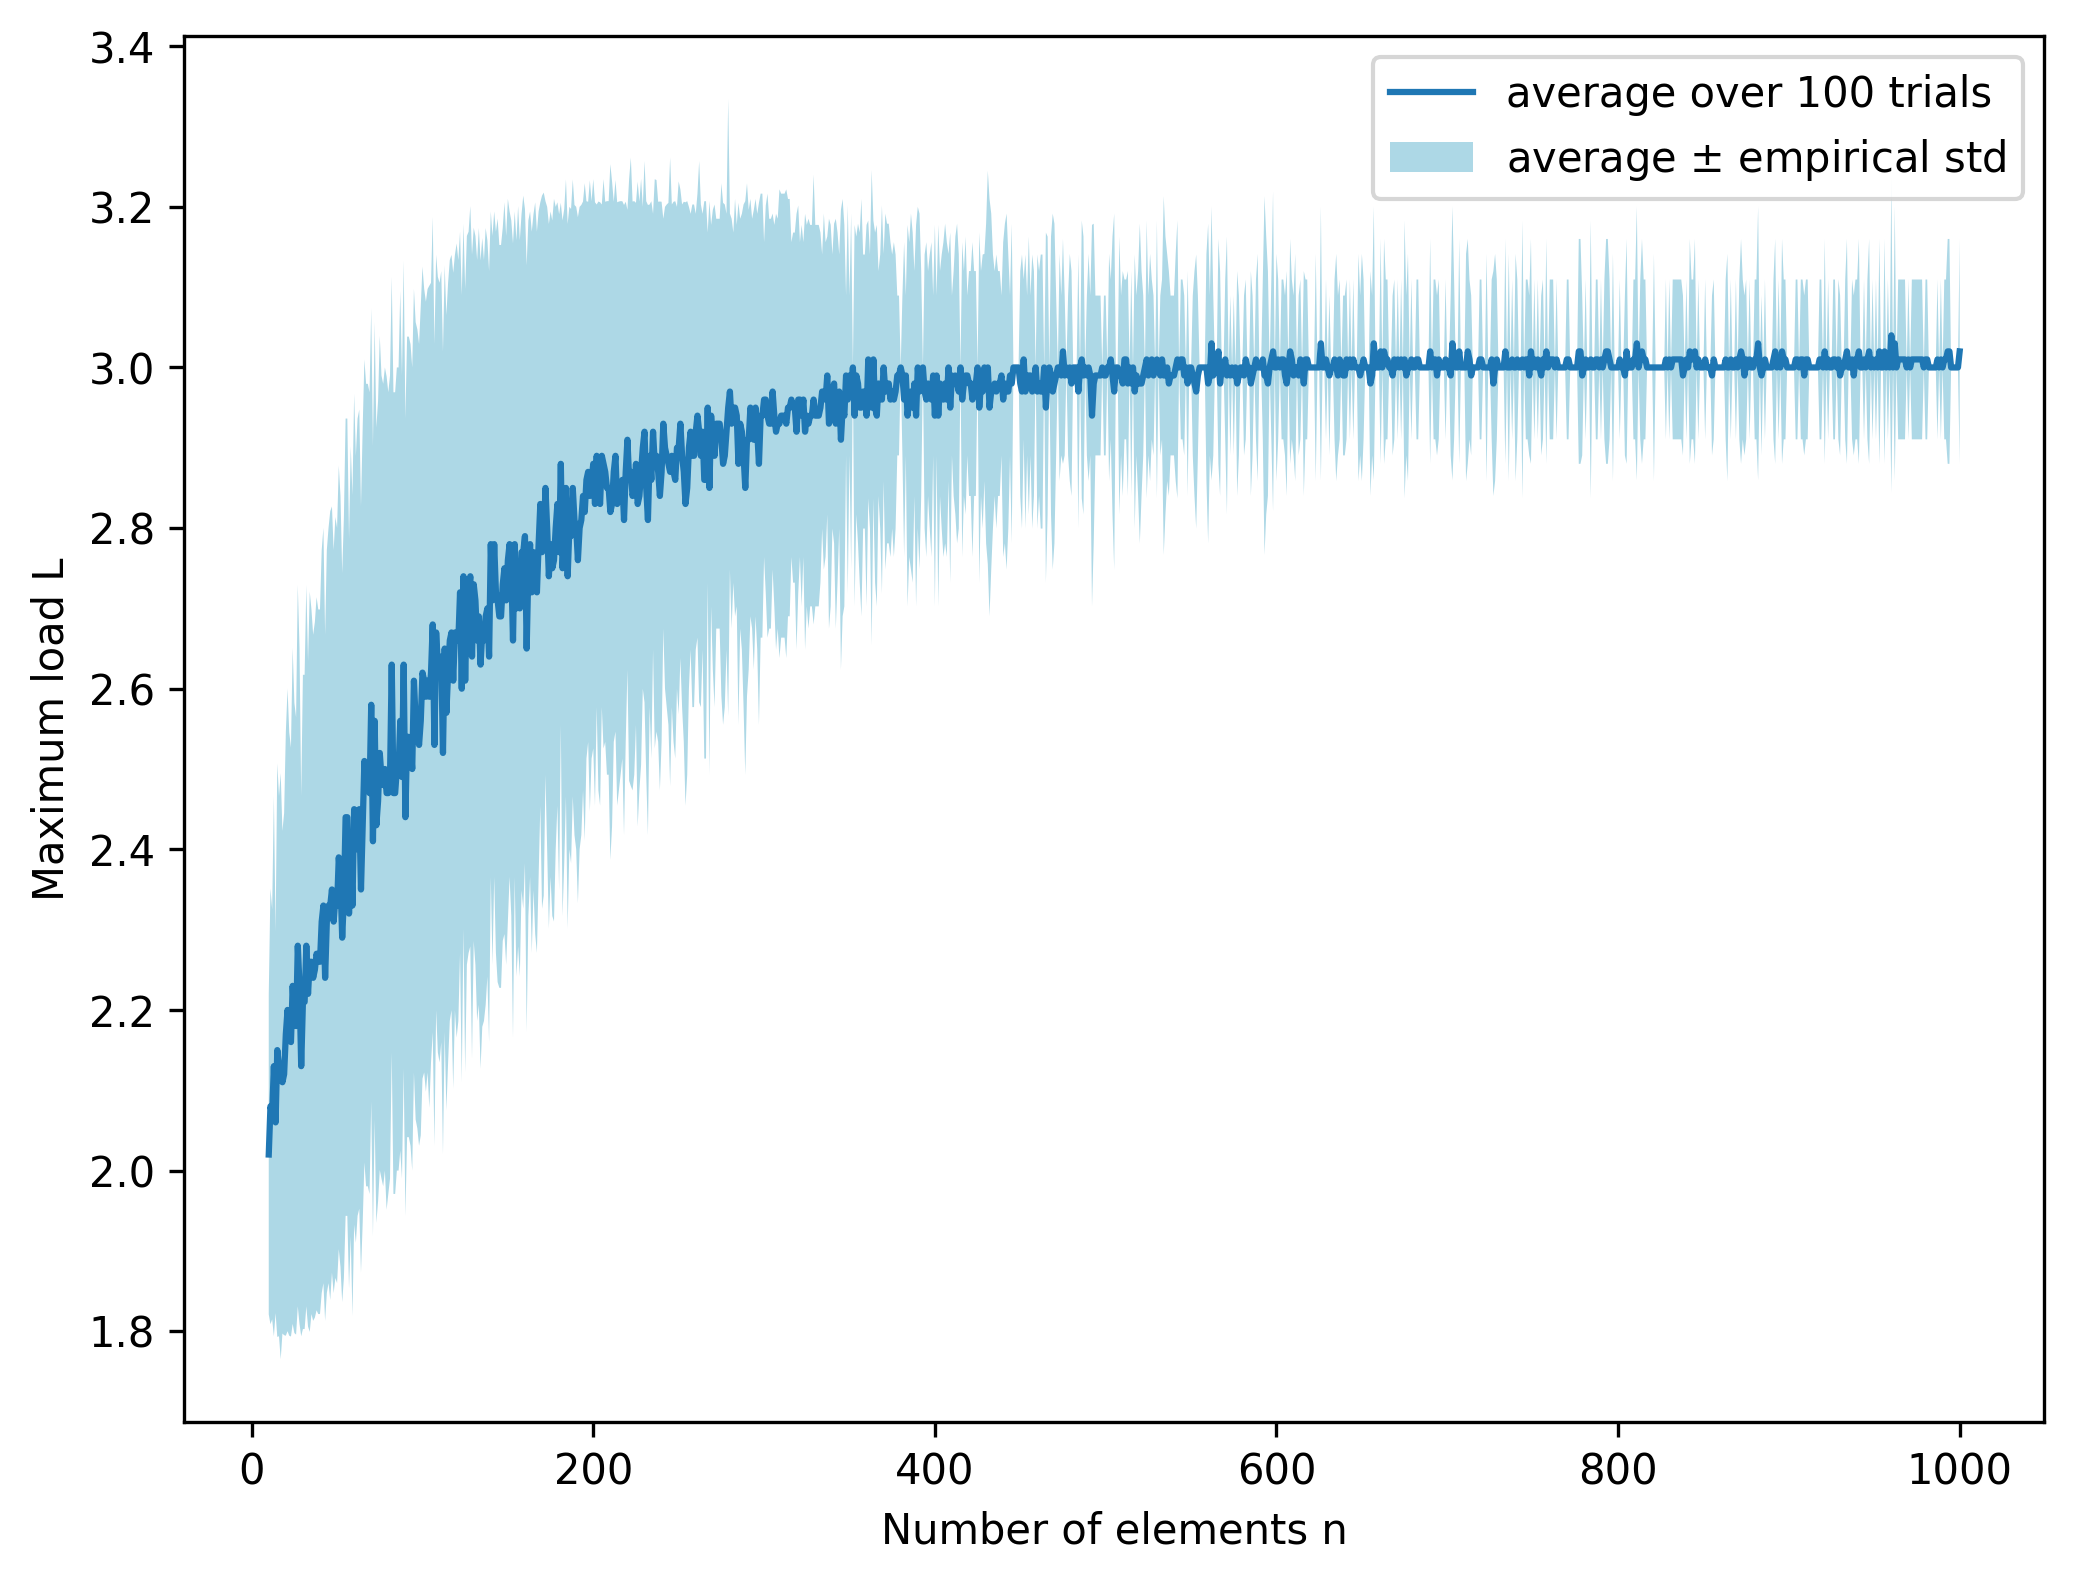
\includegraphics[width=0.9\textwidth]{figures/fig-maxload2choices.png}
\caption{Average (over 100 trials) of the maximum load when throwing $\nbins$ balls into $\nbins$ bins, using the ``best of two bins'' strategy for each bin, as a function of $\nbins$. The range given by one empirical standard deviation is plotted alongside.}
\end{figure}

Looking at the graph (\cref{fig:maxload:2}), we can see that with this ``best of two choices'' the maximum load grows much slower (as a function of $\nbins$) than in the previous setting (\cref{fig:maxload:1}). But how much slower? %How does $\orange{\hat{L}}(\nbins)$ behaves?
\begin{itemize}
    \item $\Theta(\sqrt{\log\nbins})$?
    \item $\bigTheta{\frac{\log\nbins}{(\log\log\nbins)^2}}$?
    \item $\Theta(\log\log\nbins)$?
    \item Something else?
\end{itemize}
\marginnote{\TODO{} in class: Visualization of the maximum load as $\nballs$ increases, i.e., as more balls are thrown (same with power of two choices).}

\noindent Amazingly, this simple ``power of two choices'' brings the expected maximum load from $\bigTheta{\frac{\log\nbins}{\log\log\nbins}}$ to something \emph{exponentially smaller}:
\begin{theorem}
    \label{theo:maxload:twochoices}
    The expected maximum load $\orange{\hat{L}}(\nbins)$ when throwing independently $\nbins$ balls into $\nbins$ bins using the ``best of two choices'' strategy above grows as
    \[
        \orange{\hat{L}}(\nbins) = \log\log\nbins + O(1)\,.
    \]
\end{theorem}
\noindent(We will not prove this theorem in the lecture.)

\chapter{Lecture 4: Derandomisation}
Sometimes, having a randomised algorithm is wonderful, but what we really need is a \emph{deterministic} version that achieves the same guarantees, but without the drawback of randomness: that is, we want the output to \emph{always} be good (unlike Monte Carlo-type algorithms), and the running time to \emph{always} be bounded (unlike Las Vegas-type algorithms). That is, we would like to be able, given any randomised algorithm $\Algo$, to ``derandomise'' it into an equally-good (or not much worse) deterministic version $\Algo'$. \emph{Can we achieve that?}

Unsurprisingly, the answer is a resounding ``we don't know.''\marginnote{This is actually very much tied to one of the central questions in computational complexity, the $\textsf{P}$ vs. $\textsf{BPP}$ question.} However, we do have some (limited) techniques to do so, in particular cases. Here, we will see two of them: the \emph{small random seed approach} and the \emph{method of conditional expectations}.

To illustrate this, we will consider as running example the ``maximum cut'' question:
\begin{framed}
\noindent \textsc{Max-Cut}: Given an (undirected) graph $G=(\red{V},\orange{E})$ on $\red{n}$ vertices and $\orange{m}$ edges, output a cut $(A,B)$ (partition of $\red{V}$) \emph{maximising} the number $c(A,B)$ of edges between $A$ and $B$.
\end{framed}
Of course, we would like an efficient algorithm for that. As a baseline, one could try to ``just'' find a good algorithm to solve the problem. Unfortunately, this is very unlikely to pan out:
\begin{fact}
    $\textsc{Max-Cut}$ is NP-Hard.
\end{fact}
This is annoying, as this strongly hints we should give up on trying to find an efficient algorithm (deterministic, but, also, randomised -- this is most likely very hard too) for $\textsc{Max-Cut}$. An \emph{exact} algorithm, at least: but maybe we can get a good \emph{approximation} algorithm?\footnote{Recall that an $\alpha$-approximation algorithm is an algorithm whose output's value is within a factor $\alpha > 0$ of the optimal solution's value.}

Here is an obvious randomised algorithm: \emph{choose a cut $(A,B)$ uniformly at random.} Or, with more words and in pseudocode:
\begin{algorithm}[H]
\begin{algorithmic}[1]
        \State $(A,B) \gets (\emptyset,\emptyset)$
        \ForAll{$v\in \red{V}$}
            \State $X_v \gets \bernoulli{1/2}$ \Comment{Independent of previous choices} \label{line:random:maxcut:cointoss}
            \If{$X_v = 1$}
            add $v$ to $A$
            \Else\ 
            add $v$ to $B$
            \EndIf
        \EndFor
        \State \Return $(A,B)$
    \end{algorithmic}
    \caption{Randomised algorithm for $\textsc{Max-Cut}$.}
    \label{algo:random:maxcut}
\end{algorithm}
\emph{Is it any good?} Maybe surprisingly, not too bad: in expectation, what it returns is a cut with at least \emph{half} as many edges as the best possible:
\begin{theorem}
    \label{theo:expected:maxcut}
    For every $G=(V,E)$, the output $(A,B)$ of ~\cref{algo:random:maxcut} satisfies 
    \[
    \bEE{c(A,B)} \geq \frac{1}{2}\orange{m} \geq \frac{1}{2}\operatorname{OPT}(G)\,.
    \]
    Moreover, the algorithm runs in time $\bigO{\red{n}}$.
\end{theorem}
\begin{proof}
    The proof is immediate by linearity of expectation. Fix any edge $e\in \orange{E}$ and let $X_e$ denote the indicator random variable ``$e$ is a cut edge'' (that is, one end is in $A$, the other in $B$). It is easy to check that $\bEE{X_e}=1/2$ (both endpoints are in $A$ with probability $1/2\cdot 1/2=1/4$, same for both endpoints in $B$, so an edge crosses with probability $1/2$).

Rewriting $c(A,B)=\sum_{e\in E} X_e$, by linearity of expectation, we get
\[
\bEE{c(A,B)} = \bEE{\sum_{e\in \orange{E}} X_e}= \sum_{e\in \orange{E}}\bEE{X_e} =  \sum_{e\in \orange{E}}\frac{1}{2} = \frac{\orange{m}}{2}
\]
and the last part of the statement follows from observing that the best possible cut cannot have more than $\orange{m}$ edges.
\end{proof}

Can we convert~\cref{algo:random:maxcut} into a \emph{deterministic} (and still efficient) algorithm?

%%%%%%%%%%%%%%%%%%%%%%%%%%%%%%%%%%%%%%%%%%%%%%%%%%%%
\section{Method 1: derandomizing the random seed}
Let us get back to the view of a randomized algorithm from the first lecture, as an ``algorithm $\Algo$ taking an input $x$ and a string of uniformly random bits $\green{r}\in\{0,1\}^\ast$.'' Imagine (1)~$\Algo$ has a positive probability of returning a good solution; (2)~we have a worst-case bound $\green{R}$ on the \emph{randomness complexity} of our algorithm, \ie on the maximum number of random bits it would every need on any input $x$; and (3)~that, given a solution $y$ to the task, that we can \emph{verify} efficiently whether $y$ is a good solution~--~say, by running another algorithm $\orange{V}$ on $(x, y)$.

Then the claim is that the following algorithm is a deterministic algorithm that finds a good solution:
\begin{algorithm}[H]
\begin{algorithmic}[1]
        \Require Input $x$
        \ForAll{$\green{r}\in\{0,1\}^{\green{R}}$}
            \State $y \gets \Algo(x; \green{r})$ \Comment{Run $\Algo$ on $x$ with randomness $\green{r}$}
            \If{$V(x,y) = 1$} \Comment{Verify if $y$ is a good solution}
              \State\Return $y$ \Comment{If so, we are done}
            \EndIf
        \EndFor
    \end{algorithmic}
    \caption{Derandomization approach (by brute-forcing over the random seed)}
    \label{algo:random:derandom:1}
\end{algorithm}
The fact that~\cref{algo:random:derandom:1} always returns a good solution, under our assumptions (1), (2), and (3), is immediate: there exists \emph{some} choice of the randomness $\green{r}$\marginnote{Importantly, this ``good random seed'' $\green{r}$ may not be the same for all $x$.} for which $\Algo$ returns a good solution on input $x$; once we try this particular $\green{r}$ in the loop, then we get a good solution $y$, and the verifier $\orange{V}$ successfully detects it. 

There is, of course, a catch:
\begin{fact}
    \label{fact:derandomization:smallseed}
    \cref{algo:random:derandom:1} runs in time $2^{\green{R}}\Paren{T_{\Algo}+T_{\orange{V}}}$, where $T_{\Algo},T_{\orange{V}}$ are the running times of the algorithm $\Algo$ and verifier $\orange{V}$.
\end{fact}
In particular, given that $\green{R}$ could be quite large (the only \emph{a priori} bound we have is $\green{R} \leq T_{\Algo}$),\marginnote{Can you see why?} this could be really bad \emph{even if $\Algo$ and $\orange{V}$ are efficient}: exponential in the input size, or even worse.

\paragraph{So what to do?} One hope we may have is to get a much better bound on $\green{R}$ for some specific algorithms, or even to slightly modify these algorithms to make sure $\green{R}$ is small. For instance, if we can design a randomised algorithm which only needs say $\green{R} \leq 2\log n$ bits of randomness on inputs of size $n$, then we get $2^{\green{R}} = n^{2}$: that's polynomial!

Looking back at~\cref{algo:random:maxcut}, it \emph{seems} like we are using an awful number of random bits: one for each vertex $v\in \orange{V}$, so $\green{R} = \red{n}$ in total. That is definitely not great. And yet, do we actually \emph{need} this many independent random bits? Could we do with a much smaller number and use something like hash functions?\marginnote{Hash functions are essentially magic: when you know how to use them, they are incredible. When you don't, you end up with a third arm growing out of your ear.}

The only part of the proof of~\cref{theo:expected:maxcut} where we used the randomness was to argue that each edge $e=(u,v)$ is a cut-edge with probability $1/2$. This argument requires independence of the two random bits involved: the random bit $B_u$ for $u$, and the random bit $B_v$ for vertex $v$. That is all: 
\begin{framed}
\noindent\emph{As long as $B_u$ and $B_v$ are independent for each of the $\binom{\red{n}}{2}$ pairs of distinct vertices $(u,v)$, the proof goes through!}
\end{framed}
That is called \emph{pairwise independence}, and this is a \emph{much} weaker requirement than (full) independence. In particular, we can use good hash functions to get pairwise independence very cheaply~--~to see how, let us introduce a key definition:\marginnote{Importantly, here $x,x',y,y'$ are not random! We pick a hash function $\green{h}$ at random and see where it sends the inputs. So $\green{h}$ is a \emph{randomly picked hash function} (among the $\abs{\green{\mathcal{H}}}$ choices), not a ``random function'': once $\green{h}$ is picked, there is nothing random anymore.}
\begin{definition}
    \label{def:universal:pairwise:hash}
    A family of functions $\green{\mathcal{H}} \subseteq \{h\colon \cX \to \cY\}$ is a \emph{family of pairwise independent hash functions},  or a \emph{strongly universal hash family}, if, for every $x,x'\in \cX$ with $x\neq x'$ and every $y,y'\in\cY$,
    \[
        \probaDistrOf{\green{h}\sim \green{\mathcal{H}}}{ \green{h}(x) = y, \green{h}(x') = y' } = \frac{1}{\abs{\cY}^2}
    \]
    where the probability is over the uniformly random choice of~$\green{h}\in\green{\mathcal{H}}$.
\end{definition}
Why does that help? Take the example of $\cX=[\red{n}]$ and $\cY=\{0,1\}$ in the definition above. Picking a hash function $\green{h}\in\green{\mathcal{H}}$ uniformly at random only takes $\log\abs{\green{\mathcal{H}}}$ truly independent random bits. But with these $\log\abs{\green{\mathcal{H}}}$ random bits, we obtain $|\cX|=\red{n}$ random bits
\[
    \green{h}(1), \green{h}(2), \dots, \green{h}(\red{n}) \in \{0,1\}
\]
which are \emph{not} fully independent, but such that \emph{any two of them behaves exactly like a pair of uniformly random bits.} This is exactly what we need! The only missing part is: \emph{do there exist ``small''\marginnote{Small enough, because we want to use as few ``true'' random bits as possible, and that will cost us $\log\abs{\green{\mathcal{H}}}$ of them.} families of pairwise independent hash functions $\green{\mathcal{H}} \subseteq \{h\colon [\red{n}] \to \{0,1\}\}$?} 

\begin{fact}
    \label{fact:pairwise:hash:functions}
    There exists an explicit\footnote{Easy to construct and use. We will prove it in the tutorial!} family of pairwise independent hash functions $\green{\mathcal{H}} \subseteq \{h\colon [\red{n}] \to \{0,1\}\}$ with $\abs{\green{\mathcal{H}}} = 2^{\clg{\log(\red{n}+1)}}$.
\end{fact}

This is great news! Now we can modify~\cref{algo:random:maxcut} to first pick $\green{h}$ uniformly at random from this specific $\green{\mathcal{H}}$ (this only requires $\green{R} \leq \clg{\log(\red{n}+1)}$ bits of randomness), and then use $X_v \gets \green{h}(v)$ as random coin toss for vertex $v$ in~\cref{line:random:maxcut:cointoss}. 

\begin{algorithm}[H]
\begin{algorithmic}[1]
        \State $(A,B) \gets (\emptyset,\emptyset)$
        \State Draw $\green{h}\colon \red{V} \to \{0,1\}$ uniformly at random from the $\green{\mathcal{H}}$ promised by~\cref{fact:pairwise:hash:functions}, using $\green{R}=\clg{\log(\red{n}+1)}$ random bits
        \ForAll{$v\in \red{V}$}
            \State $X_v \gets \green{h}(v)$ \Comment{Pairwise independence}
            \If{$X_v = 1$}
            add $v$ to $A$
            \Else\ 
            add $v$ to $B$
            \EndIf
        \EndFor
        \State \Return $(A,B)$
    \end{algorithmic}
    \caption{(Modified) Randomised algorithm for $\textsc{Max-Cut}$ to use a small random seed.}
    \label{algo:random:maxcut:smallseed}
\end{algorithm}

By pairwise independence, the proof of correctness of this (modified)~\cref{algo:random:maxcut} goes through exactly as in~\cref{theo:expected:maxcut}, but now we use much fewer random bits\dots So, when derandomising the algorithm \emph{via}~\cref{algo:random:derandom:1}, we only pay a factor
\[
    2^{\green{R}} = 2^{\clg{\log(\red{n}+1)}} \leq 2(\red{n}+1) = O(\red{n})
\]
What about the rest? Well, we saw already that $T_{\Algo}=O(\red{n})$. As for the time $T_{\orange{V}}$ it takes to verify a cut $(A,B)$ has size at least $\orange{m}/2$, this is $T_{\orange{V}} = O(\orange{m}+\red{n})$, and so by~\cref{fact:derandomization:smallseed} our ``derandomised algorithm'' has running time at most
\[
    2^{\green{R}}\Paren{T_{\Algo}+T_{\orange{V}}} = \bigO{\red{n}(\orange{m}+\red{n})}\,.
\]
Not bad. But we are missing a small part: one of the assumptions required to derandomise using~\cref{algo:random:derandom:1} was ``(1)~$\Algo$ has a positive probability of returning a good solution.'' We never checked this: all we know is that our randomised algorithm, \cref{algo:random:maxcut:smallseed}, returns a solution that is good (\ie with value at least $\frac{1}{2}\orange{m}$) \emph{in expectation}. Does that mean it has a \emph{positive probability} of returning a good solution?

\noindent Thankfully, yes: it can be arbitrarily small, but it is positive:\marginnote{Put differently: ``a random variable cannot \emph{always} be strictly below its expectation.''}
\clearpage
\begin{fact}
    \label{fact:sometimes:at:least:expectation}
    If $X$ is a random variable such that $\expect{X}$ exists, then $\probaOf{X \geq \expect{X}} > 0$.
\end{fact}
\begin{proof}
    Given a random variable $X$ with finite expectation $\mu \eqdef \bEE{X}$, we have
$\indic{X < \mu} + \indic{X \geq \mu }= 1$. If $\probaOf{X < \mu} = 1$; then
\begin{align*}
\mu &= \bEE{X} = \bEE{X\indic{X < \mu}} + \bEE{X\indic{X \geq\mu}} \\
&< \bEE{\mu\indic{X < \mu}} + \bEE{X\indic{X \geq \mu}} \\
&\leq \underbrace{\mu \probaOf{X < \mu}}_{\leq \mu} + \bEE{X\indic{X \geq \mu}} \,.
\end{align*}
As $\probaOf{X \geq \mu} = 0$ we have $\indic{X \geq \mu}=0$ (always), so the second term is zero; and as a result we get $\mu < \mu$, a contradiction.
\end{proof}
Putting it all together, what we have done is going from~\cref{algo:random:maxcut} (randomised algorithm) to~\cref{algo:random:maxcut:smallseed} (randomised algorithm using much fewer random bits) to a deterministic algorithm (using the general technique of~\cref{algo:random:derandom:1}). This establishes the following:
\begin{theorem}
    \label{theo:expected:maxcut:derandomized:1}
    There exists a \emph{deterministic} algorithm $\Algo'$ for $\textsc{Max-Cut}$ such that, for every $G=(V,E)$, the output $(A,B)$ of$ \Algo'$ satisfies 
    \[
        c(A,B) \geq \frac{1}{2}\orange{m} \geq \frac{1}{2}\operatorname{OPT}(G)\,.
    \]
    Moreover, the algorithm runs in time $\bigO{\red{n}\max(\orange{m},\red{n})}$.
\end{theorem}


%%%%%%%%%%%%%%%%%%%%%%%%%%%%%%%%%%%%%%%%%%%%%%%%%%%%
\section{Method 2: the method of conditional expectations}

In some cases, the algorithm \emph{does} need a lot of random bits, and there is no clear way to bring the randomness complexity $\green{R}$ down. In these cases, there is (sometimes) an other option to use: the \emph{method of conditional expectations},\footnote{This is also sometimes called the method of conditional probabilities.} which we will see now in the context of our randomised algorithm for \textsc{Max-Cut},~\cref{algo:random:maxcut}.

The method of conditional expectations essentially consists in looking at the sequence of random choices our algorithm made, and replacing these random choices one by one with deterministic choices which are always ``at least as good as what the random choice would give in expectation.''

Specifically, our randomised algorithm flips one coin per vertex, and the way we wrote it in~\cref{algo:random:maxcut} it is doing so one vertex at a time.\footnote{Note that in~\cref{algo:random:maxcut}, and~\cref{algo:random:maxcut:smallseed}, we could actually make all these random choices in parallel. With this method though, we will need to make our choices sequentially.} Instead of flipping a coin, make the best \emph{greedy} decision for the current bit to choose. For simplicity, let's order the vertices as $v_1, v_2, \dots, v_{\red{n}}$, and write $X_i \in \{0,1\}$ for the bit $X_{v_i}$ that tells us if $v_i \in A$.

What we will do first is set $X_1$ deterministically, say, without loss of generality, to $1$. Then we will choose $X_2$ to ensure whatever choice we make \emph{does not decrease} the expectation of $c(A,B)$ (over the remaining choices $X_3,\dots, X_{\red{n}}$, \emph{if} we were to choose those uniformly at random). That is, we want to find an (efficiently computable, and deterministic) rule that tells us how to set $X_{i+1}$ based on our previous choices $X_1,\dots, X_i$, which would ensure that the conditional expectation of $c(A,B)$ does not decrease:
\begin{equation}
    \label{eq:method:conditional:expectations}
	\expectCond{c(A,B) }{X_1,\dots, X_i} \stackrel{\rm want}{\leq} \expectCond{c(A,B) }{X_1,\dots, X_{i+1}}
\end{equation}
If we had that, we would be in good shape, since then
\begin{align*}
	\frac{\orange{m}}{2} &= \expect{c(A,B) } \\
    &\leq \expectCond{c(A,B) }{X_1}  \\
    &\leq \expectCond{c(A,B) }{X_1,X_2}  \\
    &\leq \dots  \\
    &\leq \expectCond{c(A,B) }{X_1,X_2,\dots, X_{\red{n}}} 
\end{align*}
and that very last term is the value of the cut we finally obtain once we have (deterministically) chosen $X_1,X_2,\dots, X_{\red{n}}$: there is no randomness left or choice remaining to make, we just have our cut $(A,B)$!

So \emph{how} do we do this ``derandomisation''? What is the rule we should follow to choose $X_{i+1}$ based on previous choices in order to guarantee~\eqref{eq:method:conditional:expectations} holds? Observe that, for any given $1\leq i\leq \red{n}-1$, 
\begin{align*}
		&\expectCond{c(A,B) }{X_1,\dots, X_i} \\
		&\quad= \probaOf{\blue{X_{i+1}=0}}\expectCond{c(A,B) }{X_1,\dots, X_i, \blue{X_{i+1}=0}} \\
		&\qquad\qquad+ \probaOf{\red{X_{i+1}=1}}\expectCond{c(A,B) }{X_1,\dots, X_i, \red{X_{i+1}=1}} \\
		&\quad= \blue{\frac{1}{2}}\expectCond{c(A,B) }{X_1,\dots, X_i, \blue{X_{i+1}=0}}
		+ \red{\frac{1}{2}}\expectCond{c(A,B) }{X_1,\dots, X_i, \red{X_{i+1}=1}} \\
		&\quad\leq \max\Paren{\expectCond{c(A,B) }{X_1,\dots, X_i, \blue{X_{i+1}=0}} ,\expectCond{c(A,B) }{X_1,\dots, X_i, \red{X_{i+1}=1}} }
\end{align*}
where the last inequality uses that $\frac{x+y}{2} \leq \max(x,y)$. So \emph{if} we had a way to efficiently compute the two quantities 
\[
    \expectCond{c(A,B) }{X_1,\dots, X_i, \blue{X_{i+1}=0}}
\]
and 
\[
    \expectCond{c(A,B) }{X_1,\dots, X_i, \red{X_{i+1}=1}}
\]
we could just greedily pick the choice of $X_{i+1}$ corresponding to the maximum of the two, and we would be done.\footnote{Technically, we don't even need to compute the two values, we just need to have a way to figure out which one of the two is largest.}

Luckily: here, we can. Let's take a step back: once we have already chosen $X_1,\dots, X_i$, we have decided where to put the first $i$ vertices $v_1,\dots, v_i$: either in $A$, or not. Then, our choice for $X_{i+1}$ can only affect the edges with one endpoint being $v_{i+1}$, so our decision can only impact two types of edges, depending on where their \emph{other} endpoint is:\marginnote{Phrased differently: at any given stage, $c(A,B)$ is the sum of the contribution of the edges already committed to (both endpoint vertices have been assigned to $A,B$), and those still open (at least one vertex endpoint not decided yet). The first contribution is fixed, and the expectation of the second is still $\frac{1}{2}$ for each edge.}
\begin{itemize}
	\item that endpoint is a vertex in $v_1,\dots, v_i$: our choice for $v_{i+1}$ will fully determine whether these edges contribute to $c(A,B)$ or not.
	\item that endpoint is a vertex in $v_{i+2},\dots, v_{\red{n}}$: our choice for $v_{i+1}$ will leave open whether these edges contribute to $c(A,B)$. That decision will only be made in the future, separately for each of these edges, when making the choice of whether to put that second endpoint into $A$.
\end{itemize}
When we set $X_{i+1}$, we only ``commit'' on the edges of the first type, \emph{and that's all}. Therefore, the best rule is to choose $X_{i+1}$ (whether to put $v_{i+1}$ in $A$) in order to maximise the number of edges of the first kind that contribute to $c(A,B)$. This is easy to do in $O(\green{m})$ time: for each of the two options for $X_{i+1}$, count the number of edges of the form $(v_j, v_{i+1})$ with $1\leq j\leq i$ that would contribute to the cut:
\begin{align}
    \red{N_A(i+1)} &= \abs{\setOfSuchThat{1\leq \orange{j}\leq i}{ (v_{\green{j}}, v_{i+1}) \in E \text{ and } v_{\orange{j}} \in B } } \label{eq:maxcut:NAi}\\
    \blue{N_B(i+1)} &= \abs{\setOfSuchThat{1\leq \orange{j}\leq i}{ (v_{\green{j}}, v_{i+1}) \in E \text{ and } v_{\orange{j}} \in A } }  \label{eq:maxcut:NBi}\\
\end{align}
and pick whichever of the two options for which that number is the biggest! This will ensure~\eqref{eq:method:conditional:expectations} holds.

\begin{algorithm}[H]
\begin{algorithmic}[1]
        \State $(A,B) \gets (\emptyset,\emptyset)$
        \State Order the vertices as $v_1,\dots,v_{\red{n}}$ (arbitrarily)
        \ForAll{$1\leq i\leq \red{n}$}
            \State Compute $\red{N_A(i)}, \blue{N_B(i)}$ as in~\cref{eq:maxcut:NAi,eq:maxcut:NBi}
            \If{$\red{N_A(i)}\geq \blue{N_B(i)}$}
            add $v_i$ to $A$
            \Else\ 
            add $v_i$ to $B$
            \EndIf
        \EndFor
        \State \Return $(A,B)$
    \end{algorithmic}
    \caption{Derandomised algorithm for $\textsc{Max-Cut}$ using the method of conditional expectations.}
    \label{algo:random:maxcut:conditionalexpect}
\end{algorithm}

Overall, what we have shown is the following:
\begin{theorem}
    \label{theo:expected:maxcut:derandomized:2}
    There exists a \emph{deterministic} algorithm $\Algo''$ (\cref{algo:random:maxcut:conditionalexpect}) for $\textsc{Max-Cut}$ such that, for every $G=(V,E)$, the output $(A,B)$ of$ \Algo''$ satisfies 
    \[
        c(A,B) \geq \frac{1}{2}\orange{m} \geq \frac{1}{2}\operatorname{OPT}(G)\,.
    \]
    Moreover, the algorithm runs in time $\bigO{\red{n}\orange{m}}$.
\end{theorem}


\begin{framed}
\noindent We have seen two general derandomisation techniques:
\begin{itemize}
    \item If we can show our randomised algorithm uses at most $\green{R}$ truly uniformly random bits \emph{and} any that given solution can be efficiently checked, then~\cref{fact:derandomization:smallseed,algo:random:derandom:1} provide a way to get a deterministic algorithm ``almost as good'', at the cost of a factor $2^{\green{R}}$ in the time complexity.
    \item Looking at the analysis of the algorithm, we can often achieve the first point by using \emph{hash functions} (only requiring a small truly random seed), provided that the analysis only uses pairwise, or, more generally, $k$-wise independence.
    \item If our algorithm has some nice properties (namely, if can efficiently compute the \emph{conditional expectation} of our solution's value given any setting of choices made so far), then the method of conditional expectations provides another powerful way of derandomising algorithms.
\end{itemize}
\end{framed}

\paragraph{A further remark.} Everything we have said about $\textsc{Max-Cut}$ in this chapter (and our algorithms) generalises to weighted graphs (and weighted cuts). \marginnote{Try it!}

\begin{fact}
    We can do better than $1/2$! There exists an $0.878$-approximation algorithm -- just not as simple. See Section~6.2 of~\cite{WilliamsonS}. We believe this is optimal, assuming something called the ``Unique Games Conjecture'' (UGC): but even without UGC, it is known we cannot do better than $16/17\approx 0.94$ unless $\textsf{P}=\textsf{NP}$.
\end{fact}

%%%%%%%%%%%%%%%%%%%%%%%%%%%%%%%%%%%%%%%%%%%%%%%%%%%%
\section{A detour: the Probabilistic Method}
Our example above with the first method\footnote{When we used~\cref{fact:sometimes:at:least:expectation} to convert the expected guarantee into a non-zero probability of a good output.} can be viewed an instance of a general proof technique called the \emph{probabilistic method}. Namely, to prove existence of something (\eg a solution to a problem satisfying some nice properties (``there exists a maximum flow with integral flows''), or an object of a specific type (``there exists a bipartite graph such that XYZ''), etc.), there are several ways: one, very convenient, is to come up with an algorithm which outputs such an object. The algorithmic does not need to be efficient: if it outputs something of a particular type, then such things clearly must exist. This is a \emph{constructive} way to establish existence.

The probabilistic method... doesn't do that. Instead, to prove that there exists some object $x$ (in a big set $\cX$) which satisfies some ``good'' property $P(x)$, we define a probability distribution $D$ over $\cX$, and then argue that 
\begin{equation}
    \probaDistrOf{\mathbf{x}\sim D}{P(\mathbf{x}) \text{ holds}} > 0
\end{equation}
that is, an object $\mathbf{x} \in \cX$ chosen \emph{at random} according to $D$ has a non-zero (maybe very small! But non-zero) probability of being ``good.'' Well, if a randomly chosen object happens to be good with some non-zero probability, that means there must exist \emph{some} good objects\dots

The key here is to choose a suitable probability distribution $D$ over $\cX$. This is a bit of an art, but often (when $\cX$ is a finite set) considering the uniform distribution over $\cX$ works.\medskip

\noindent Here is an example: given a graph $G=(V,E)$, a 2-colouring of the edges of $G$ is a mapping $c\colon E \to \{\blue{\sf{}blue}, \red{\sf{}red}\}$. Given a colouring of the graph, a set of vertices $S\subseteq V$ is said to be \emph{monochromatic} if all the edges between vertices of $S$ have the same color: $c(e) = \red{\sf{}red}$ for all $e\in E\cap (S\times S)$, or $c(e) = \blue{\sf{}blue}$ for all $e\in E\cap (S\times S)$.

Take the complete graph on $\red{n}$ vertices. Can we find a colouring of its edges such that no subset of 2 vertices is monochromatic (well, no)? No subset of 3 vertices? No subset of $\green{k}$ vertices? For which values of $\green{k}$ is that possible?
\begin{theorem}[A sufficient condition on $\green{k}$]
    Fix $0\leq \green{k}\leq \red{n}$ such that
    \[
            \binom{\red{n}}{\green{k}}2^{-\binom{\green{k}}{2}} < \frac{1}{2}
    \]
    Then, there exists a $2$-colouring of the edges of the complete graph $K_{\red{n}}$ such that no subset of $\green{k}$ vertices is monochromatic.
\end{theorem}
\begin{proof}
    Let's take a random colouring $c$. More precisely, let's take a \emph{uniformly} random colouring $c$: each edge $e\in E$ is $\red{\sf{}red}$ or $\blue{\sf{}blue}$ with probability $1/2$, and chosen independently from all other edge colours. We want to show that the probability (over the choice of $c$) that there is no monochromatic set of size $\green{k}$ is non-zero; equivalently, that the probability that there exists (at least) one monochromatic subset $S$ of size $\green{k}$ is strictly less than 1.

    Consider any (fixed) subset $S$ of $\green{k}$ vertices. Since $S$ has size $\green{k}$ and we start with the complete graph, there are $\binom{\green{k}}{2}$ edges between vertices of $S$; so the probability that our randomly chosen $c$ makes $S$ monochromatic is
    \begin{align*}
        \probaOf{\substack{\text{all edges are \blue{\sf{}blue} or}\\\text{ all edges are \red{\sf{}red}}} }\
        &= \probaOf{ \text{all edges are \blue{\sf{}blue} }} + \probaOf{ \text{all edges are \red{\sf{}red}} } \\
        &= \frac{1}{2^{\binom{\green{k}}{2}}}+\frac{1}{2^{\binom{\green{k}}{2}}} = \frac{2}{2^{\binom{\green{k}}{2}}}
    \end{align*}
    where we used independence of the choice across edges to get $(1/2)^{\binom{\green{k}}{2}}$. That tells us the probability that a given, fixed subset $S$ is monochromatic. So to bound the probability that this happens to \emph{at least one} of them, we use a union bound over all those subsets. There are exactly $\binom{\red{n}}{\green{k}}$ of them, so by a union bound
    \begin{align*}
        \probaOf{ \substack{\text{there is at least}\\ \text{one monochromatic}\\\text{subset of size $\green{k}$}}} 
        &= \probaOf{ \bigcup_{S: |S|=\green{k}} \{S \text{ is monochromatic}\} } \\
        &\leq \sum_{S: |S|=\green{k}} \probaOf{ S \text{ is monochromatic}}\\
        &\leq \binom{\red{n}}{\green{k}}\cdot \frac{2}{2^{\binom{\green{k}}{2}}}
    \end{align*}
    which is strictly less than $1$ whenever $\binom{\red{n}}{\green{k}}2^{-\binom{\green{k}}{2}} < \frac{1}{2}$. We are done.
\end{proof}

\medskip\noindent\textbf{Further reading:} the (excellent) book by Alon and Spencer\cite{AlonSBook}.

\chapter{Lecture 5: Graph algorithms}
In the previous chapter, we used $\textsc{Max-Cut}$ as a running example to illustrate some derandomisation techniques. In this chapter, we will again look at graph algorithms, but focusing on problems for which we \emph{know} efficient deterministic algorithms. The key message here is that randomisation does allow us to do things \emph{even more efficiently}~--~and, sometimes, to also extract theorems about graphs from our algorithms!

%%%%%%%%%%%%%%%%%%%%%%%%%%%%%%%%%%%%%%%%%%%%%
\section{Karger's Min-Cut algorithm}
We will start with a beautiful algorithm, due to Karger~\cite{Karger93} (and improved by Karger and Stein~\cite{KargerS93}), for the \emph{minimum} cut question:\marginnote{If $G$ is not connected, we can detect this in $O(\orange{m}+\red{n})$ time, and then a ``minimum cut'' is\dots{} easy to find.}
\begin{framed}
\noindent \textsc{Min-Cut}: Given an (undirected) connected graph $G=(\red{V},\orange{E})$ on $\red{n}$ vertices and $\orange{m}$ edges, output a cut $(A,B)$ (partition of $\red{V}$) \emph{minimising} the number $c(A,B)$ of edges between $A$ and $B$.
\end{framed}
Of course, we want an efficient algorithm for that. As a baseline, one could try to ``just'' find a good deterministic algorithm to solve the problem. Fortunately, we have some:
\begin{fact}
    $\textsc{Min-Cut}$ can be solved by computing $\red{n}-1$ instances of the $\textsc{Max-Flow}$ problem.\marginnote{Recall the $\textsc{Max-Flow}$ problem: given a directed weighted graph and two vertices $s$ and $t$, find a maximum feasible flow from $s$ to $t$.} This can be done is polynomial time in $\red{n}$ and $\orange{m}$ (and, actually, in time~\cite{HaoO94} $\bigO{\orange{m}\red{n}\log\frac{\red{n}^2}{\orange{m}}}$).
\end{fact}
This is annoying, as this strongly hints that, well, we're done here. However, the above algorithm is quite involved: can we do as well, or even better, with a \emph{simple} randomised algorithm?

As it turns out, \emph{yes}. Here is the gist of the algorithm: (1)~Pick an edge of the graph uniformly at random. (2)~``Merge'' its two endpoints. (3)~Repeat.

That's all! Of course, to formally describe and analyse this mind-blowingly simple algorithm, we first need to define what we mean by ``merging'' two vertices. This is an operation called \emph{contraction}:
\begin{definition}
    Let $G=(\red{V},\orange{E})$ be a multigraph\footnote{We allow parallel edges, but no self-loops. So there could be several edges between two distinct vertices $u,v$ (but none from $u$ to itself).} and $e=(u,v)\in\orange{E}$ one of its edges. The \emph{contraction of $G$ with respect to $e$}, denoted $G/e$, is the multigraph on $\abs{\red{V}}-1$ vertices defined from $G$ as follows:
    \begin{enumerate}
        \item Replace $u$ and $v$ by a single vertex, $uv$;
        \item Replace all edges of $\orange{E}$ of the form $(u,w)$ or $(v,w)$ by an edge $(uv,w)$;
        \item Remove all self-loops $(uv, uv)$ the second step may have created.
    \end{enumerate}
\end{definition}
The process is illustrated in~\cref{fig:karger:contraction}. Note that a contraction can be performed in time $O(\red{n})$ given either the adjacency list or adjacency matrix representation of the multigraph.
\begin{figure}[htbp]
    \centering
    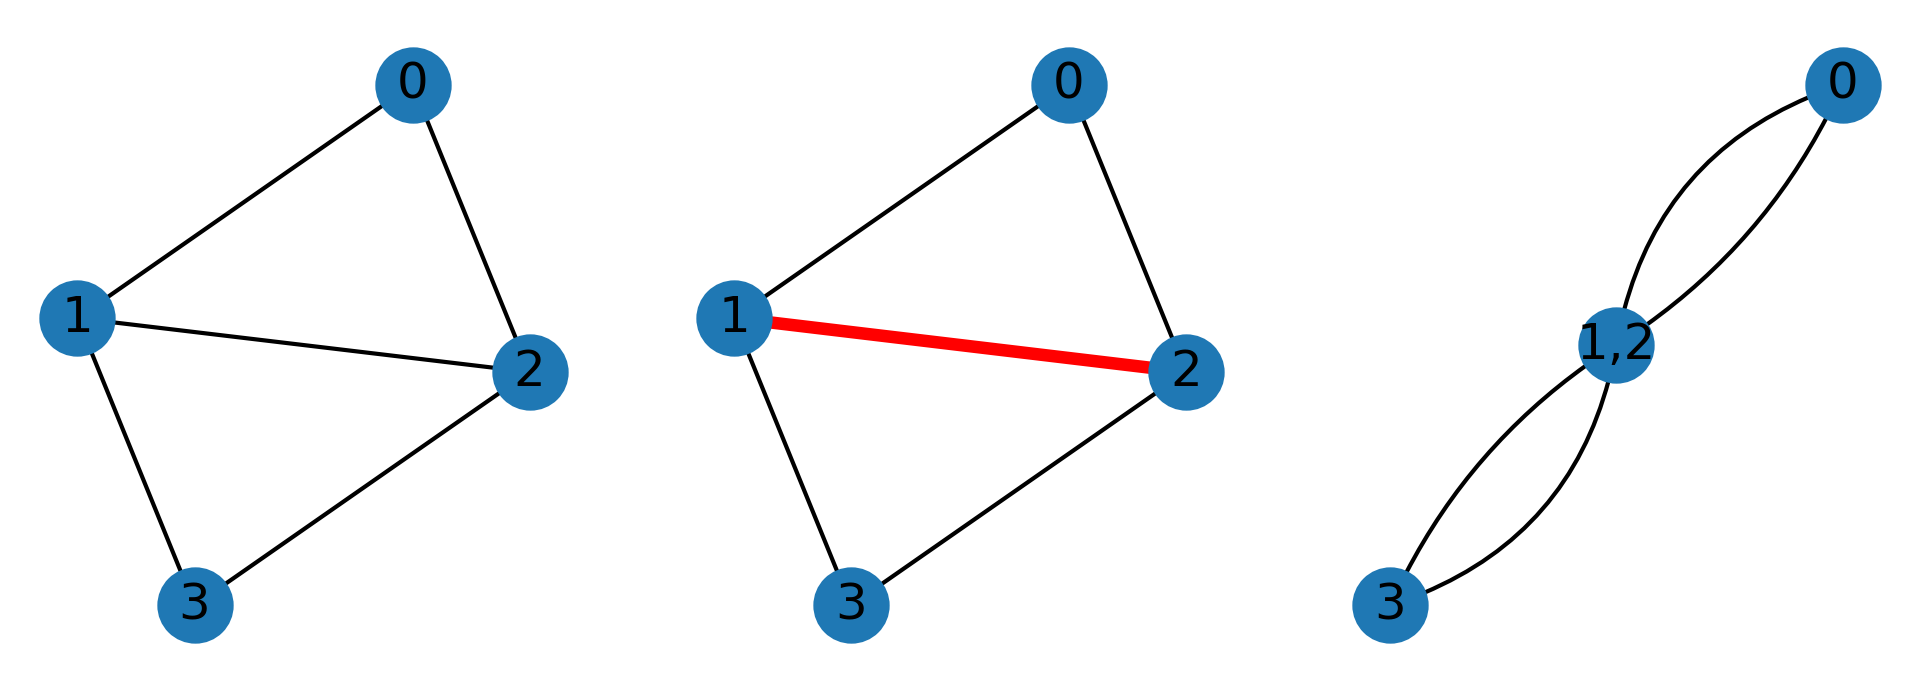
\includegraphics[width=1.0\textwidth]{figures/fig-karger-contraction.png}
    \caption{A contraction of the edge $e=(1,2)$: the original (multi)graph is on the left, and the resulting (multi)graph $G/e$ on the right.}
    \label{fig:karger:contraction}
\end{figure}

Another way to interpret the contraction is that, after contracting some edges to get a multigraph $G'=G/(e_1,\dots, e_k)$, each vertex $u$ in $G'$ corresponds to a subset of vertices $S_u\subseteq \red{V}$ from the original graph $G=(\red{V}, \orange{E})$: the subset of all vertices that were contracted together to become $u$. And any two distinct $u,v$ from $G'$ correspond to \emph{disjoint} subsets $S_v,S_v\subseteq \red{V}$ (during a contraction, a vertex cannot be merged to two separate new vertices!). 

So if after a sequence of contractions we end up with a multigraph $G'$ which has only \emph{two} vertices $u,v$, we get a cut in our original graph $G$: the cut $(S_u, S_v)$. And the value $c(S_u, S_v)$ of this cut is then exactly the number of parallel edges between $u$ and $v$. 

This is the basis for our algorithm, which we are now able to state:
\begin{algorithm}[H]
\begin{algorithmic}[1]
    \Require multigraph $G=(\red{V}, \orange{E})$
    \While{$\abs{\red{V}} > 2$}
        \State\label{alg:krager:randomedge} Pick an edge $e\in\orange{E}$ uniformly at random
        \State\label{alg:krager:result} Contract it, and let $G \gets G/e$
    \EndWhile
    \State\Return the cut defined by the remaining two vertices.
\end{algorithmic}
\caption{Karger's \textsc{Min-Cut} algorithm.}
\label{alg:karger}
\end{algorithm}
This is all. Each iteration of the loop takes time $O(\red{n})$\marginnote{The contraction operation does, and we will see in the tutorial that sampling an edge uniformly can be done in time $O(\red{n})$ as well.}; each contraction reduces the number of vertices by one, and we started with $\red{n}$ vertices: so we have $\red{n}-2$ iterations. Overall, running~\cref{alg:karger} takes $O(\red{n}^2)$ time. \emph{But is the cut it returns any good?} And importantly, \emph{why} would we expect to be any good?

\begin{figure}[htbp]
    \foreach \i in {0,1,...,10}{
    \includegraphics[scale=0.19]{figures/karger/plotgraph-\i.png} 
    }
    \caption{The sequence of steps for one run of Karger's algorithm (\cref{alg:karger}) on a (regular) graph with $\red{n}=12$ vertices and $\orange{m}=48$ edges. The cut returned has $8$ edges.}
\end{figure}

\paragraph{Some intuition.} As a thought experiment, consider any (fixed) cut $C=(A,B)$ of the graph. The only way $C$ will survive until the end of the algorithm (and be returned in~\cref{alg:krager:result}) is if we never contract any edge going from a vertex in $A$ to a vertex in $B$: that is, any vertex of the cut itself. Because as soon as we contract such an edge, some vertex in $A$ is merged with some vertex in $B$, and the cut $(A,B)$ does no longer exist in our new contracted multigraph. Put differently, the more edges there are between $A$ and $B$, the less likely the cut $C$ should be to make it to the end of the algorithm, and as a result, we expect ``small cuts'' (those with fewer edges crossing) to have a better probability to be returned.\marginnote{Consider a different strategy for~\cref{alg:krager:randomedge} of the algorithm, which would sample a pair of distinct vertices $(u,v)$ uniformly at random (not necessarily an edge). Would that work?} But that's exactly what we want: by definition, minimum cuts are the smallest cuts possible! So they should be the ones being the most likely to be returned by our algorithm\dots 

To make it formal, fix any \emph{minimum} cut $C=(A,B)$ of $G$, and let $\green{k}=c(A,B)$ be its value. For $1\leq i\leq \red{n}-2$, let $\mathcal{E}_i$ be the event that the edge $e$ picked in the $i$-th step of the algorithm does \emph{not} belong to our cut $C$. By the above discussion,
\begin{align*}
\probaOf{C\text{ is returned}} 
&= \proba[\mathcal{E}_1\cap \mathcal{E}_2\cap\dots \cap \mathcal{E}_{\red{n}-2}] \tag{No edge from $C$ is ever contracted}\\
&= \proba[\mathcal{E}_1]\probaCond{\mathcal{E}_2}{\mathcal{E}_1}\cdots\probaCond{\mathcal{E}_{\red{n}-2}}{\mathcal{E}_1\cap \mathcal{E}_2\cap\dots \cap \mathcal{E}_{\red{n}-1}}
\end{align*}
Based on this, what we need to conclude is to get a good lower bound on the probability
\[
    \probaCond{\mathcal{E}_{i+1}}{\mathcal{E}_1\cap \mathcal{E}_2\cap\dots \cap \mathcal{E}_{i}}
\]
for all $1\leq i\leq \red{n}-3$: then, we will multiply all of them, and hope for the best. Write $G_i = (\red{V}_i, \orange{E}_i)$ for the multigraph at the end of step $i$: so $G_0=G$, and $G_{\red{n}-2}$ is the $2$-vertex multigraph obtained at the end. The probability that an edge of $C$ is chosen in step $i+1$ to be contracted (if $C$ has survived until then, which is the event $\mathcal{E}_1\cap \mathcal{E}_2\cap\dots \cap \mathcal{E}_{i}$) is then equal to
\begin{equation}
            \frac{\green{k}}{|\orange{E}_{i}|}
\end{equation}
We need to (upper) bound this probability, and all we know is that:\begin{itemize}
    \item the number of vertices is $\abs{\red{V}_i} = \red{n}-i$;
    \item the value of any minimum cut of $G_i$ is $\green{k}$ (there is one cut of size $\green{k}$, our cut $C$ which survived so far; and there cannot be smaller cuts, as they would imply a smaller-than-minimum cut in the original graph $G$ as well).
\end{itemize}
The key observation is that the \emph{minimum degree} of $G_i$ must then be at least $\green{k}$. Otherwise, there would exist some vertex $u\in \red{V}_i$ with less than $\green{k}$ neighbours: choosing the cut $\{u\}, \red{V}_i\setminus\{u\}$ would give a cut in $G_i$ of size less than $\green{k}$. Using the Handshaking Lemma,\footnote{Which, importantly, also holds in (simple) multigraphs.} we have
\begin{equation}
    |\orange{E}_i| = \frac{1}{2}\sum_{v\in \red{V}_i} \deg v \geq \frac{1}{2}\abs{\red{V}_i}\cdot\green{k}
\end{equation}
or, equivalently,
\[
    \frac{\green{k}}{|\orange{E}_i|} \leq \frac{2}{\abs{\red{V}_i}} = \frac{2}{\red{n}-i}\,.
\]
This shows that
\begin{equation}
    \label{eq:karger:proba:failure:step}
    \probaCond{\mathcal{E}_{i+1}}{\mathcal{E}_1\cap \mathcal{E}_2\cap\dots \cap \mathcal{E}_{i}}
    = 1- \frac{\green{k}}{|\orange{E}_i|} \geq 1-\frac{2}{\red{n}-i}
\end{equation}
and as a result, ``multiplying all the conditional probabilities and hoping for the best'' gives
\begin{align}
\probaOf{C\text{ is returned}} 
&= \prod_{i=0}^{\ns-3} \probaCond{\mathcal{E}_{i+1}}{\mathcal{E}_1\cap\dots \cap \mathcal{E}_{i}} \notag\\
&\geq \prod_{i=0}^{\ns-3} \Paren{1-\frac{2}{\red{n}-i}} \notag\\
&= \prod_{i=0}^{\ns-3} \frac{\red{n}-i-2}{\red{n}-i} \notag\\
&= \prod_{j=3}^{\ns} \frac{j-2}{j} \notag\\
&= \frac{1\cdot 2\cdot 3\cdot 4 \cdots (\ns-2)}{3\cdot 4\cdot 5 \cdots \cdot (\ns-2)(\ns-1)\ns} \notag\\
&= \frac{2}{(\ns-1)\ns} \label{eq:karger:success:probability}\,.
\end{align}
What we showed is that, with probability at least $\frac{2}{(\ns-1)\ns}$, Karger's algorithm (\cref{alg:karger}) returns this specific minimum cut $C$. There may be more than one possible minimum cut, so the probability it returns \emph{some} minimum cut is at least $\frac{2}{(\ns-1)\ns}$:
\begin{theorem}
    \label{theo:karger}
    Karger's algorithm (\cref{alg:karger}) returns a minimum cut with probability at least $\frac{2}{(\ns-1)\ns} = \bigOmega{1/\ns^2}$.
\end{theorem}
On the one hand, this is great: the algorithm works! On the other hand, this is somewhat problematic: the probability of success we can guarantee is \emph{very} small. Fortunately, similarly to what we saw in Chapter~2, we can increase our probability of success by repetition, using~\cref{alg:karger} as a blackbox. That is:
\begin{algorithm}[H]
\begin{algorithmic}[1]
    \Require multigraph $G=(\red{V}, \orange{E})$, integer $\blue{T}$
    \For{$1\leq t\leq \blue{T}$} \!\Comment{Use fresh (independent) random bits for each}
        \State Run~\cref{alg:karger} on $G$, let $C_t$ be the output
    \EndFor
    \State\Return the smallest cut among all cuts $C_1,\dots, C_{\blue{T}}$ obtained
\end{algorithmic}
\caption{Amplifying the probability of Karger's \textsc{Min-Cut} algorithm via repetition.}
\label{alg:karger:repeated}
\end{algorithm}
From~\cref{theo:karger}, we know that each of the $\blue{T}$ independent repetitions of the algorithm has probability $p \geq \frac{2}{\ns(\ns-1)}$ of returning a minimum cut. And since it is returning the best cut among them,~\cref{alg:karger:repeated} will return a minimum cut unless \emph{none} of these $\blue{T}$ cuts is a minimum cut. So
\[
    \probaOf{\substack{\text{\cref{alg:karger:repeated} fails to}\\\text{ return a minimum cut}}} = \Paren{1-p}^{\blue{T}} \leq \Paren{1-\frac{2}{\ns(\ns-1)}}^{\blue{T}} \leq e^{-\frac{2\blue{T}}{\ns(\ns-1)}}
\]
where we used the inequality $1-x \leq e^{-x}$ in the end. To achieve probability of success $1-\errprob$, it suffices to choose $\blue{T}$ so that the RHS is at most $\errprob$: one can check that setting 
\[
    \blue{T} = \clg{\ns^2\ln(1/\errprob)}
\]
suffices. Overall, the running time is $O(\blue{T}\ns^2)$, showing the following:
\begin{theorem}
    \label{theo:karger:repeated}
    For any $\errprob>0$, the ``Best-of-$\blue{T}$'' version of Karger's algorithm (\cref{alg:karger:repeated}) returns a minimum cut with probability at least $1-\errprob$, and runs in time $\bigO{\ns^4\log(1/\errprob)}$.
\end{theorem}
Given how simple the algorithm is, this is quite remarkable! However, given that the (much more involved) best deterministic algorithm can find a minimum cut in time $O(\orange{m}\red{n}\log\frac{\ns^2}{\orange{m}}) = \bigO{\ns^3}$, it is natural to wonder if we can do even better. 

\subsection{Improving Karger’s algorithm: the Karger--Stein algorithm} The starting point is to note that Karger's algorithm does \emph{very} well in the first few iterations, but the guarantees degrade quickly towards the end. Again, let's look at a fixed minimum cut $C$ of size $\green{k}$: the probability to ``kill'' $C$ with the first contraction is very small, $\green{k}/\orange{m}$. At the $i$-th step, when $i$ is not too big, this is still very small: in~\cref{eq:karger:proba:failure:step}, we bounded it by
\[
    \frac{2}{\ns-i} \approx \frac{2}{\ns}
\]
All good! But at the \emph{end} of the algorithm, the last few steps, this becomes really, really bad: at the last step ($i=\ns-3$), for instance, the probability that $C$ is ``killed'' is only bounded by
\[
   \frac{2}{\ns-i} = \frac{2}{3} 
\]
This tells us that after surviving almost until the end, we can only guarantee that our minimum cut $C$ has a $33\%$ chance of surviving the very last step! And the first few contractions before that are not much better: each of them has a constant probability of killing $C$.

Based on this, it makes sense to only run Karger's algorithm for a while, and then do ``something else'' once we have contracted sufficiently many edges. This leaves two questions: (1)~When should we stop? and (2)~What should we do afterwards?

To answer the first question, we can look back at our analysis of the success probability. If we stop after $\ns-\blue{s}$ steps, we are left with $\blue{s}$ vertices, and similarly to what we did in~\cref{eq:karger:success:probability} we can guarantee that any fixed minimum cut survives with probability at least
\[
\prod_{i=0}^{\ns-\blue{s}-1} \frac{\red{n}-i-2}{\red{n}-i}
= \prod_{j=\blue{s}+1}^{\ns} \frac{j-2}{j}
= \frac{\blue{s}(\blue{s}-1)}{\red{n}(\red{n}-1)}
\]
If we choose $\blue{s} = \frac{\ns}{\sqrt{2}}+1$, we get
\[
    \probaOf{C \text{ survives these }\ns-\blue{s}\text{ steps}} \geq \frac{1}{2}\,.
\]
So this answers (1): we should stop once only $\frac{\ns}{\sqrt{2}}+1$ vertices remain. Then, even if there was only a single minimum cut $C$ in the original graph, it will have survived with probability at least $1/2$. But turning to question (2): what to do afterwards?\smallskip

We reduced the size of the problem by a constant factor, from $\ns$ vertices to $\approx \frac{\ns}{\sqrt{2}}$. In the absence of a better idea, this seems to call for a recursive approach.\marginnote{``When in doubt, recurse''}

First, the base case: we can only recurse if we make progress at each call, and that can only happen if
\[
    \clg{\frac{\ns}{\sqrt{2}}+1} > \ns
\]
and that is only true for $\ns \geq 7$. This gives us our base case: if $\ns \leq 6$, we will just compute a minimum cut by brute force (in constant time).

Second, $1/2$ probability is much better than $\approx 1/\ns^2$, but it is still small: for a recursive approach, dropping our probability of success by such a constant factor at each recursive step could be bad. But if we have a probability of success at least $1/2$, repeating the first stage \emph{twice} might not be a bad idea: we would have two different multigraphs $G_1,G_2$ on $\blue{s} \approx \frac{\ns}{\sqrt{2}}$ vertices, each of them (independently) still containing a minimum cut with probability at least $1/2$. ``In expectation'', at least $2\cdot (1/2)=1$ still will have a minimum cut. This gives us our algorithm, given in~\cref{alg:karger:stein}.
\begin{algorithm}[htbp!]
\begin{algorithmic}[1]
%%%%%%%%%%%%%%%%%%%%%%%%%%%%%%%%%%%%%%%%%%%%%%%%%%
\algblockdefx{BeginFirstStage}{EndFirstStage}{$\triangleright$~\textbf{Contraction}}{}
\algblockdefx{BeginSecondStage}{EndSecondStage}{$\triangleright$~\textbf{Recursion}}{}
\algtext*{EndFirstStage}% Remove "EndFirstStage" text and line
\algtext*{EndSecondStage}% Remove "EndSecondStage" text and line
%%%%%%%%%%%%%%%%%%%%%%%%%%%%%%%%%%%%%%%%%%%%%%%%%%
\Procedure{ModifiedKarger}{$G=(\red{V}, \orange{E})$, $\blue{s}$}
    \While{$\abs{\red{V}} > \blue{s}$}
        \State Pick an edge $e\in\orange{E}$ uniformly at random
        \State Contract it, and let $G \gets G/e$
    \EndWhile
    \State\Return $G$
\EndProcedure
\Procedure{KargerStein}{$G=(\red{V}, \orange{E})$}
    \If{$\abs{\red{V}} \leq 6$}
        \State \Return a minimum cut \Comment{Brute-force computation}
    \EndIf
    \State Set $\blue{s} \gets \clg{{\ns}/{\sqrt{2}}+1}$
    \BeginFirstStage
        \State $G_1 \gets \textsc{ModifiedKarger}(G,\blue{s})$
        \State $G_2 \gets \textsc{ModifiedKarger}(G,\blue{s})$
    \EndFirstStage
    \BeginSecondStage
        \State $C_1 \gets \textsc{KargerStein}(G_1)$
        \State $C_2 \gets \textsc{KargerStein}(G_2)$
    \EndSecondStage
    \State\label{alg:karger:stein:return}\Return the smallest cut among $C_1,C_2$
\EndProcedure
\end{algorithmic}
\caption{The Improved Karger--Stein \textsc{Min-Cut} algorithm.}
\label{alg:karger:stein}
\end{algorithm}
To analyse this \textsc{KargerStein} algorithm, we need to establish its running time $T(\ns)$ and its probability of success $p(\ns)$. The running time turns out to be the simplest: we have two calls to \textsc{ModifiedKarger}, which (as in~\cref{alg:karger}) each take time $O(\ns^2)$; following by two recursive calls on instances of size $\blue{s}\approx \ns/\sqrt{2}$. Ignoring the ceiling for simplicity, this gives the recurrence relation
\begin{equation}
    T(\ns) = 2T(\ns/\sqrt{2})+O(\ns^2)
\end{equation}\marginnote{Verify it, \eg with the Master Theorem; or, even better, without it.}
which solves to $\boxed{T(\ns)=O(\ns^2\log\ns)}$ \emph{via} the standard techniques.\medskip

The probability of success $p(\ns)$ is trickier. From our setting of $\blue{s}$, we know that $G_1$ still contains a minimum cut with probability at least $1/2$: whenever that happens, $C_1$ will be a minimum cut if the recursive call to \textsc{KargerStein} is successful, which itself happens with probability at least $p(\ns/\sqrt{2})$. That is,
\[
    \probaOf{C_1\text{ is a minimum cut}} \geq \frac{1}{2}\cdot p\Paren{\frac{\ns}{\sqrt{2}}}
\]
Similarly, looking at $G_2$ we have $\probaOf{C_2\text{ is a minimum cut}} \geq \frac{1}{2}\cdot p({\ns}/\sqrt{2})$. Since we are taking the best of $C_1,C_2$ on~\cref{alg:karger:stein:return}, the algorithm succeeds unless \emph{neither} of $C_1,C_2$ is a minimum cut:
\begin{align*}
p(\ns) &= 1-\Paren{1-\probaOf{C_1\text{ is a minimum cut}}}\Paren{1-\probaOf{C_2\text{ is a minimum cut}}} \\
&\geq 1-\Paren{1-\frac{1}{2} p\Paren{\frac{\ns}{\sqrt{2}}}}^2
\end{align*}
We are left with the task of solving this recurrence relation on $p(\ns)$, with the base cases $p(\ns) = 1$ for $\ns\leq 6$. 
\begin{claim}[\advancedstuff]
    The recurrence relation
    \[
       p(\ns) \geq 1-\Paren{1-\frac{1}{2} p\Paren{\frac{\ns}{\sqrt{2}}}}^2
    \]
    has solution $p(\ns) = \bigOmega{1/\log\ns}$.
\end{claim}
\begin{proof}
    Write $\ns = \sqrt{2}^t$ for $t\geq 1$.
    Expanding the square, this boils down to analysing the recurrence relation
    \[
        p(\sqrt{2}^t) \geq p(\sqrt{2}^{t-1}) - \frac{1}{4}p(\sqrt{2}^{t-1})^2
    \]
    or, equivalently (reparameterizing by setting $f(t) = p(\sqrt{2}^t)\in[0,1]$),
    \begin{equation}
        f(t) \geq f(t-1)-\frac{1}{4}f(t-1)^2\,.
    \end{equation}\marginnote{\advancedstuff{} Another ``rabbit-out-of-the-hat'' proof: set $g(t) = \frac{4}{f(t)}-1$, and substitute in the inequality. Solve the resulting inequality.}
    Note that the function $x\mapsto x-\frac{1}{4}x^2$ is increasing on $[0,1]$: this will come handy later. We will show by induction on $t$ that $f(t) \geq \frac{1}{t+2}$.
    \begin{itemize}
        \item This is true for $t=0$, since $f(0) = p(1)=1$.
        \item Assuming it is true for $t-1$, we have
        \begin{align*}
        f(t) &\geq f(t-1)-\frac{1}{4}f(t-1)^2 \\
        &\geq \frac{1}{t+1}-\frac{1}{4}\Paren{\frac{1}{t+1}}^2 \tag{induction hypothesis and $x\mapsto x-\frac{1}{4}x^2$ increasing} \\
        &= \frac{4t+3}{4(t+1)^2} = \frac{1}{t+2} + \frac{3t+2}{4(t+1)^2(t+2)} \\
        &\geq \frac{1}{t+2}
        \end{align*}
        concluding the induction proof.
    \end{itemize}
    Recalling that $\ns = \sqrt{2}^t$, we have $t = 2\log\ns$, and the above shows that $p(\ns) \geq \frac{1}{2\log\ns+2} = \bigOmega{\frac{1}{\log\ns}}$, as claimed.
\end{proof}
\noindent What we have shown can be summarised as follows:
\begin{theorem}
    \label{theo:karger:stein}
    The Karger--Stein algorithm (\cref{alg:karger:stein}) runs in time $O(\ns^2\log\ns)$, and returns a minimum cut with probability at least $\bigOmega{1/\log\ns}$.
\end{theorem}
Moreover, with exactly the same approach as\marginnote{Exercise: prove it!} for~\cref{theo:karger:repeated} (using~\cref{theo:karger:stein} and setting $\blue{T} = O(\log\ns\cdot \log(1/\errprob))$), we get
\begin{corollary}
    \label{theo:karger:stein:repeated}
    For any $\errprob>0$, the ``Best-of-$\blue{T}$'' version of the Karger--Stein algorithm returns a minimum cut with probability at least $1-\errprob$, and runs in time $\bigO{\ns^2\log^2\ns \log(1/\errprob)}$.
\end{corollary}
This is now typically \emph{much} faster than the $\bigO{\orange{m}\red{n}\log\frac{\red{n}^2}{\orange{m}}}$ running time of the deterministic algorithm!\marginnote{Specifically, as long as the graph is even mildly dense, \ie $\orange{m} \gg \ns\log\ns$.}

\begin{remark}
    There is a different deterministic algorithm, due to Stoer and Wagner~\cite{StoerW97} and not based on computing maximum flows, with the running time $\bigO{\orange{m}\red{n}+\red{n}^2\log\red{n}}$ (slightly better than $\bigO{\orange{m}\red{n}\log\frac{\red{n}^2}{\orange{m}}}$, but still worse than~\cref{theo:karger:repeated}). Interestingly, this algorithm also works by performing some type of contraction (merging two carefully selected vertices at each step).
\end{remark}

\subsection{How many minimum cuts are there?}
The \textsc{Min-Cut} question we have considered so far asks to \emph{find} a minimum cut in a graph $G$: \emph{any} minimum cut. There is always at least \emph{one} minimum cut, but could there be more? How many, at most?
\begin{itemize}
    \item $\Theta(\ns)$?
    \item $\Theta(\ns^2)$?
    \item $\Theta(2^{\ns})$?
    \item Something else?
\end{itemize}
And \emph{how to prove it}?\medskip

Fortunately, we already have the answer, \emph{and} done the proof. We just did not realise it at the time! This is a beautiful example where analysing an algorithm establishes a structural result, almost ``as a side effect.''

Taking a step back: in order to prove~\cref{theo:karger}, we have shown that if $C$ is a minimum cut of $G$, then~\cref{alg:karger} outputs $C$ with probability at least
\[
    \frac{2}{\ns(\ns-1)} = \frac{1}{\binom{\ns}{2}}
\]
This means that if there exists $\green{M}$ distinct minimum cuts in the graph $G$, the probability to output one of them is at least
\[
    \probaOf{ \substack{\textsc{Karger}(G)\text{ outputs}\\\text{one of } C_1,\dots, C_{\green{M}}}} = \sum_{i=1}^{\green{M}} \probaOf{ \textsc{Karger}(G)\text{ outputs } C_i} \geq \frac{\green{M}}{\binom{\ns}{2}}
\]
But probabilities are at most one, so $\probaOf{ \substack{\textsc{Karger}(G)\text{ outputs}\\\text{one of } C_1,\dots, C_{\green{M}}}}\leq 1$. Which means that
\[
    \green{M} \leq \binom{\ns}{2}
\]
and we get the following ``for free'':
\begin{theorem}
    An undirected graph $G=(\red{V},\orange{E})$ on $|\red{V}|=\ns$ vertices has at most $\binom{\ns}{2}$ minimum cuts.
\end{theorem}
This is quite surprising, since every\marginnote{Do you see why?}  graph on $\ns$ vertices has exactly $2^{\ns-1}-1$ distinct (not necessarily minimum) cuts. As usual, we can ask whether this $\binom{\ns}{2}$ bound is tight: and the answer is \emph{yes}, as there exist some $\ns$-vertex graphs with that many minimum cuts. A simple example is a cycle on $\ns$ vertices, where choosing any $2$ edges out of $\ns$ defines a distinct minimum cut: see~\cref{fig:cycle:graph}.
\begin{figure}[htbp]
    \centering
    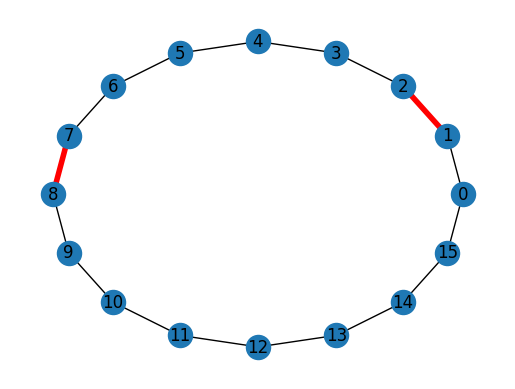
\includegraphics[width=0.9\textwidth]{figures/fig-cyclegraph}
    \caption{The cycle graph $C_{16}$ on $16$ vertices, along with a specific (mininum) cut (defined by the two \red{red} edges). Any choice of two edges creates a different minimum cut of the graph: there are $\binom{16}{2}$ such choices.}
    \label{fig:cycle:graph}
\end{figure}

%%%%%%%%%%%%%%%%%%%%%%%%%%%%%%%%%%%%%%%%%%%%%
\section{Minimum Spanning Tree in Expected Linear Time}
Another classic and fundamental graph problem is the \emph{minimum spanning tree} one, which, given a connected weighted graph $G$, asks to find a spanning tree\marginnote{A \emph{spanning tree} of a graph $G$ is a connected subgraph of $G$ with no cycle. A \emph{spanning forest} is the same thing without the requirement to be connected.} with minimum total weight:\marginnote{A \emph{minimum spanning forest} (MSF) is the equivalent of an MST when the graph is not connected: it asks for a collection of MSTs, one for each connected component of the graph.}
\begin{framed}
\noindent \textsc{Minimum Spanning Tree (MST)}: Given an (undirected) connected graph $G=(\red{V},\orange{E})$ on $\red{n}$ vertices and $\orange{m}$ edges with positive weights $\purple{w}\colon \orange{E}\to \R_+$, output a spanning tree $T$ minimising $\purple{w}(T) = \sum_{e\in T} \purple{w}(e)$.
\end{framed}
As in the previous section, you most likely remember from previous algorithms class that \emph{we have deterministic algorithms to solve this efficiently:}
\begin{itemize}\marginnote{$\log^\ast$ is the iterated logarithm, an incredibly slow-growing function defined as ``the number of times one must apply the logarithm to reach a value at most $1$:''
    \[
        \log^\ast x = \begin{cases}
            0&\text{if } x \leq 1\\
            1+\log^\ast\log x& \text{otherwise.}
        \end{cases}
    \]
    $\log^\ast n$ still goes to infinity as $n$ grows, but \emph{very} slowly.}
    \item Kruskal's algorithm solves it in time $\bigO{\orange{m}\log\red{n}}$
    \item Prim's algorithm solves it in time $\bigO{\orange{m}\log\red{n}}$ when implemented with a heap, or, better, $\bigO{\orange{m} + \red{n}\log\red{n}}$ using a Fibonacci heap
    \item Bor\r{u}vka's algorithm solves it in time $\bigO{\orange{m}\log\red{n}}$
    \item the Fredman--Tarjan algorithm solves it in time $\bigO{\orange{m}\log^\ast\red{n}}$
    \item Chazelle's algorithm solves it in time $\bigO{\orange{m}\alpha(\orange{m},\red{n})}$\marginnote{$\alpha$ is the \emph{inverse Ackermann function}, which grows \emph{even slower}.}
\end{itemize}
The key point is that these algorithms (or their analysis) get more and more involved as we go down the list, and that \emph{no deterministic algorithm running in linear time (that is, $O(\orange{m})$) is known.}\medskip

There is, however, a \emph{randomised} algorithm for MST running in \emph{expected} linear time, due to Karger, Klein, and Tarjan~\cite{KargerKT95}. We will not go through its description and analysis in detail, but will only provide the key building blocks. 

From now on, we will assume for convenience that all the weights $\{\purple{w}(e)\}_{e\in\orange{E}}$ are distinct. This is to make sure we can break ties consistently, and is without loss of generality.\marginnote{A standard way to implement consistent tie-breaking when some weights are equal is to do so using the lexicographic order of the edges.} One nice consequence of this assumption is that the MST is now \emph{unique}: there can be only one!\marginpar{Can you see why?}\medskip

The main idea behind the algorithm can be summarized like this:
\begin{framed}
    \noindent If we had a way to remove most edges from $G$ \emph{without affecting its MST}, then we could recurse on a much sparser graph $G'$.
\end{framed}
The question here is \emph{how} to efficiently remove ``most edges'' (in expectation) without killing the MST in the process.

The first building block we need to answer this are the \emph{cut} and \emph{cycle} properties, which underly the proof (and ideas) behind Prim's and Bor\r{u}vka's algorithm (cut property), and Kruskal's algorithm (cycle property):
\begin{framed}
\noindent\textbf{Cut property.} Let $S\subseteq \red{V}$ be any subset of vertices, and let $e$ be the minimum-weight edge with exactly one endpoint in $S$. Then the MST of $G$ contains $e$.
\end{framed}
\begin{framed}
\noindent\textbf{Cycle property.} Let $C\subseteq \orange{E}$ be any cycle, and let $e$ be the maximum-weight edge belonging to $C$. Then the MST of $G$ does not contain $e$.
\end{framed}
We will require the definition of an edge being ``heavy'' with respect to a forest:
\begin{definition}
    For any weighted graph $G=(\red{V}, \orange{E})$ and forest $F\subseteq\orange{E}$ of $G$, we say that an edge $e\in \orange{E}\setminus F$ is \emph{$F$-heavy} if (1)~adding $e$ to $F$ creates a cycle, and (2)~$e$ is the maximum-weight edge of that cycle.
\end{definition}
\noindent From the cycle property, we readily get the following fact:
\begin{framed}
\noindent\textbf{$F$-heaviness property.} Let $F\subseteq \orange{E}$ be a forest of $G$, and let $e\in \orange{E}\setminus F$ be an \emph{$F$-heavy} edge. Then the MST of $G$ does not contain $e$.
\end{framed}
This looks promising: what this says is that if we have a forest (any forest!) $F$ of $G$, we can safely remove all $F$-heavy edges from $G$ without killing the MST. This sounds exactly like what we are hoping for! Provided, of course, that we can (1)~efficiently find all $F$-heavy edges, and (2)~that there are \emph{many} of them.\smallskip

\noindent The second building block ensures that, at least, we can do (1):
\begin{fact}
    \label{fact:verification:mst}
    There exists a deterministic algorithm $\textsc{MSTVerification}$~\cite{DixonRT92}\cite{King97} which, on input a graph $G=(\red{V}, \orange{E})$ with weights $\purple{w}$ and a forest $F$ of $G$, outputs the set of $F$-heavy edges of $G$ in time $O(\orange{m}+\red{n})$.\marginnote{This type of algorithms is typically used to check whether a given tree is really an MST, hence the name ``MST Verification.''}
\end{fact}

To third and last building blocks will take care of (2). The idea here is that we \emph{already} had the MST $T$ (which we can see as a forest), then by the cycle property \emph{every} edge $e\in G\setminus T$ is $T$-heavy: and so we could use~\cref{fact:verification:mst} on $T$ to find (and remove) $\orange{m}-\red{n}+1$ edges from $G$ in time $O(\orange{m}+\red{n})$. That would be amazing progress~--~but of course, \emph{we do not have $T$}, that's the thing we are trying to compute!

What we \emph{could} do, however, is computing the MST $T'$ of a small random subgraph $G'$ of $G$, and use that as our ``guiding forest'' to find which heavy edges to remove from $G$. If $G'$ has sufficiently few edges and vertices (for instance, $\orange{m}/2$ and $\red{n}/2$) then we can compute its MST $T'$ recursively. So to do that, we need to ``sparsify'' $G$: both in terms of vertices and edges. 

For the edges, this is easy: given a graph $G=(\red{V}, \orange{E})$, we can build a new graph $G'$ with (in expectation) much fewer edges by keeping each edge of $\orange{E}$ independently with probability $\blue{p}\in[0,1]$: this gives us $G'=(\red{V}, \orange{E'})$ with $\expect{|\orange{E'}|} = \blue{p}|\orange{E}|$. Our third building block tells us what happens to the MST\footnote{Or, rather, maximum spanning forest (MSF), since randomly removing some edges might have disconnected $G'$.} when we do that: is the MSF of $G'$ still ``good''?
\begin{lemma}[Random Subsampling Lemma]
    \label{lemma:graph:random:sampling:mst}
    Let $G'=(\red{V}, \orange{E'})$ be a subgraph of $G=(\red{V}, \orange{E})$ obtained by subsampling each edge $e\in\orange{E}$ independently with probability $\blue{p}\in[0,1]$, and $F\subseteq \orange{E'}$ be the MSF of $G'$. Then the expected number of edges \emph{in $G$} that are not $F$-heavy is at most
    $
        \frac{|\red{V}|}{\blue{p}}
    $.
\end{lemma}
We leave the proof of this lemma as an exercise.\marginnote{\advancedstuff{} Exercise!} The crucial part of the statement is that we compute $F$ as the MSF of the \emph{sparser} graph $G'$ but get a guarantee on the number of $F$-heavy edges with respect to the \emph{original} graph $G$.\smallskip

To sparsify $G$ in terms of vertices, the last building block we need is Bor\r{u}vka's algorithm, or, rather, what happens when we run it only for a couple iterations: \cref{alg:boruvka:step}.
\begin{algorithm}[htbp!]
\begin{algorithmic}[1]
\Procedure{BoruvkaStep}{$G=(\red{V}, \orange{E})$, $\blue{t}$}
    \State $F\gets \emptyset$ \Comment{$F$ stands for ``Forest''}
    \For{$1\leq i\leq\blue{t}$}
        \ForAll{$v\in\red{V}$}
            \State Find the lightest edge $e\in\orange{E}$ incident to $v$:
            \[
            e\gets \arg\!\min\{\purple{w}(v,u): (v,u)\in\orange{E}\}
            \]
            \State Contract it, and let $G \gets G/e$
            \State $F\gets F\cup\{e\}$ \Comment{Add it to $F$}
        \EndFor
        \ForAll{$u,v\in \red{V}$} \Comment{In the new graph}
            \If{$u,v$ are connected by more than one edge}
                \State only keep one with the smallest weight
            \EndIf
        \EndFor
    \EndFor
    \State\Return $(G, F)$ \Comment{New graph and forest of contracted edges}
\EndProcedure
\end{algorithmic}
\caption{$\blue{t}$-step version of Bor\r{u}vka's algorithm}
\label{alg:boruvka:step}
\end{algorithm}
\begin{lemma}
    \label{lemma:boruvska:step}
    The $\blue{t}$-step version of Bor\r{u}vka's algorithm, on input a connected graph $G=(\red{V}, \orange{E})$, returns a new graph $G'=(\red{V'}, \orange{E'})$ such that $|\red{V'}| \leq {|\red{V}|}/{2^{\blue{t}}}$, and runs in time $O(\blue{t}\cdot \orange{m})$.
\end{lemma}
\begin{proof}[Proof sketch]
Each step can be implemented to run in time $O(\orange{m})$; and at each step, each vertex is contracted with at least one other, so the total number of vertices decreases by at least a factor $2$.
\end{proof}

\marginnote{Here $\blue{t}\geq 1, \blue{p}\in[0,1]$ are parameters we will get to choose for things to work out.}At this point, we finally have all we need for the algorithm. To summarise our strategy:
\begin{enumerate}
    \item Sparsify $G$ in terms of vertices, to go from $\ns$ to $\ns' = \ns/2^{\blue{t}}$:\marginnote{One can check that adding $F_1$ to an MSF of $G_1$ gives the MST of $G$, so it remains to find an MSF of $G_1$.} this gives a graph $G_1$ on $\ns'$ vertices (and a leftover forest $F_1$ of contracted edges)
    \item\label{step:random:subsampling:mst} Sparsify $G_1$ in terms of edges, to go from $\orange{m}$ to $\orange{m}' \leq \blue{p}\orange{m}$ (in expectation: this is the only random step): this gives a graph $G_2$ on $\ns'$ vertices and $\orange{m}'$ edges
    \item Recursively find the MSF $F_2$ of $G_2$: this should be less expensive, as $G_2$ is smaller than $G$
    \item Find all the $F_2$-heavy edges in $G_1$, and remove them from $G_1$ to get a graph $G_3$: there should be many by~\cref{lemma:graph:random:sampling:mst}, and can be done efficiently by~\cref{fact:verification:mst}
    \item Recursively find the MSF $F_3$ of $G_3$: this should be less expensive, as $G_3$ is smaller than $G$: and this is also the MSF of $G_1$
    \item return $T=F_1\cup F_3$ as the MST of $G$
\end{enumerate}\marginnote{\emph{If} we are lucky, we remove many edges and get $\orange{m}' \ll \orange{m}$ and also end up with many $F_3$-heavy edges, so the recursive calls will be faster. If we are unlucky, the recursive calls will be on bigger graphs, and so will be slower.}
It is worth pointing out that the only random step in the above strategy is Step~\ref{step:random:subsampling:mst}, and it does not affect \emph{correctness}: it only affects the running time.\smallskip

\noindent We can finally state the algorithm itself:
\begin{algorithm}[htbp!]
\begin{algorithmic}[1]
\Procedure{Subsample}{$G=(\red{V}, \orange{E})$, $\blue{p}$}
    \State $\orange{E'} \gets \emptyset$
    \ForAll{$e\in\orange{E}$} \Comment{Independently for each edge}
        \State Add $e$ to $\orange{E'}$ with probability $\blue{p}$
    \EndFor
    \State\Return $G'=(\red{V}, \orange{E'})$
\EndProcedure
\Procedure{LinearTimeMST}{$G=(\red{V}, \orange{E})$, $\blue{t}$, $\blue{p}$}
    \If{$\abs{\red{V}} \leq 2$}
        \Return $G$ \Comment{Base case}
    \EndIf
    \State $G_1 \gets \textsc{BoruvkaStep}(G,\blue{t})$ \label{step:kkt:boruvska}
    \State $G_2 \gets \textsc{Subsample}(G_1,\blue{p})$ \label{step:kkt:subsampling}
    \State $F_2 \gets \textsc{LinearTimeMST}(G_2,\blue{t},\blue{p})$ \Comment{Recursive call}
    \State $H\gets \textsc{MSTVerification}(F_2, G_1)$ \Comment{Find $F_2$-heavy edges} \label{step:kkt:verification}
    \State $G_3 \gets (\red{V_1}, \orange{E_1}\setminus H)$ \Comment{Remove them from $G_1$} \label{step:kkt:pruning}
    \State $F_3 \gets \textsc{LinearTimeMST}(G_3,\blue{t},\blue{p})$ \Comment{Recursive call}
    \State\Return $F_1\cup F_3$
\EndProcedure
\end{algorithmic}
\caption{The Karger--Klein--Tarjan (KKT) Algorithm: MST in expected linear time}
\label{alg:kkt:algorithm}
\end{algorithm}
To analyse it, we need to establish its correctness and expected running time. We will only do the second, as correctness follows from the discussion and lemmas above.\footnote{Please check and establish it, this is a good exercise.}

The expected running time $T(\orange{m},\red{n})$ can be decomposed into the time taken by~\cref{step:kkt:boruvska,step:kkt:verification,step:kkt:pruning}, which by~\cref{fact:verification:mst,lemma:boruvska:step} take total time $O(\orange{m}+\red{n})+O(\blue{t}\orange{m}) = O(\blue{t}(\orange{m}+\red{n}))$; and the time of the two recursive calls, which take time $T(|\orange{E_2}|, |\red{V_2}|) + T(|\orange{E_3}|, |\red{V_3}|)$. Now, $|\red{V_1}|=|\red{V_2}|=|\red{V_3}| \leq \ns/2^{\blue{t}}$ by~\cref{lemma:boruvska:step}, and this is deterministic (comes from the Bor\r{u}vka step); but $|\orange{E_2}|$ and $|\orange{E_3}|$ are random.\marginnote{$|\orange{E_1}|\leq \orange{m}$ but is not necessarily equal to $\orange{m}$, as the Bor\r{u}vka step might have (deterministically) removed a few edges during the contractions.} All we know is that 
\begin{equation}
\label{eq:kkt:bound:expect:E2}
\expect{|\orange{E_2}|}=\blue{p}|\orange{E_1}| \leq \blue{p}\orange{m}
\end{equation}
because of subsampling, and that by~\cref{lemma:graph:random:sampling:mst,lemma:boruvska:step}
\begin{equation}
\label{eq:kkt:bound:expect:E3}
\expect{|\orange{E_3}|} \leq \frac{|\red{V_1}|}{\blue{p}} \leq \frac{\ns}{\blue{p}2^{\blue{t}}}\,.
\end{equation}
So we have, for some absolute constant $C>0$, that
\begin{equation}
    \label{eq:kkt:recurrence}
T(\orange{m},\red{n}) \leq C\cdot \blue{t}(\orange{m}+\red{n})
+ \expect{T(|\orange{E_2}|, |\red{V_2}|)} + \expect{T(|\orange{E_3}|, |\red{V_3}|)}
\end{equation}
where the expectation is over the randomness of the subsampling of the edges (\cref{step:kkt:subsampling}). Let us show by induction that
\[
    T(\orange{m},\red{n}) \leq C'\cdot (\orange{m}+\red{n})
\]
for some suitable constant $C'>0$. The base case is easy, since~\cref{alg:kkt:algorithm} runs in constant time for $\red{n} \leq 2$ (our recursive base case). Now, for the induction, assume this holds for all $(\orange{m},\red{n})$ with $\orange{m'} < \red{m}$ and $\red{n'} < \red{n}$:~\cref{eq:kkt:recurrence} gives
\begin{align}
    T(\orange{m},\red{n})
    &\leq C \blue{t}(\orange{m}+\red{n})
+ \expect{C'(|\orange{E_2}| + |\red{V_2}|)} + \expect{C'(|\orange{E_3}| + |\red{V_3}|)} \notag\\
&\leq C \blue{t}(\orange{m}+\red{n})
+ C'\Paren{\expect{|\orange{E_2}|} + \frac{\red{n}}{2^{\blue{t}}} + \expect{|\orange{E_3}|} + \frac{\red{n}}{2^{\blue{t}}} } \tag{Bound on $|\red{V_2}|,|\red{V_3}|$} \notag\\
&\leq C \blue{t}(\orange{m}+\red{n})
+ C'\Paren{\blue{p}\orange{m} + \frac{\red{n}}{\blue{p}2^{\blue{t}}} + \frac{2\red{n}}{2^{\blue{t}}} } \tag{\cref{eq:kkt:bound:expect:E2,eq:kkt:bound:expect:E3}} \notag\\
&= (C \blue{t}+C'\blue{p})\orange{m} + \Paren{C \blue{t}+C'\frac{2+1/\blue{p}}{2^{\blue{t}}}}\red{n} \label{eq:kkt:recurrence:induction}
\end{align}\marginnote{Check what happens for other choices of $\blue{t}$ and $\blue{p}$: for instance, can you choose $\blue{t}=2$? (This corresponds to only doing two rounds of the Bor\r{u}vka step.) What about $\blue{t}=1$?} %% Comment: for t=2, yes: p = (1+sqrt(5))/4 ~= 0.8 then works. Not t=1.
One can check that setting $\blue{t}=3$, $\blue{p}=1/2$,~\cref{eq:kkt:recurrence:induction} becomes
\begin{align*}
    T(\orange{m},\red{n})
&\leq (3C+C'/2)( \orange{m}+ \red{n} )
\end{align*}
which gives $T(\orange{m},\red{n}) \leq C' ( \orange{m}+ \red{n} )$ as long as $C' \geq 6C$. This concludes the proof by induction, and the proof of the theorem:\footnote{Modulo the parts we left as an exercise.}
\begin{theorem}
    \label{theo:kkt}
    The Karger--Klein--Tarjan algorithm (\cref{alg:kkt:algorithm}) computes a minimum spanning tree (MST) of an $\red{n}$-vertex, $\orange{m}$-edge undirected connected graph in \emph{expected} $\bigO{\orange{m}}$ time.
\end{theorem}
\noindent To conclude, one last thing left as an exercise: can you convert this Las Vegas algorithm into a high-probability Monte-Carlo one?

\bibliographystyle{alpha}
\bibliography{bibliography,extra}
\end{document}
